\documentclass{beamer}
\usetheme{Madrid}
\usepackage{tikz}
\usetikzlibrary{fit,calc}
\usepackage{graphicx}
\usepackage{media9}

\setbeamerfont{section in head/foot}{size=\small}
\setbeamerfont{footnote}{size=\tiny}

% Counter for the total number of slides in the section (set manually)
\newcounter{sectionframes}
\newcommand{\setsectionframes}[1]{%
  \setcounter{sectionframes}{#1}%
}

% New counter for the current frame number within a section
\newcounter{sectionframecount}
% Reset the local frame counter at the beginning of each section.
\AtBeginSection{\setcounter{sectionframecount}{0}}

% A command to draw progress dots given the current frame number in the section and the total frames.
\newcommand{\sectionprogress}[2]{%
  \tikzset{dot/.style={circle, draw, fill=black, inner sep=1.3pt}}%
  \tikzset{activedot/.style={circle, draw, fill=red, inner sep=1.3pt}}%
  \foreach \i in {1,...,#2}{%
    \ifnum\i>#1
      \tikz[baseline=-0.7ex]\node[dot] at (0,0) {};%
    \else
      \tikz[baseline=-0.7ex]\node[activedot] at (0,0) {};%
    \fi
    \hspace{1ex}%
  }%
}

% Custom headline: left side shows the current section name; right side shows the slide progress for the current section.
\setbeamertemplate{headline}{%
\begin{beamercolorbox}[wd=\paperwidth,ht=4ex,dp=1ex]{section in head/foot}
  \hbox{%
  \hspace*{1em}%
  \usebeamerfont{section in head/foot}\insertsectionhead%
  \hfill%
  \hspace{1em}%
  \sectionprogress{\value{sectionframecount}}{\value{sectionframes}}%
  }%
\end{beamercolorbox}%
}

\setbeamertemplate{footline}{%
  \leavevmode%
  \hbox{%
    \begin{beamercolorbox}[wd=.33\paperwidth,ht=2.5ex,dp=1ex,left]{author in head/foot}%
      \usebeamerfont{author in head/foot}\insertshortauthor%
    \end{beamercolorbox}%
    \begin{beamercolorbox}[wd=.34\paperwidth,ht=2.5ex,dp=1ex,center]{title in head/foot}%
      \usebeamerfont{title in head/foot}\insertshorttitle%
    \end{beamercolorbox}%
    \begin{beamercolorbox}[wd=.33\paperwidth,ht=2.5ex,dp=1ex,right]{date in head/foot}%
      \usebeamerfont{date in head/foot}\insertframenumber{} / \inserttotalframenumber\hspace*{2ex}%
    \end{beamercolorbox}%
  }%
  \vskip0pt%
}

\usecolortheme{beaver}

\title[CSE Community Seminar]{A Loudness-based Adaptive, Higher-order Finite Element Method for Sonic Boom Propagation }
\author[R. Trono Figueras]{%
  R. Trono Figueras\\[1ex]
  {\small David L. Darmofal, Marshall C. Galbraith, Steven R. Allmaras}
}
\institute{%
  MIT, Department of Aeronautics and Astronautics\\[1ex]
  {\scriptsize Funded by NASA (\#80NSSC22K0193)}
}
\date{April 11, 2025}

\begin{document}

%=============================================================================%
%=============================================================================%
%=============================================================================%
% Title page
\begin{frame}[plain]{CSE Community Seminar}
    \vspace{1.5cm}
    \titlepage
    \begin{tikzpicture}[remember picture,overlay]
      \node[anchor=north east, xshift=-11cm, yshift=-1cm]
        at (current page.north east) {
\includegraphics[height=1cm]{../figs/title_page/mit_logo.png}};
    \end{tikzpicture}

    \begin{tikzpicture}[remember picture,overlay]
      \node[anchor=north east, xshift=-1.5cm, yshift=-1cm]
        at (current page.north east) {
\includegraphics[height=1cm]{../figs/title_page/aeroastro_logo.jpg}};
    \end{tikzpicture}

    \begin{tikzpicture}[remember picture,overlay]
      \node[anchor=north east, xshift=-0.2cm, yshift=-1cm]
        at (current page.north east) {
\includegraphics[height=1cm]{../figs/title_page/mitccse_logo.jpeg}};
    \end{tikzpicture}
\end{frame}

%=============================================================================%
%=============================================================================%
%=============================================================================%

\section{Motivation and Overview}

\setsectionframes{5}

%---------------------------------------------------------------%

\stepcounter{sectionframecount}
\begin{frame}[t]{Motivation For Sonic Boom Study}
  \vspace{-5pt}
  \begin{minipage}[t]{0.55\linewidth}
    \textbf{Ultimate goal:}

    Enable supersonic commercial flights overland.

    \vspace{10pt}
    \textbf{Main challenge:}

    \begin{itemize}
      \item Negative impact of sonic boom loudness on humans, other animals, and structures.
    \end{itemize}

    \vspace{10pt}
    \textbf{Study sonic boom to:}
    \begin{itemize}
      \item Predict loudness sensitivities to airplane geometry.
      \item Perform airplane shape optimization to reduce loudness at ground.
    \end{itemize}
  \end{minipage}

  \begin{tikzpicture}[remember picture,overlay]
    \node[anchor=north east, xshift=-0.2cm, yshift=-1.5cm]
      at (current page.north east) {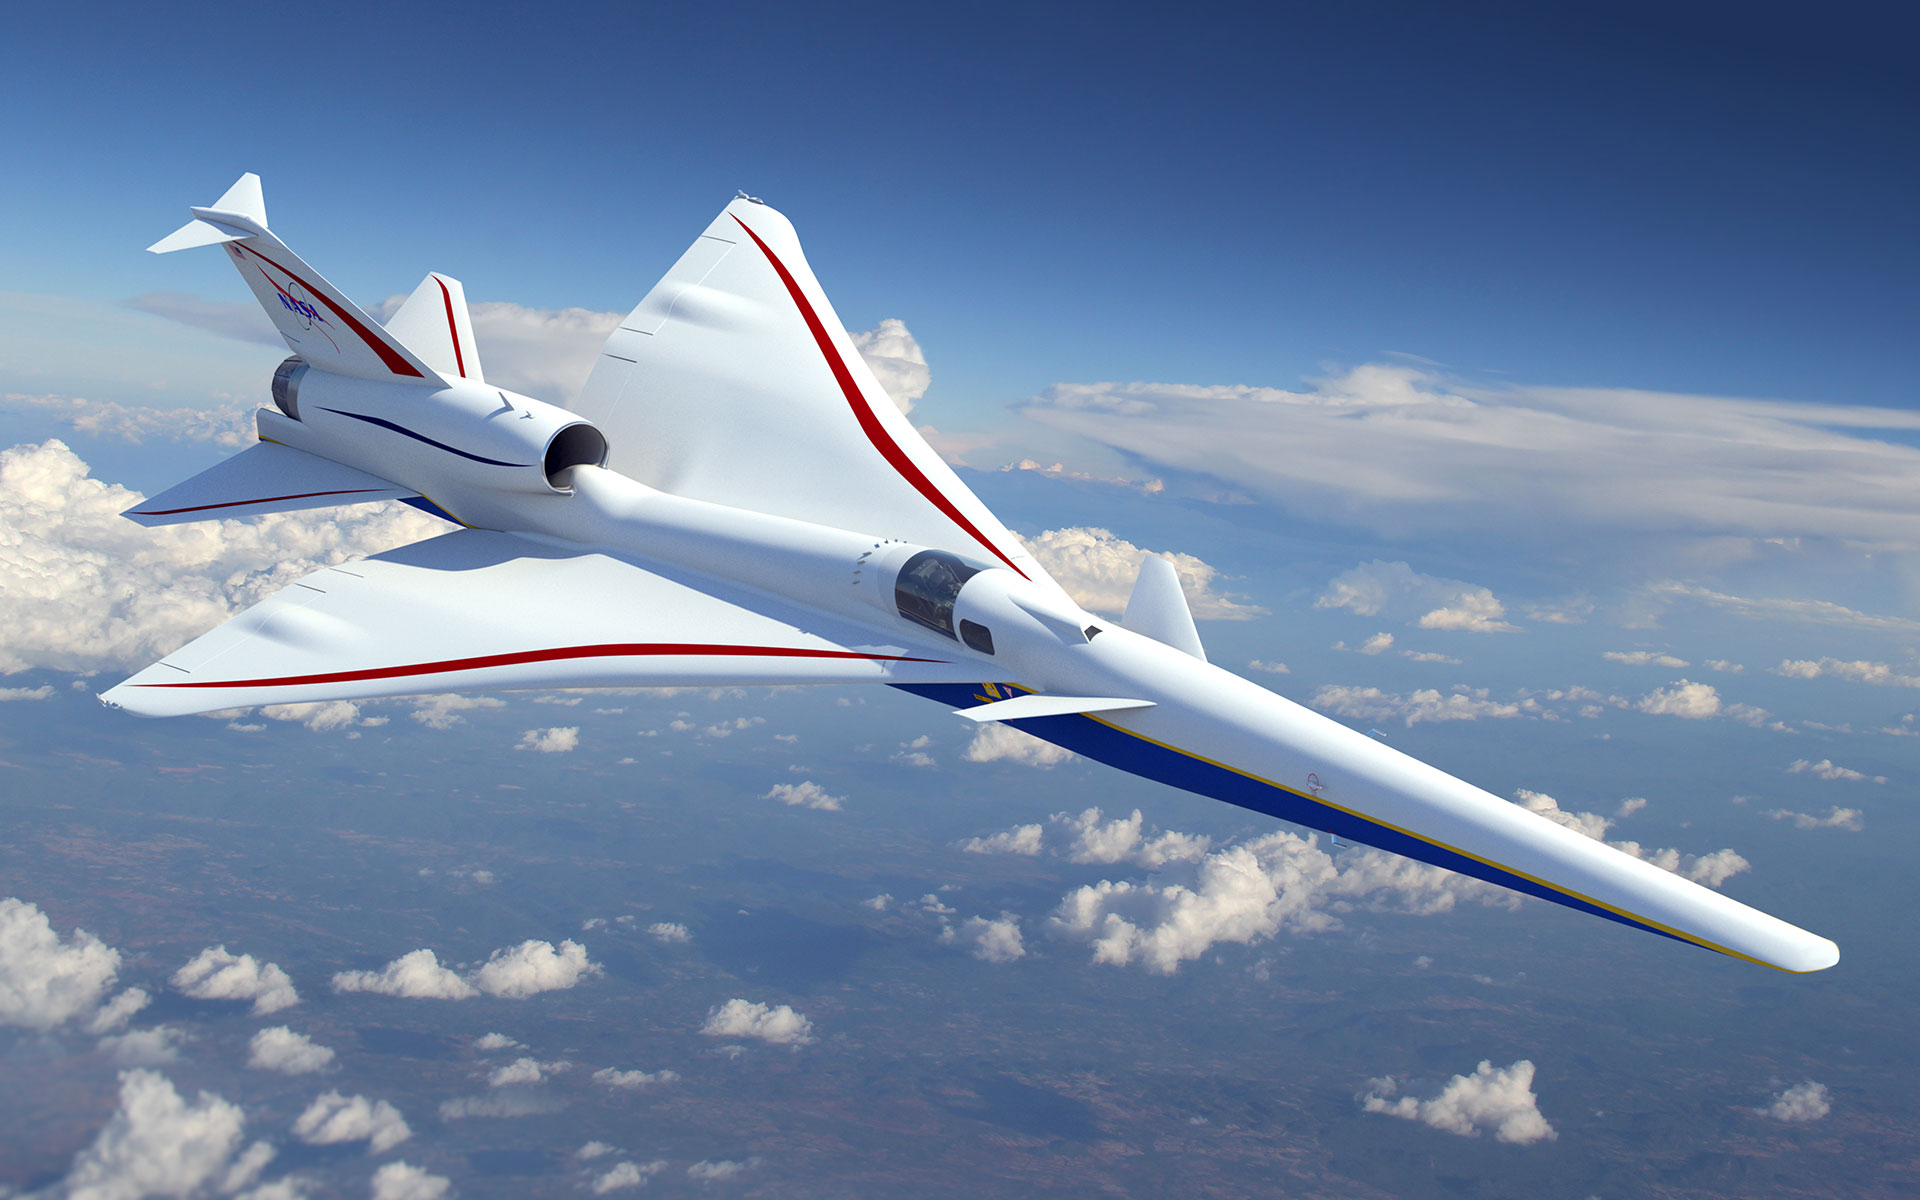
\includegraphics[height=3cm]{../figs/motivation/x59.jpg}};
    \node[anchor=north east, xshift=-2.3cm, yshift=-4.6cm]
      at (current page.north east) {\tiny\color{gray} Source: lockheedmartin.com};
    % https://www.lockheedmartin.com/en-us/products/x-59-quiet-supersonic.html
  \end{tikzpicture}

  \begin{tikzpicture}[remember picture,overlay]
    \node[anchor=north east, xshift=-0.2cm, yshift=-5.2cm]
      at (current page.north east) {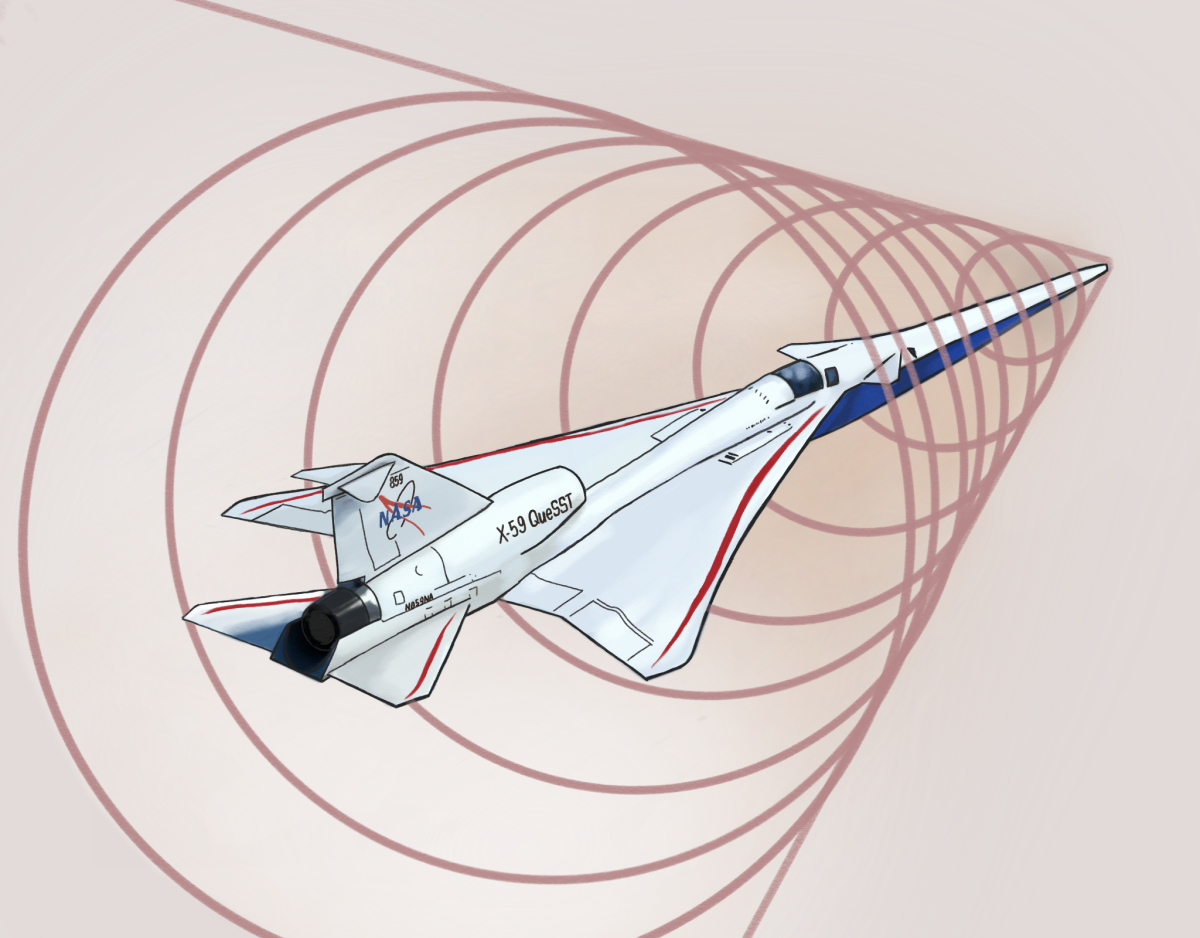
\includegraphics[height=3cm]{../figs/motivation/sonicboomX59Art.png}};
    \node[anchor=north east, xshift=-1.5cm, yshift=-8.3cm]
      at (current page.north east) {\tiny\color{gray} Source: michigandaily.com};
    % https://www.michigandaily.com/opinion/columns/bring-back-the-supersonic-jet-faster/
  \end{tikzpicture}

\end{frame}

%---------------------------------------------------------------%

% TODO: modify last equation to have only dNoise/dpn dpn/dX
%
\stepcounter{sectionframecount}
\begin{frame}[t]{Solution Approach: Broad Picture}
  \begin{minipage}[t]{0.55\linewidth}
    \vspace{-20pt} % This forces the minipage to start at the very top
    Multidisciplinary design optimization\footnotemark:
    \begin{itemize}
      \item Parametric geometry generator.
      \item CFD solver.
      \begin{itemize}
        \item Euler/Navier-Stokes in 3D.
        \item Uniform atmosphere.
      \end{itemize}
      \tikz [remember picture,baseline] \node (start) {};
      \item \textit{Sonic boom propagation tool}
      \begin{itemize}
        \item 2D problem.
        \item Weakly non-linear.
        \item Species relaxation.
        \item Non-uniform atmosphere. \tikz [remember picture,baseline] \node (end) {};
      \end{itemize}
      \vspace{3pt}
      \item Numerical optimizer.
    \end{itemize}
  \end{minipage}

  \begin{minipage}[t]{1\linewidth}
    \vspace{5pt}
    All together:
    $\dfrac{d(\text{Noise})}{dX} = \dfrac{\partial (\text{Noise})}{\partial p_{gs}} \dfrac{\partial p_{gs}}{\partial p_{ns}} \dfrac{d p_{ns}}{d Q} \dfrac{dQ}{dT} \dfrac{dT}{dX}$.
  \end{minipage}

  % Use a TikZ node with 'fit' to enclose the marked area.
  \begin{tikzpicture}[remember picture,overlay]
    \node[draw=red, dashed, thick, inner xsep=8pt, inner ysep=2pt,
          fit=(start) (end), xshift=-2mm, yshift=-0.4mm] {};
  \end{tikzpicture}

  \begin{tikzpicture}[remember picture,overlay]
    \node[anchor=north east, xshift=-0.2cm, yshift=-1.5cm]
      at (current page.north east) {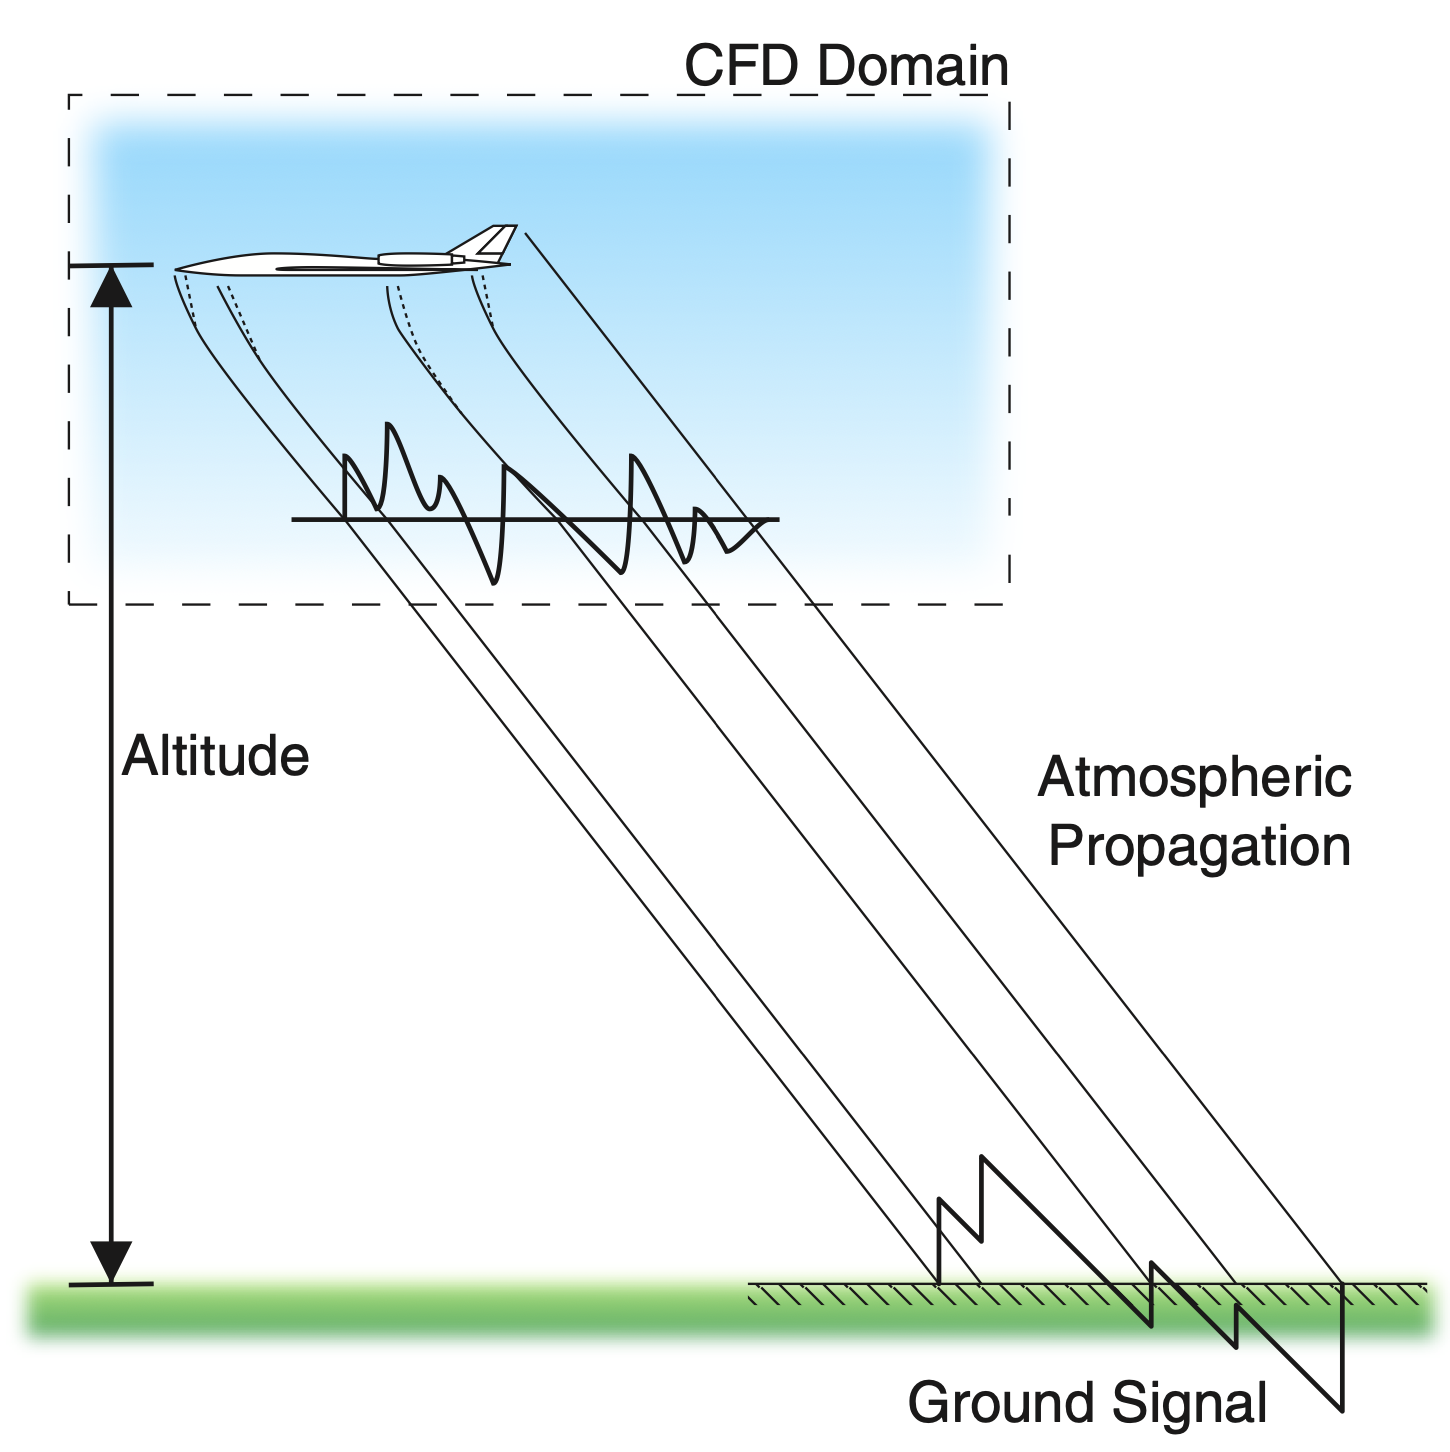
\includegraphics[height=5.5cm]{../figs/motivation/CFDandProp.png}};
    \node[anchor=north east, xshift=-4.4cm, yshift=-6.8cm]
      at (current page.north east) {\tiny\color{gray} Source: [1]};
  \end{tikzpicture}

  \vspace{-8pt}\footnotetext{D. L. Rodriguez et. al. 2025}
\end{frame}

%---------------------------------------------------------------%

\stepcounter{sectionframecount}
\begin{frame}[t]{Propagation Problem: Motivation for Mesh Adaptation}

\vspace{-10pt}
\begin{minipage}[t]{1\linewidth}
  Results for standard time-marching methods\footnotemark:
\end{minipage}

\begin{tikzpicture}[remember picture,overlay]
  \node[anchor=north east, xshift=-8.5cm, yshift=-2.8cm]
    at (current page.north east) {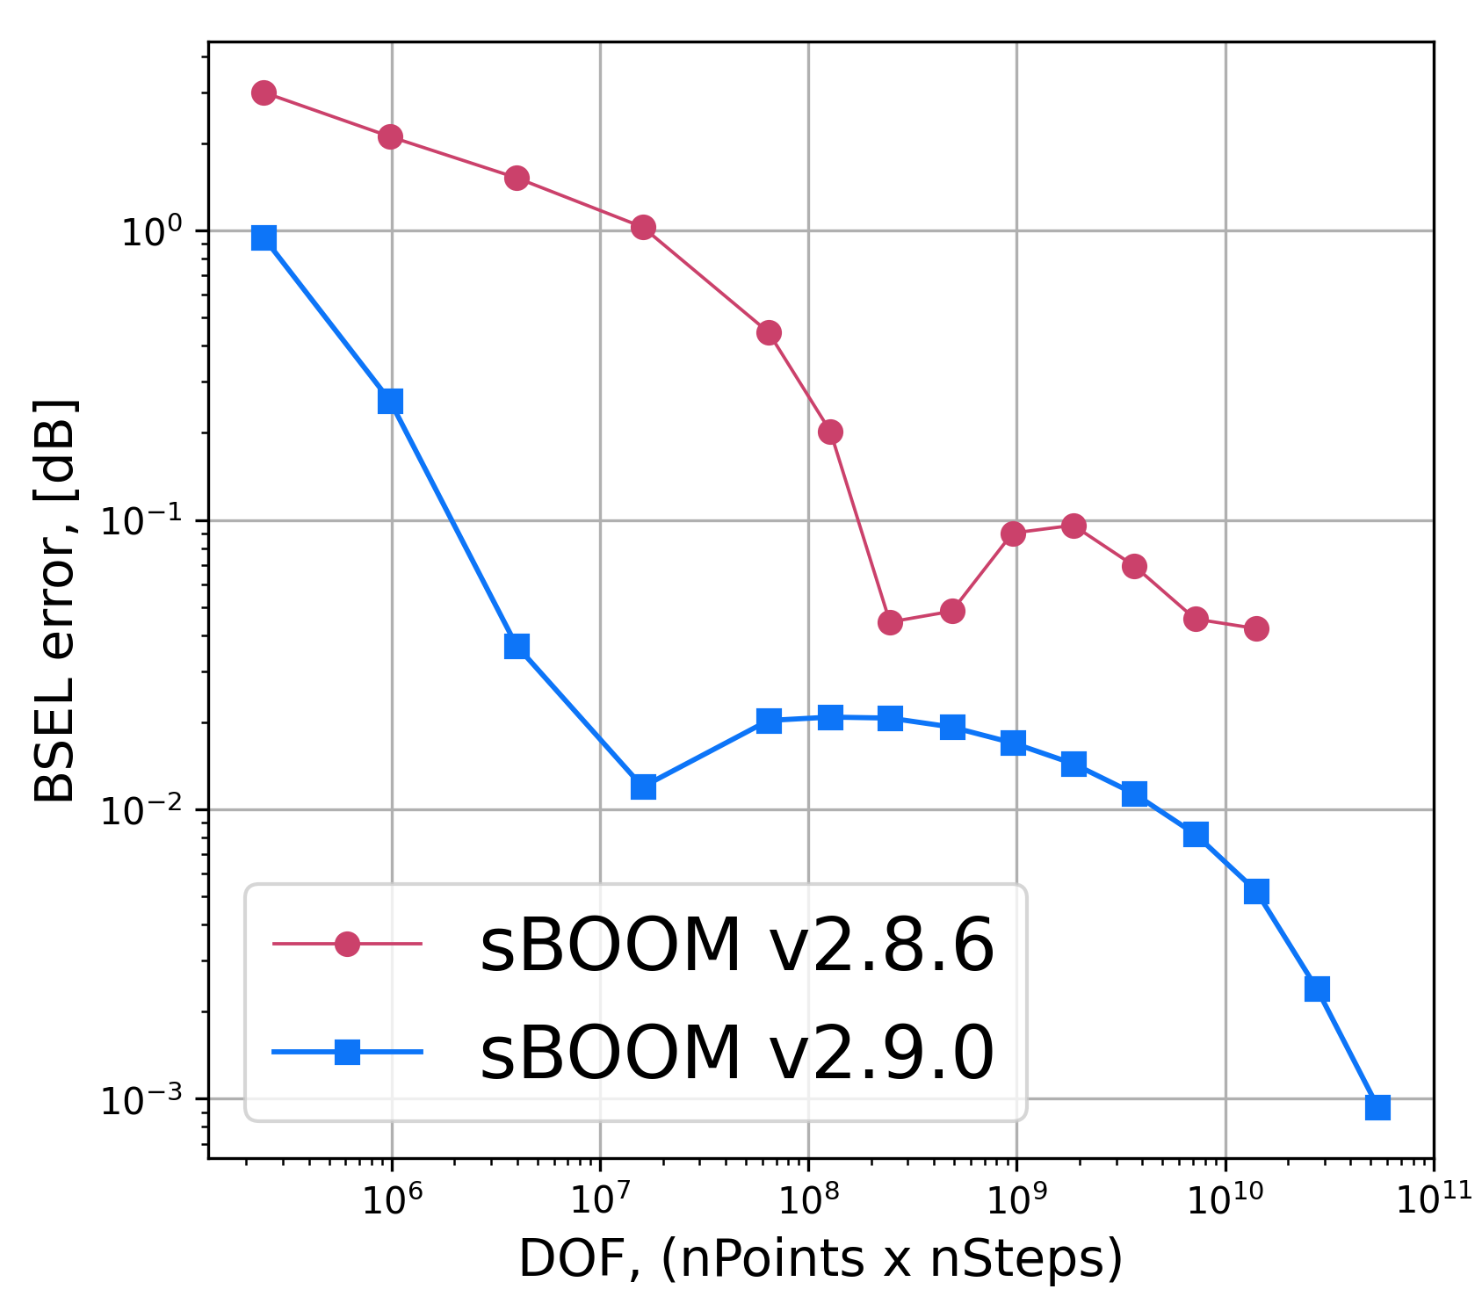
\includegraphics[height=3.5cm]{../figs/motivation/BSELConvergencesBOOM.png}};
  \node[anchor=north east, xshift=-11cm, yshift=-6.4cm]
    at (current page.north east) {\tiny\color{gray} Source: [2]};
\end{tikzpicture}

\begin{tikzpicture}[remember picture,overlay]
  \node[anchor=north east, xshift=-1.5cm, yshift=-2.8cm]
    at (current page.north east) {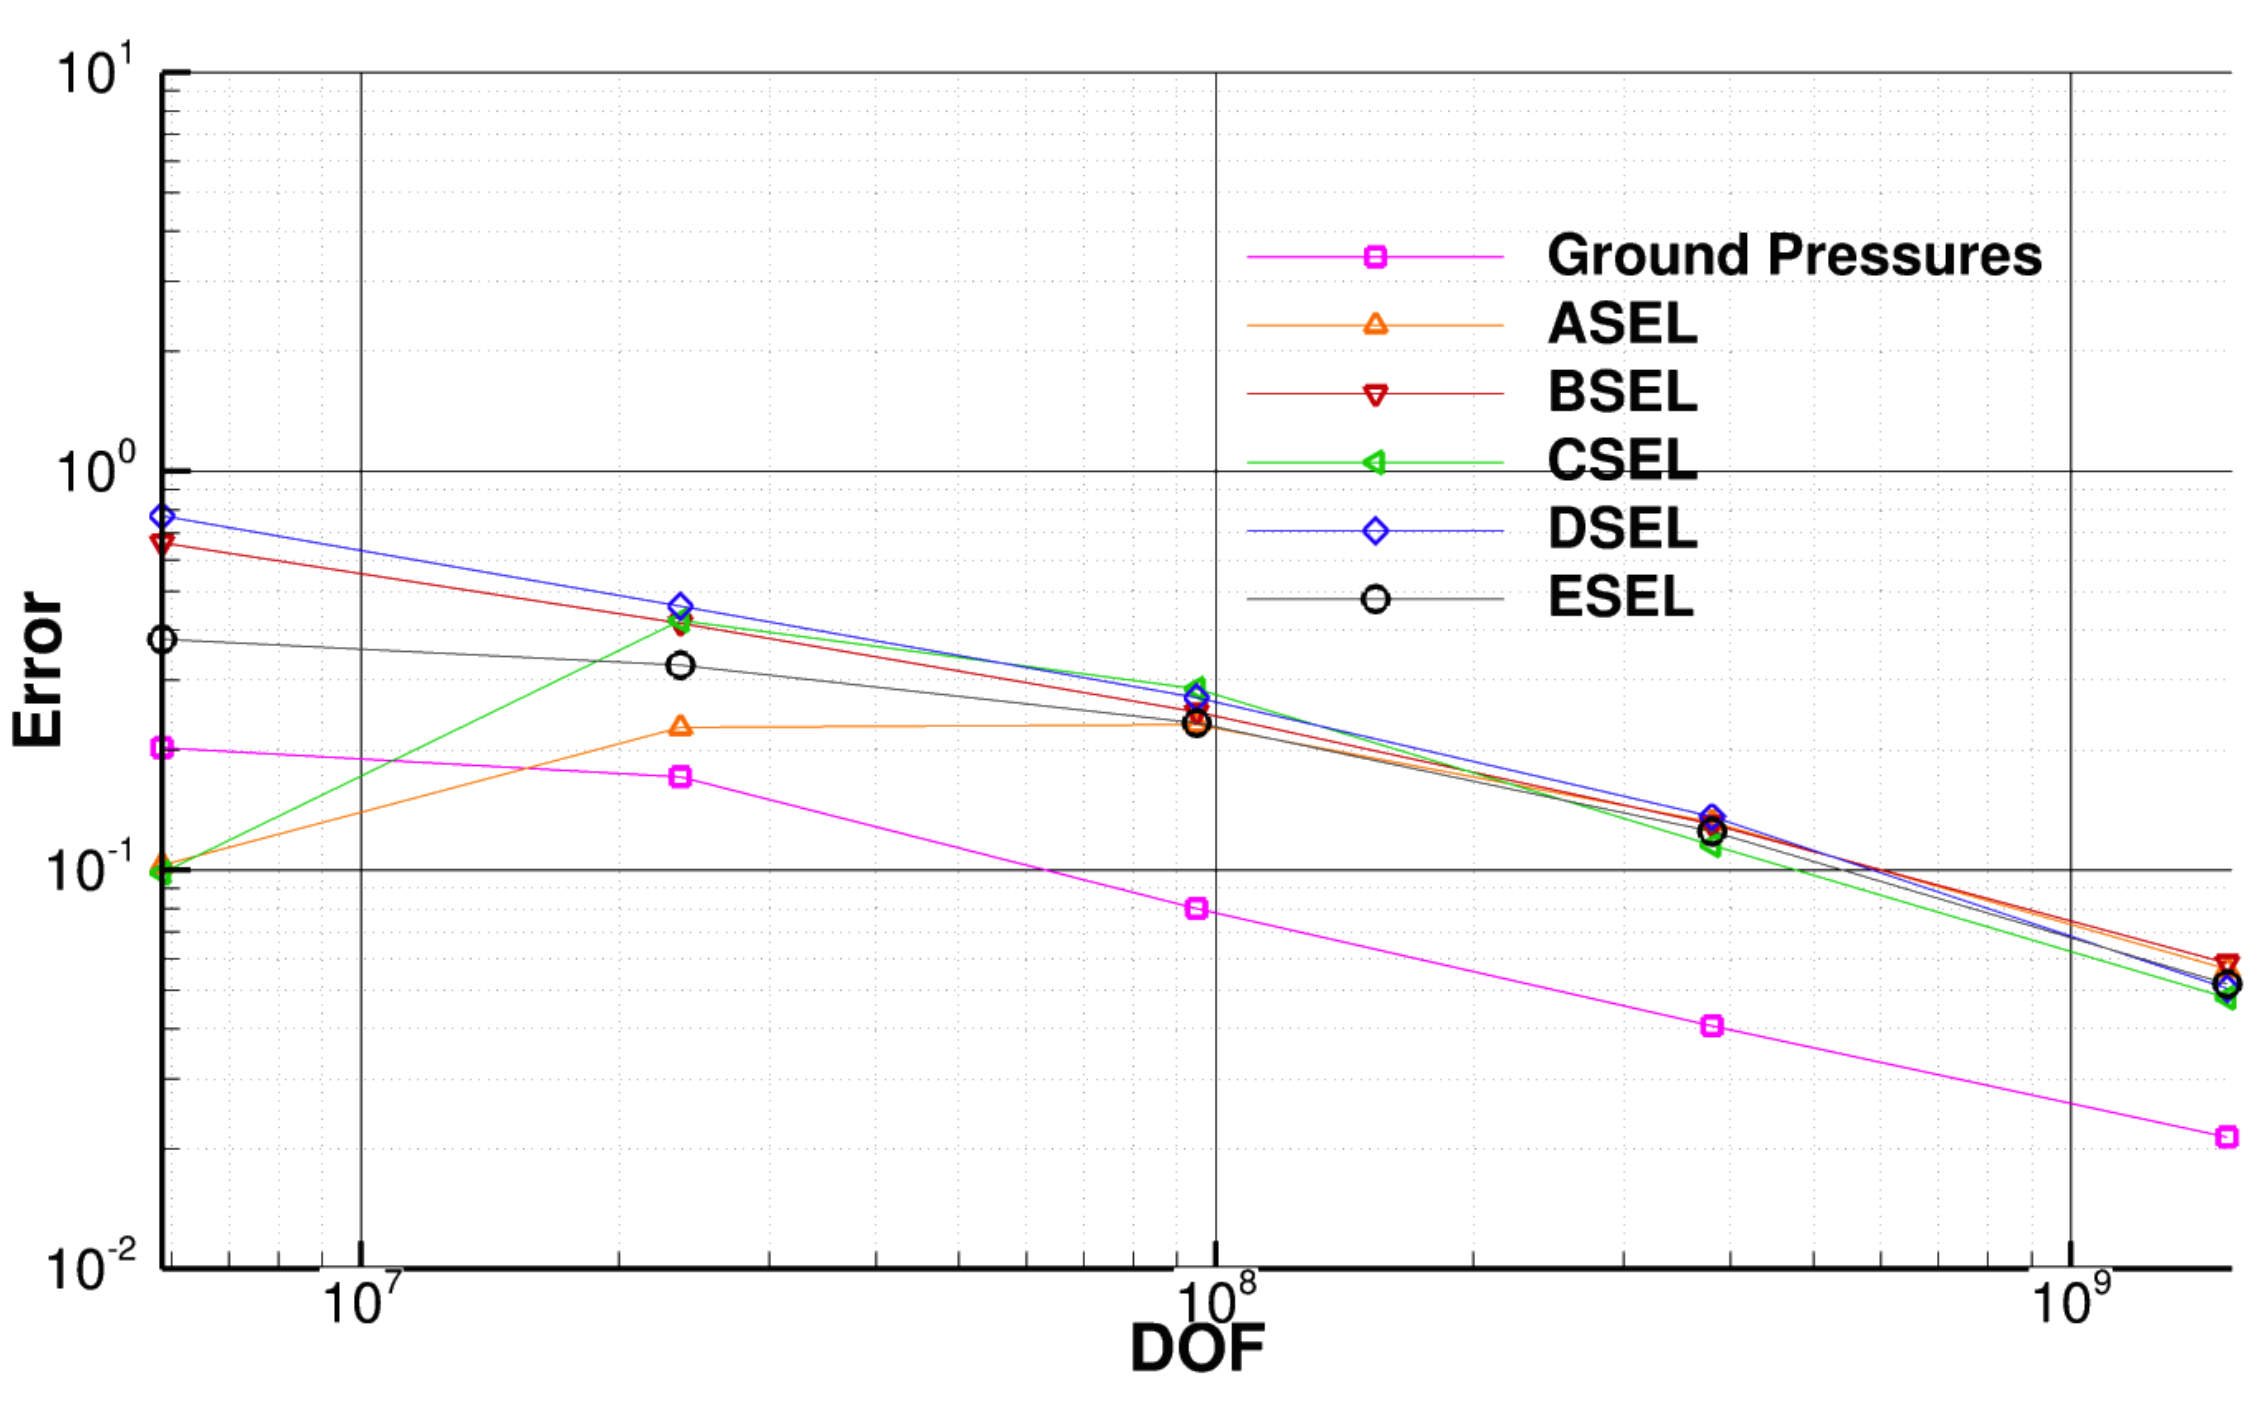
\includegraphics[height=3.5cm]{../figs/motivation/sensitivityNormErrorsBOOM.png}};
  \node[anchor=north east, xshift=-5.5cm, yshift=-6.4cm]
    at (current page.north east) {\tiny\color{gray} Source: [2]};
\end{tikzpicture}

\vspace{3.5cm}
\begin{minipage}[t]{1\linewidth}
  \textbf{Our goal:}
  Reduce the significant computational cost involved. Enable efficient, automated high accuracy predictions of boom propagation and design sensitivities through adaptive control of numerical error.
\end{minipage}

\vspace{-8pt}\footnotetext{S. K. Rallabhandi et. al. 2023}

\end{frame}

%---------------------------------------------------------------%

% TODO: include titles in the figures

\stepcounter{sectionframecount}
\begin{frame}[t]{Propagation Problem: Space-time Adaptive Method}

\begin{tikzpicture}[remember picture,overlay]
  \node[anchor=north east, xshift=-0.5cm, yshift=-1.5cm]
    at (current page.north east) {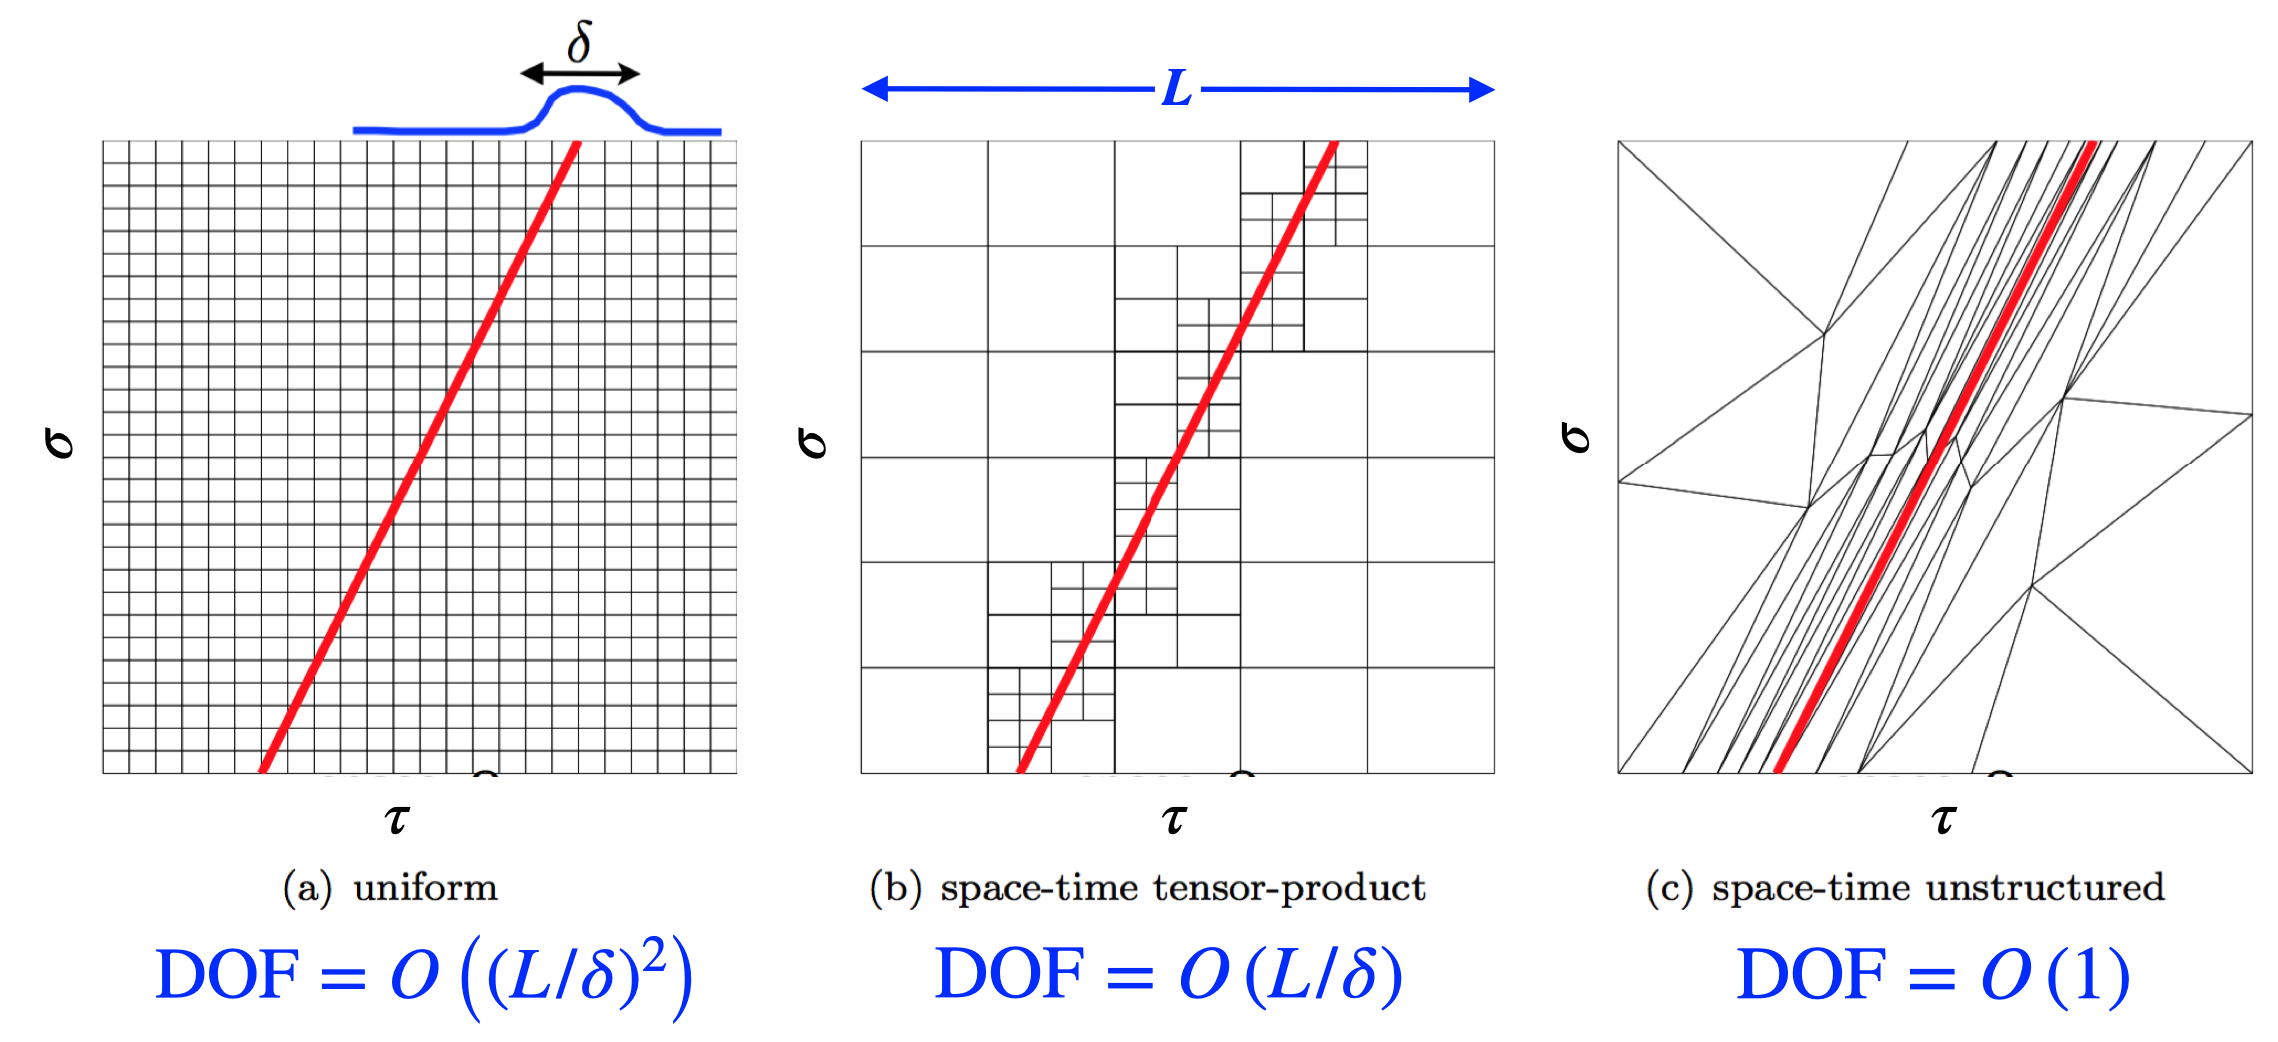
\includegraphics[height=5.5cm]{../figs/motivation/spaceTimeAdaptiveMethod.png}};
\end{tikzpicture}

\begin{minipage}[t]{1\linewidth}
  \vspace{4.8cm}
  But, space-time unstructured requires coupled solve over entire space-time domain.
\end{minipage}

\end{frame}

%---------------------------------------------------------------%

% TODO: hold off this one a bit, for after boom modeling and before shock capturing

\stepcounter{sectionframecount}
\begin{frame}[t]{Propagation Problem: Methodology Overview}
  \vspace{20pt}
  \begin{minipage}[t]{1\linewidth}
    \begin{enumerate}
      \item Boom Propagation Modeling.
      \vspace{10pt}
      \item Shock Capturing.
      \vspace{10pt}
      \item Ground Signal Filtering.
      \vspace{10pt}
      \item FEM Discretization and Output Error Estimation.
      \vspace{10pt}
      \item Output-based Mesh Adaptation.
    \end{enumerate}

  \end{minipage}
\end{frame}

%=============================================================================%
%=============================================================================%
%=============================================================================%
% Section: Boom propagation modeling

\begin{frame}[plain]
  \vfill
  \centering
  {\usebeamerfont{title}\usebeamercolor[fg]{title}Boom Propagation Modeling}
  \vfill
\end{frame}


\section{Boom Propagation Modeling}

\setsectionframes{3}

%---------------------------------------------------------------%

\stepcounter{sectionframecount}
\begin{frame}[t]{Coordinate System}
  \vspace{-8pt}
  Airplane at cruise altitude and cruise Mach number ($M_a$):

  \begin{tikzpicture}[remember picture,overlay]
    \node[anchor=north east, xshift=-1.1cm, yshift=-2.1cm]
    at (current page.north east) {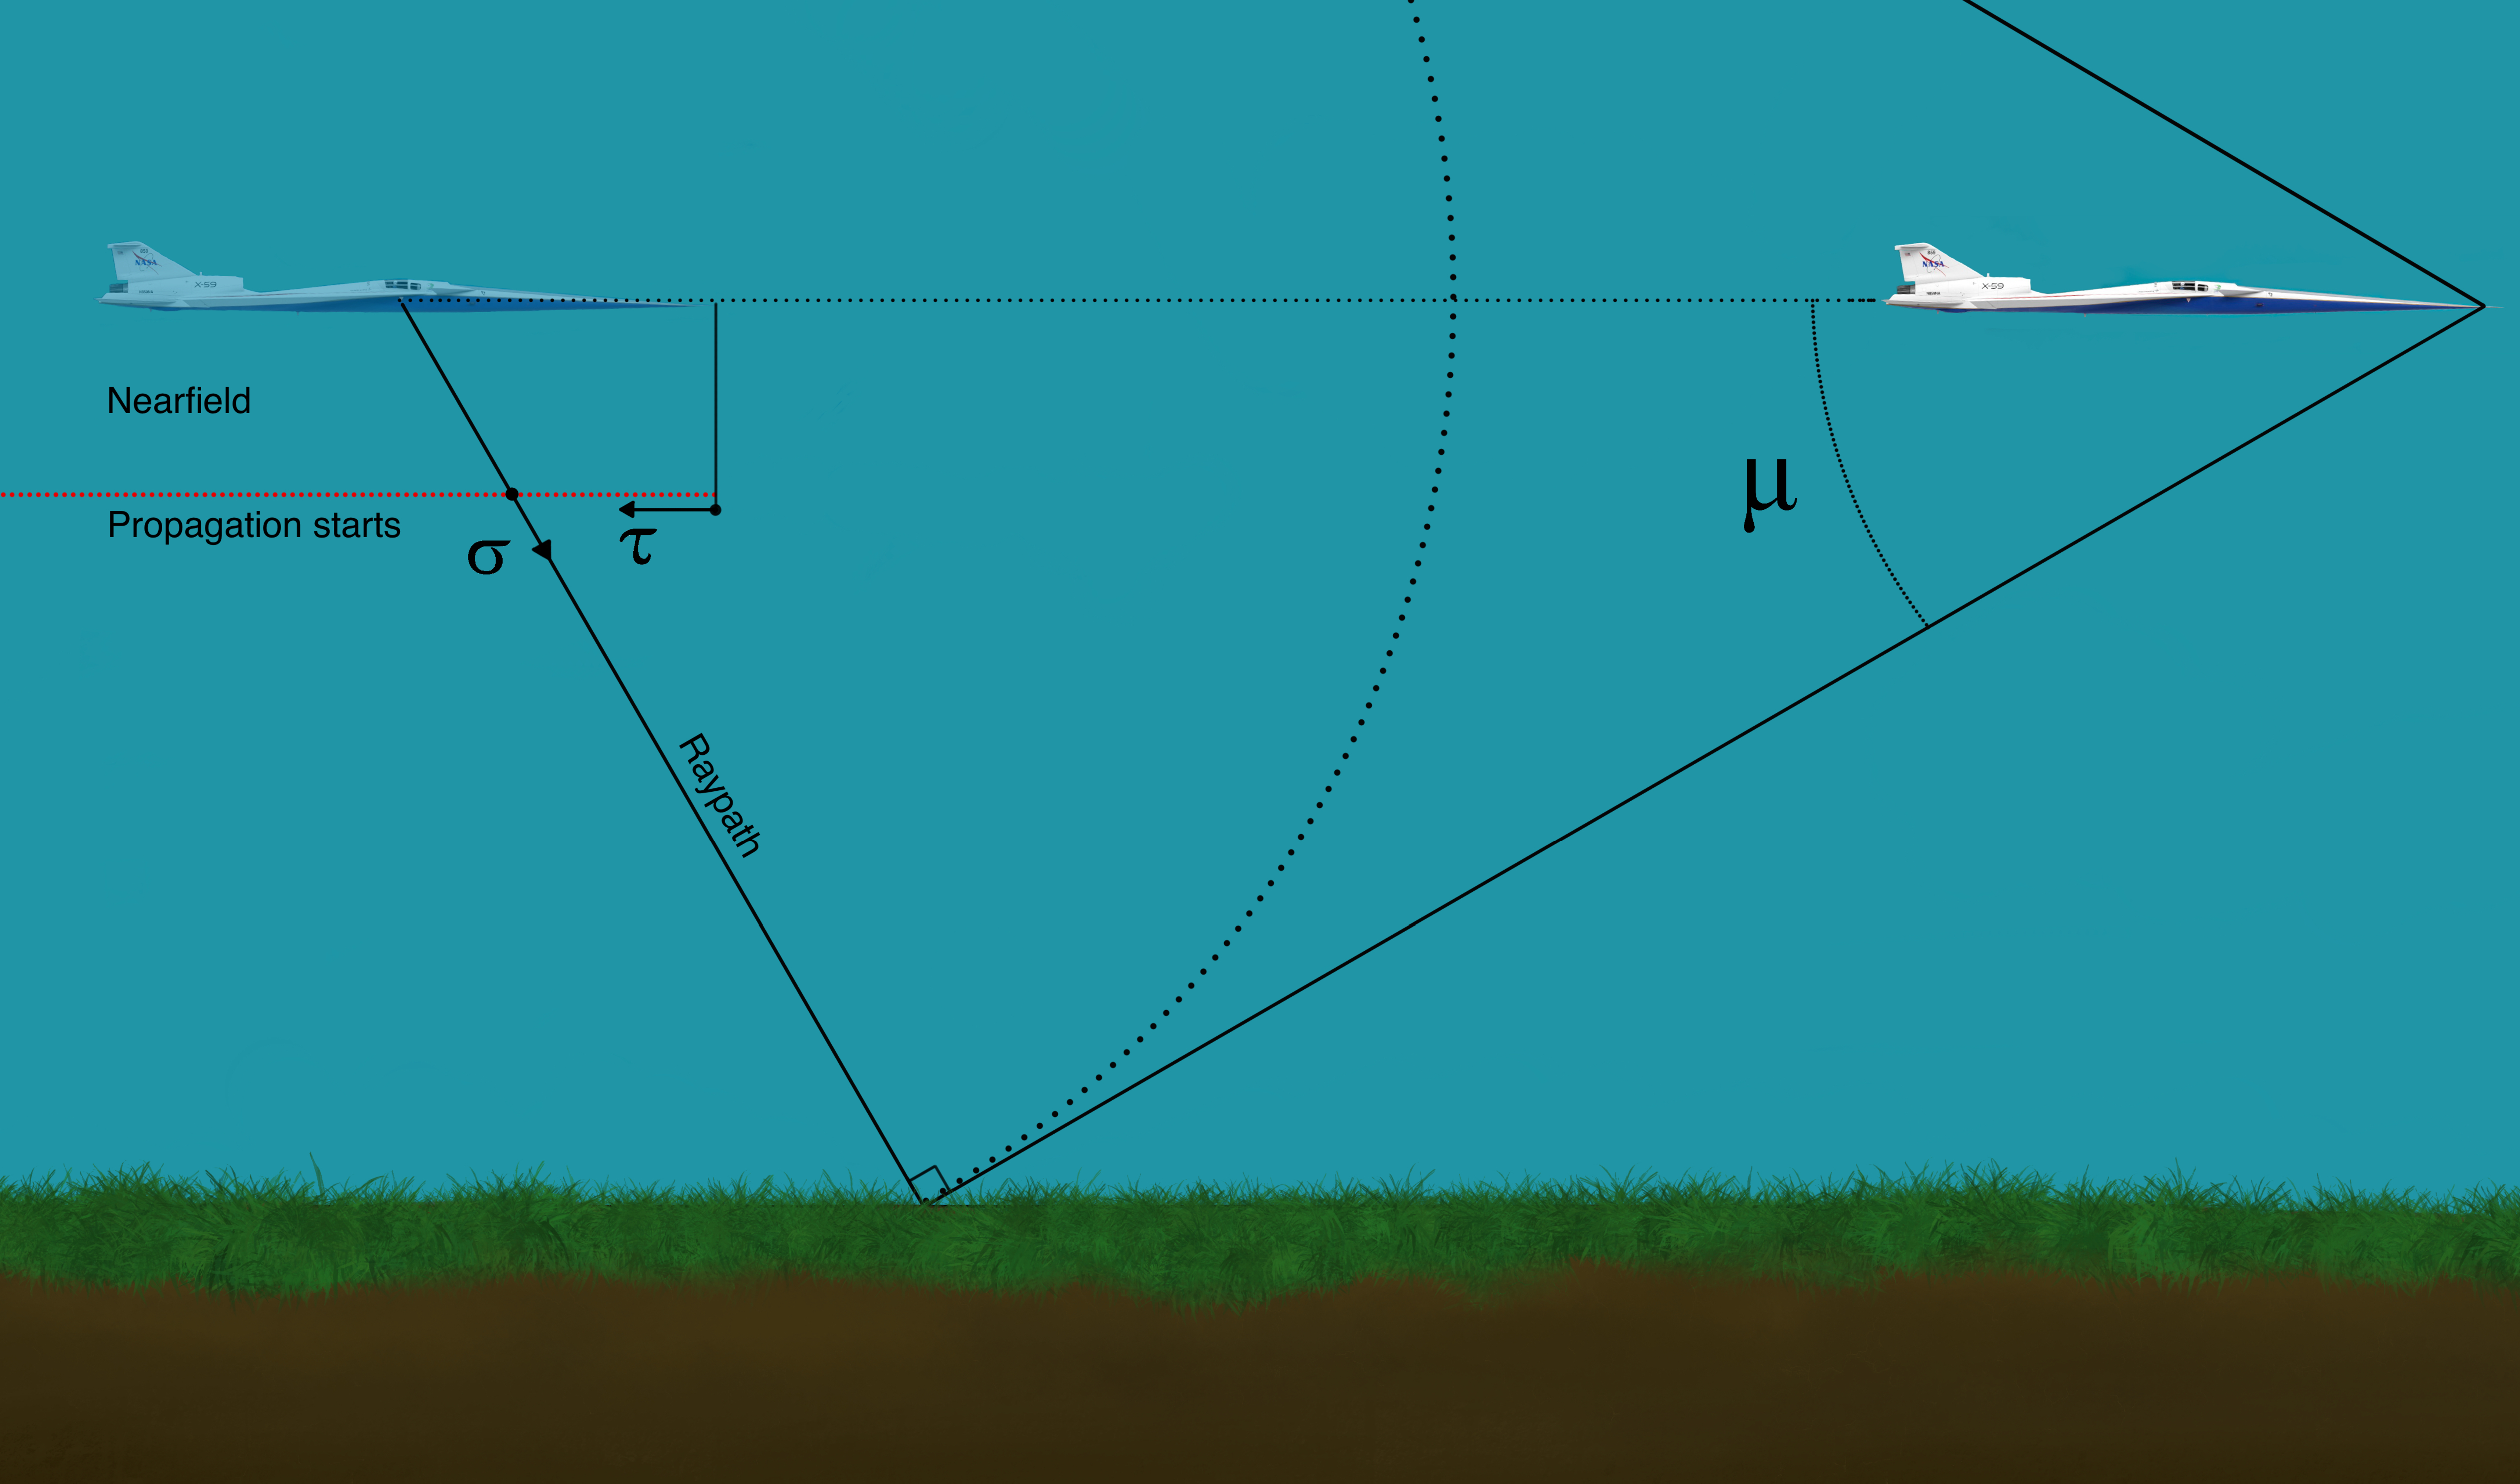
\includegraphics[height=6cm]{../figs/boom_modeling/Coordinate_System_.pdf}};
  \end{tikzpicture}

  \vspace{6cm}
  Mach cone angle: $\mu = \sin^{-1}(1/M_a)$.

\end{frame}

%---------------------------------------------------------------%

% TODO: mention parabolic equation, sigma is time-like direction
% TODO: time-marching in sigma direction as the typical way of solving it

\stepcounter{sectionframecount}
\begin{frame}[t]{Augmented Burgers System}
  To model sonic boom propagation we use the augmented Burgers system of equations:

  \begin{equation}
    \dfrac{\partial P}{\partial \sigma}
    -\dfrac{1}{2}\dfrac{\partial \ln(\rho_0c_0/A_{n0})}{\partial \sigma}P
    -\dfrac{1}{2}\dfrac{\partial P^2}{\partial \tau}
    -\dfrac{1}{\Gamma}\dfrac{\partial ^2 P}{\partial \tau^2}
    -\dfrac{\partial }{\partial \tau}\left(\sum_{\nu} C_\nu \dfrac{\partial\tilde{P}_\nu}{\partial \tau}\right)
    =0,
  \end{equation}

  \begin{equation}
    -\dfrac{\partial \tilde{P}_\nu}{\partial \tau} + \dfrac{P - \tilde{P}_\nu}{\theta_\nu} = 0,~~~~\nu = \{\text{O}_2,\text{N}_2\},
  \end{equation}
  which includes:
  \begin{itemize}
    \item Thermoviscous diffusion.
    \item Atmospheric absorption by relaxation species (O$_2$ and N$_2$).
    \item Ray tube area variation.
  \end{itemize}

\end{frame}

%---------------------------------------------------------------%

\stepcounter{sectionframecount}
\begin{frame}[t]{Atmosphere Model: Standard}

Atmosphere model refers to how the atmospheric properties depend on altitude.

\textbf{Standard model:} First two layers:

\begin{tikzpicture}[remember picture,overlay]
  \node[anchor=north east, xshift=-5.5cm, yshift=-3.5cm]
  at (current page.north east) {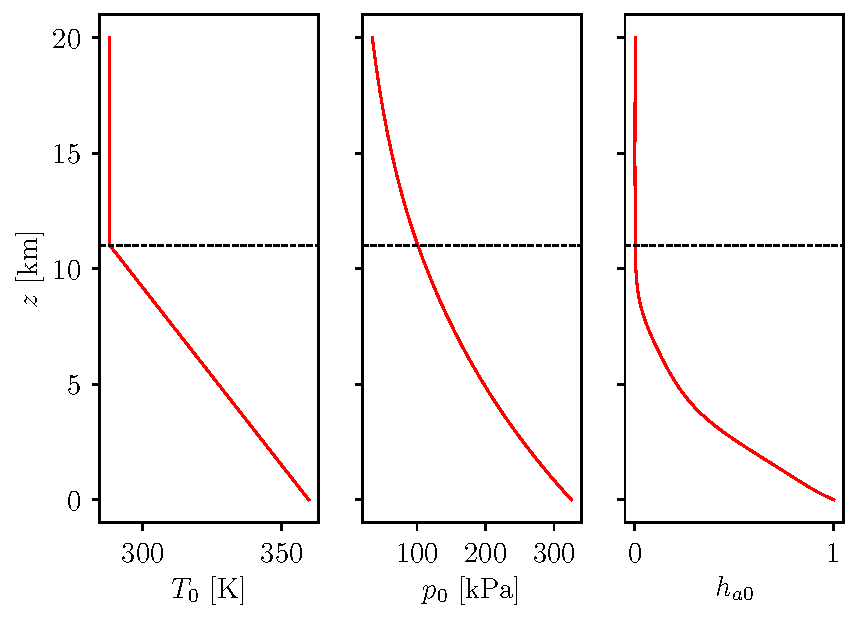
\includegraphics[height=5.0cm]{../figs/boom_modeling/atmosphereStandard.pdf}};
\end{tikzpicture}

\begin{tikzpicture}[remember picture,overlay]
  % Place the minipage 1cm from the left and 1cm down from the top
  \node[anchor=north east, xshift=-0.2cm, yshift=-2.8cm] at (current page.north east) {%
    \begin{minipage}{0.4\textwidth}
      \textbf{Additionally, models for:}
      \par\medskip
      \begin{itemize}
        \item Density and speed of sound: $\rho_0$, $c_0$,
        \item Gol'berg number: $\Gamma$,
        \item Relaxation coefficients: $C_\nu, \theta_\nu$,
        \item Ray tube area: $A_{n0}$,
      \end{itemize}

      as functions of atmospheric properties.
    \end{minipage}
  };
\end{tikzpicture}

\end{frame}

%--------------
% put space-time adaptive approach here

%=============================================================================%
%=============================================================================%
%=============================================================================%
% Section: Shock capturing

\begin{frame}[plain]
  \vfill
  \centering
  {\usebeamerfont{title}\usebeamercolor[fg]{title}Shock Capturing}
  \vfill
\end{frame}


\section{Discretization and Shock Capturing}

% TODO: refactor section. put burgers + av at the top
% then say how e_av is computed using the sensor value
% and then say how the sensor is defined

\setsectionframes{6}

%---------------------------------------------------------------%

\stepcounter{sectionframecount}
\begin{frame}[t]{The Need for Artificial Viscosity}
\textbf{Challenge:} Discontinuities (shocks) in the solutions, leading to unstable
numerical solves and lack of convergence.

\vspace{20pt}
\textbf{Goal:} Smoothen discontinuities to improve stability, while not modifying
the already smooth areas.

\vspace{20pt}
\textbf{Solution Approach:} Employ a shock sensor, $s$, to keep track of discontinuities, and use that information to add localized artificial viscosity.

\vspace{8pt}
\begin{itemize}
  \item Shock sensor design requirements:
  \begin{itemize}
    \item $s \approx 1$ in shock areas.
    \item $s \approx 0$ away from shocks.
    \item Order $\mathcal{O}(h^p)$.
    \item $s$ smooth.
  \end{itemize}
\end{itemize}

\end{frame}

%---------------------------------------------------------------%

\stepcounter{sectionframecount}
\begin{frame}[t]{PDE-based Shock Sensor\footnotemark}

The shock sensor becomes a state itself, $s$, with its own equation:

\begin{equation}
  \underbrace{s - C_1s_{\text{grad}}}_{\text{source term}} + \underbrace{\dfrac{C_2}{p^2}\nabla \cdot \left(H^2_{00}\dfrac{\partial s}{\partial \tau} + H^2_{01}\dfrac{\partial s}{\partial \sigma},H^2_{10}\dfrac{\partial s}{\partial \tau}+H^2_{11}\dfrac{\partial s}{\partial \sigma}\right)}_{\text{diffusion term}} = 0.
	\label{e:sensor_source}
\end{equation}

\begin{itemize}
  \item $s_{\text{grad}}$: Shock indicator based on pressure solution gradient.
  \item $p$: polynomial solution order.
  \item $H$: element size field.
  \item Diffusion term: to have a smooth sensor solution.
\end{itemize}

\footnotetext{G. E. Barter and D. L. Darmofal 2007}
\end{frame}

%---------------------------------------------------------------%

% TODO: keep eq 4, removing the max thing
% TODO: remove explicit formula (save as back-up)

\stepcounter{sectionframecount}
\begin{frame}[t]{Shock Indicator $s_{\text{grad}}$}

  Starting point:
  \begin{equation}
    \xi := \dfrac{H_{\tau\tau}}{p} \left|\dfrac{\partial P}{\partial \tau}\right|,~~~~ \xi_1 \simeq \max_{x\in\Omega} \xi(x),~~~\hat{\xi} = \dfrac{\xi}{\xi_1},
  \end{equation}
  then:
  \begin{equation}
    s_\text{grad} := s_\text{grad}(\hat{\xi}) = \dfrac{\hat{\xi} [\tanh(p^2\hat{\xi})]^{p-1}}{1+\exp\left[-k \left(\hat{\xi} - \alpha(p)\right)\right]},
    \label{e:s_grad}
  \end{equation}
  where $k,\alpha(p) \in \mathbb{R}$.
\end{frame}

%---------------------------------------------------------------%

% TODO: dash line for linear case
% TODO: combine with previous one

\stepcounter{sectionframecount}
\begin{frame}[t]{Shock Indicator $s_{\text{grad}}$}
  \vspace{-10pt}
  \begin{equation}
    \small
    s_\text{grad} := s_\text{grad}(\hat{\xi}) = \dfrac{\hat{\xi} [\tanh(p^2\hat{\xi})]^{p-1}}{1+\exp\left[-k \left(\hat{\xi} - \alpha(p)\right)\right]},
    \label{e:s_grad}
  \end{equation}

  \begin{tikzpicture}[remember picture,overlay]
    \node[anchor=north east, xshift=-2.5cm, yshift=-3.2cm]
    at (current page.north east) {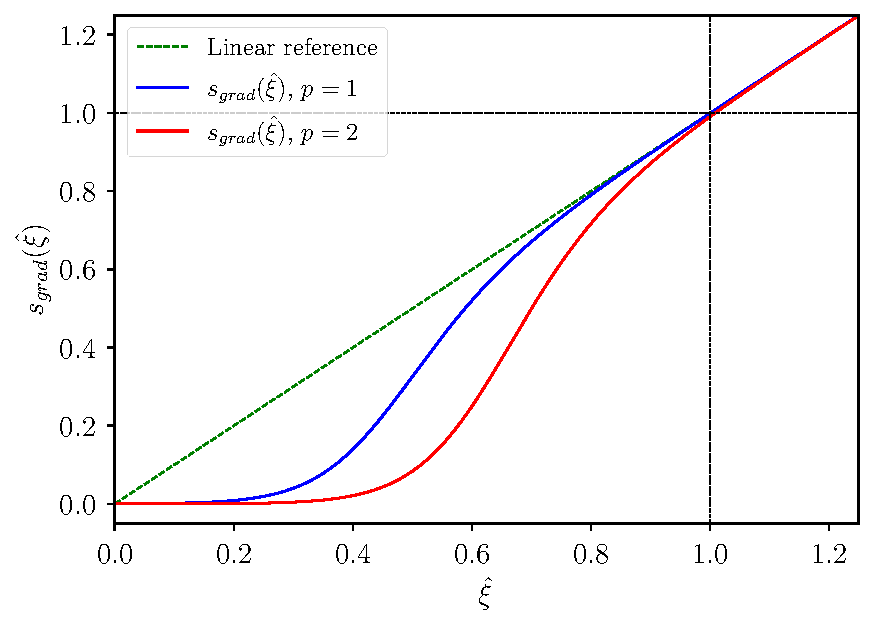
\includegraphics[height=5.7cm]{../figs/shock_capturing/s_grad.pdf}};
  \end{tikzpicture}
  \end{frame}

%---------------------------------------------------------------%

% TODO: flip order of equations
% TODO: put this slide above and combine with sensor equation slide

\stepcounter{sectionframecount}
\begin{frame}[t]{Addition of Artificial Viscosity to the Burgers Equation}
Compute artificial viscosity coefficient $\epsilon_{\text{AV}}$:

\begin{equation}
  \epsilon_{\text{AV}} := \dfrac{1}{2}\dfrac{H_{00}}{p}|P|s.
\end{equation}

Add extra diffusion term in Burgers equation:

\begin{equation}
  \small
  \dfrac{\partial P}{\partial \sigma}
  -\dfrac{1}{2}\dfrac{\partial \ln(\rho_0c_0/A_{n0})}{\partial \sigma}P
  -\dfrac{1}{2}\dfrac{\partial P^2}{\partial \tau}
  -\dfrac{1}{\Gamma}\dfrac{\partial ^2 P}{\partial \tau^2}
  -\dfrac{\partial }{\partial \tau}\left(\sum_{\nu} C_\nu \dfrac{\partial\tilde{P}_\nu}{\partial \tau}\right)
  \underbrace{- \dfrac{\partial}{\partial \tau} \left(\epsilon_{\text{AV}}\dfrac{\partial P}{\partial \tau}\right)}_{\text{extra term}}
  =0.
\end{equation}

\end{frame}

%---------------------------------------------------------------%

% TODO: repeat this slide putting the different plots one at a time

\stepcounter{sectionframecount}
\begin{frame}[t]{Test With Smooth Problem}
\vspace{-10pt}
Smooth problem with available exact solution:

\begin{itemize}
  \item Solve without artificial viscosity.
  \item Solve with artificial viscosity and see how it affects convergence.
\end{itemize}

\begin{tikzpicture}[remember picture,overlay]
  % Place the minipage 1cm from the left and 1cm down from the top
  \node[anchor=north east, xshift=-4.3cm, yshift=-3.7cm] at (current page.north east) {%
    \begin{minipage}{0.5\textwidth}
    Solution L2 error

    \end{minipage}
  };
\end{tikzpicture}

\begin{tikzpicture}[remember picture,overlay]
  % Place the minipage 1cm from the left and 1cm down from the top
  \node[anchor=north east, xshift=2cm, yshift=-3.7cm] at (current page.north east) {%
    \begin{minipage}{0.5\textwidth}
    Output error

    \end{minipage}
  };
\end{tikzpicture}

\begin{tikzpicture}[remember picture,overlay]
  \node[anchor=north east, xshift=-6cm, yshift=-4.1cm]
  at (current page.north east) {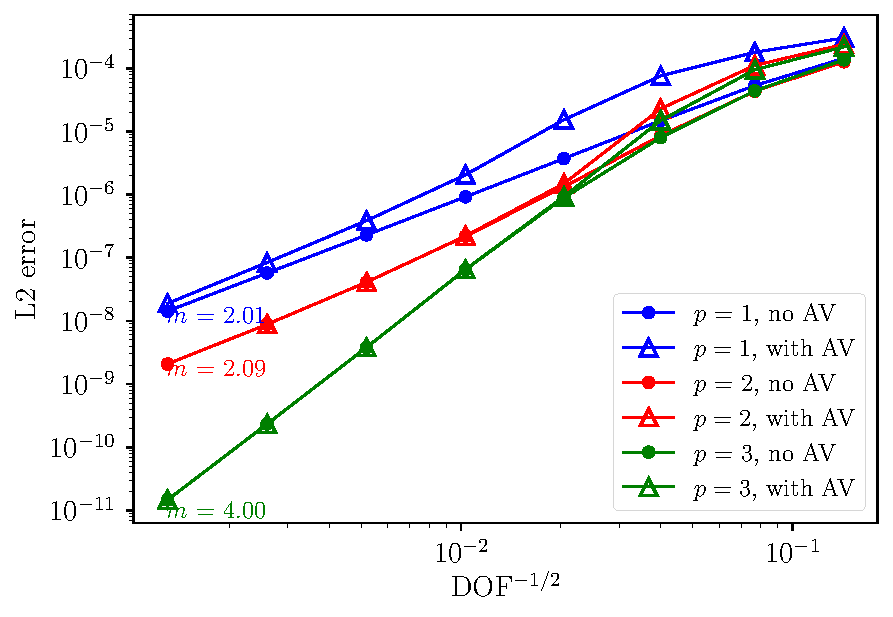
\includegraphics[height=4.5cm]{../figs/shock_capturing/primal_traveling_wave_withAV_L2_UniRef.pdf}};
\end{tikzpicture}

\begin{tikzpicture}[remember picture,overlay]
  \node[anchor=north east, xshift=0cm, yshift=-4.1cm]
  at (current page.north east) {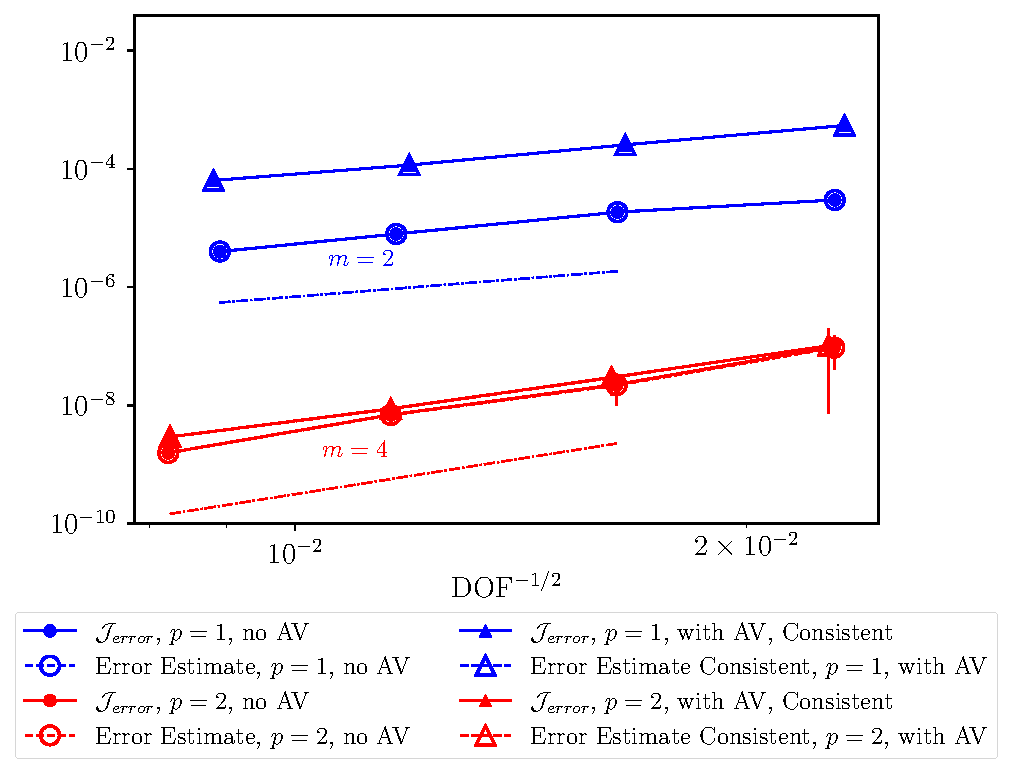
\includegraphics[height=4.5cm]{../figs/shock_capturing/OutputErrorTravelingWave_Consistent_adaptive.pdf}};
\end{tikzpicture}

\end{frame}

%=============================================================================%
%=============================================================================%
%=============================================================================%
% Ground signal filtering

\begin{frame}[plain]
  \vfill
  \centering
  {\usebeamerfont{title}\usebeamercolor[fg]{title}Ground Signal Filtering}
  \vfill
\end{frame}


\section{Ground Signal Filtering}

\setsectionframes{3}

%---------------------------------------------------------------%

\stepcounter{sectionframecount}
\begin{frame}[t]{Relevant Loudness Metrics}
The human ear is less sensitive to low audio frequencies.

\vspace{10pt}
There is a family of weighting filter curves that account for this relative loudness perceived by humans: A/B/C/D/-SEL curves.

\vspace{10pt}
(Ground pressure signal) $p(t)\to \text{ Weighting filter }\to \tilde{p}(t)$ (Filtered signal)

\vspace{10pt}
Sound exposure:

\begin{equation}
  E = \int_{t_0}^{t_{\text{f}}} \tilde{p}(t)~dt.
\end{equation}

\vspace{10pt}
Loudness level in dB:

\begin{equation}
  \text{Loudness} = 10\log_{10}\left(\dfrac{E}{E_0}\right),~~~ E_0 = 400~ (\mu\text{Pa})^2s.
\end{equation}

\end{frame}

%---------------------------------------------------------------%

\stepcounter{sectionframecount}
\begin{frame}[t]{B-SEL Metric}
\vspace{-10pt}
We focus on the B-SEL curve, and the approach can be generalized to any other.

\vspace{10pt}
Transfer function in the complex frequency domain:

\begin{equation}
  H_B(s) =\dfrac{\tilde{P}(s)}{P(s)} = \dfrac{c_B s^3}{(s+2\pi f_1)^2(s+2\pi f_{2B})(s+2\pi f_4)^2},
  \label{e:continuous_transfer}
\end{equation}

\vspace{10pt}
\begin{itemize}
  \item $c_B = 5.99185 \times 10^9$
  \item $f_1 = 20.598997$ Hz
  \item $f_{2B} = 158.48932$ Hz
  \item $f_4 = 12194.217$ Hz
\end{itemize}

\begin{tikzpicture}[remember picture,overlay]
  \node[anchor=north east, xshift=0.5cm, yshift=-4.5cm]
  at (current page.north east) {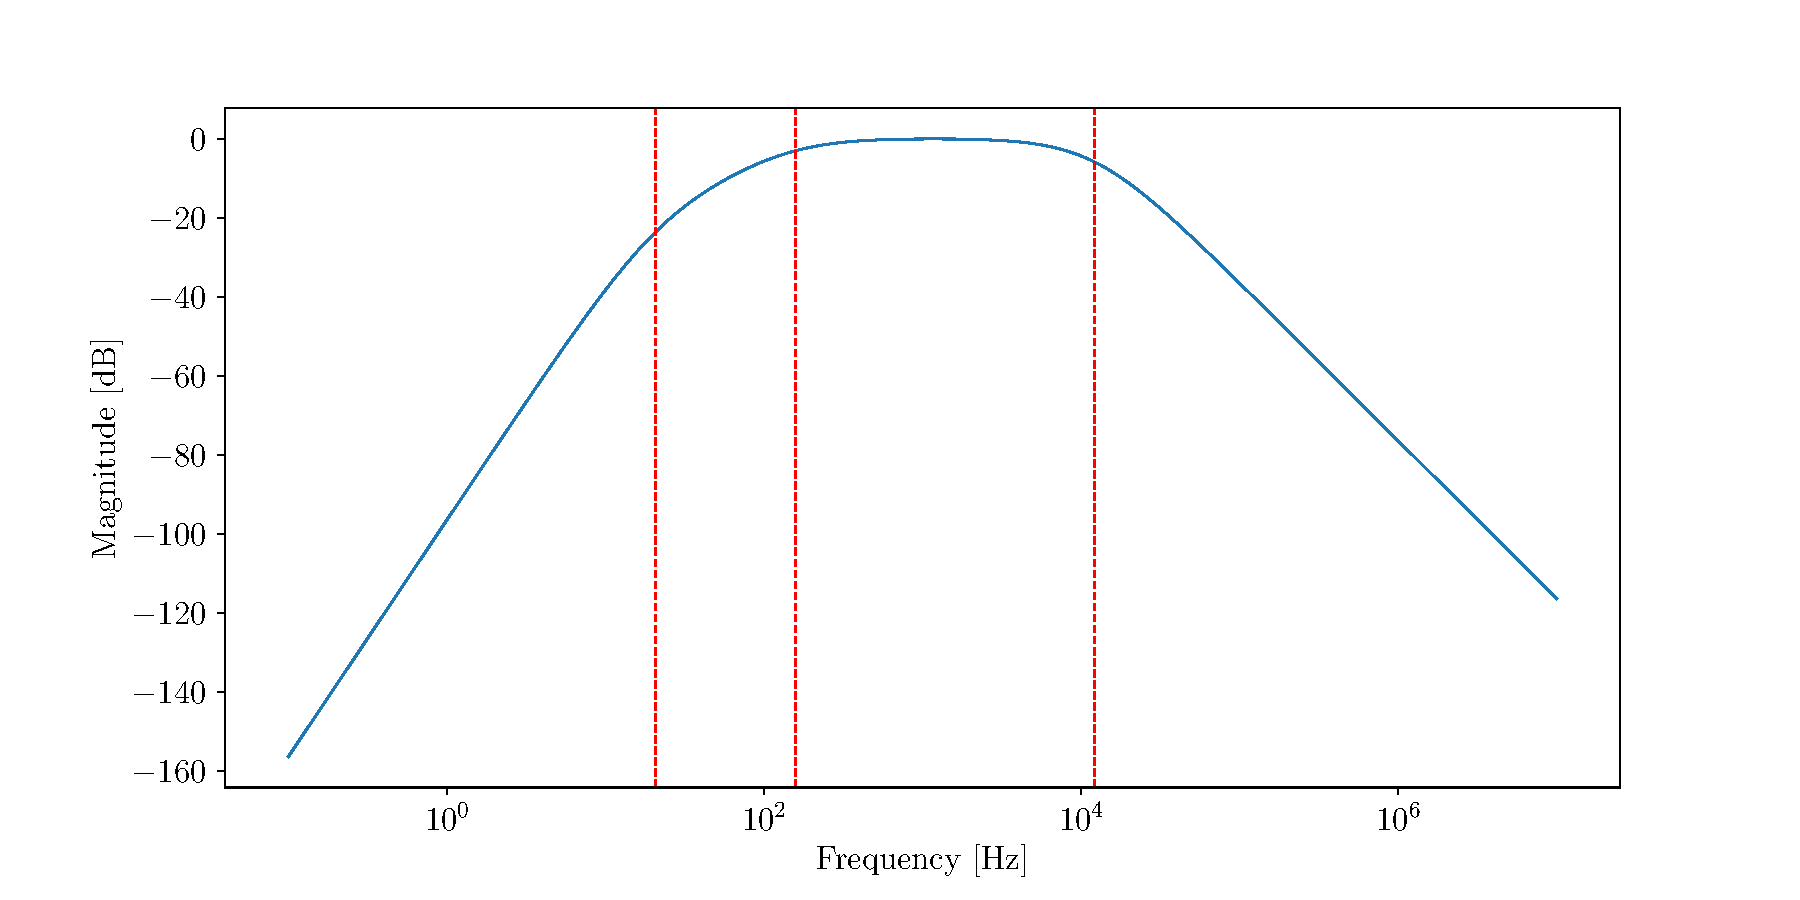
\includegraphics[height=4.2cm]{../figs/signal_filtering/bode_mag.pdf}};
\end{tikzpicture}

\end{frame}

%---------------------------------------------------------------%

\stepcounter{sectionframecount}
\begin{frame}[t]{Filter Application: ODE Approach}
\vspace{-10pt}
Common filtering techniques not suitable for our unstructured grid.

\vspace{8pt}
Convert transfer function in complex frequency domain:

\begin{equation}
  \tilde{P}(s) =P(s)\dfrac{K^{1/3}}{(s+a)^2}\dfrac{K^{1/3}s^2}{(s+c)^2}\dfrac{K^{1/3}s}{(s+b)},
\end{equation}

to a \textbf{system of ODE's} in the time domain (to solve in \textit{ground} boundary):

\begin{equation}
  \dfrac{d\bar{u}}{dt} =
      \begin{pmatrix}
          0 & 1 & 0 & 0 & 0\\
          -a^2 & -2a & 0 & 0 & 0\\
          0 & 0 & 0 & 1 & 0\\
          -K^{1/3}a^2 & -2K^{1/3}a & -c^2 & -2c & 0\\
          0 & 0 & 0 &K^{1/3} & -b
      \end{pmatrix}
      \bar{u}
      +
      \begin{pmatrix}
          0 \\
          K^{1/3}p(t)\\
          0\\
          K^{2/3}p(t)\\
          0
      \end{pmatrix},
  \end{equation}
where $\bar{u}=(u_0,u_1,u_2,u_3,\tilde{p})^T$, with homogeneous initial conditions.
\end{frame}

%=============================================================================%
%=============================================================================%
%=============================================================================%
% FEM Discretization and Output Error Estimation

% TODO: Remove FEM part from here (as it will be with shock capturing)
% TODO: Combine with mesh adaptation

\begin{frame}[plain]
  \vfill
  \centering
  {\usebeamerfont{title}\usebeamercolor[fg]{title}FEM Discretization and Output Error Estimation}
  \vfill
\end{frame}

\section{FEM Discretization and Output Error Estimation}

\setsectionframes{7}

%---------------------------------------------------------------%

% TODO: just say is a CG type FEM
% TODO: can a discontinuous subscale is used for stabilization

\stepcounter{sectionframecount}
\begin{frame}[t]{Variational Multiscale with Discontinuous Subscales (VMSD) Method}
  % \vspace{pt}
  \textbf{Discretization of $\Omega$:}

  \vspace{5pt}
  $\mathcal{T}_h := \{\kappa\}_{\kappa = 1}^K$ is a triangulation of the domain $\Omega$ into $K$ elements.


  \vspace{10pt}
  \textbf{Propose solution:}

  $\boldsymbol{u}_h := \bar{\boldsymbol{u}}_{h,p} + \boldsymbol{u}_{h,p^\prime}^\prime$, ~~~~$\bar{\boldsymbol{u}}_{h,p} \in \overline{\mathcal{V}}_{h,p}$,~~ $\boldsymbol{u}^\prime_{h,p^\prime} \in \mathcal{V}^\prime_{h,p^\prime}$.

  \vspace{10pt}
  \textbf{VMSD solution spaces:}

  \vspace{-15pt}
  \begin{equation}
    \text{(\textit{Coarse} scale) } \overline{\mathcal{V}}_{h,p} := \{\boldsymbol{v}\in [C^0(\Omega)]^m : \boldsymbol{v}|_\kappa \in [\mathcal{P}^p(\kappa)]^m, \forall \kappa \in \mathcal{T}_h\},
  \end{equation}

  \vspace{-15pt}
  \begin{equation}
    \text{(\textit{Fine} scale) } \mathcal{V}^\prime_{h,p^\prime} := \{\boldsymbol{v}\in [L^2(\Omega)]^m : \boldsymbol{v}|_\kappa \in [\mathcal{P}^{p^\prime}(\kappa)]^m, \forall \kappa \in \mathcal{T}_h\}.
  \end{equation}

\end{frame}

%---------------------------------------------------------------%

% move this after the space time slide

\stepcounter{sectionframecount}
\begin{frame}[t]{Variational Multiscale with Discontinuous Subscales (VMSD) Method}
  \textbf{Weak statement:}

  \vspace{10pt}
  \textbf{Find $(\bar{\boldsymbol{u}}_{h,p}$, $\boldsymbol{u}^\prime_{h,p^\prime}) \in \overline{\mathcal{V}}_{h,p} \times \mathcal{V}^\prime_{h,p^\prime}$ such that:}
  \begin{equation}
    \mathcal{R}(\bar{\boldsymbol{v}}_{h,p},\boldsymbol{v}^\prime_{h,p^\prime};\bar{\boldsymbol{u}}_{h,p},\boldsymbol{u}^\prime_{h,p^\prime}) = 0,~~\forall (\bar{\boldsymbol{v}}_{h,p},\boldsymbol{v}^\prime_{h,p^\prime}) \in \overline{\mathcal{V}}_{h,p} \times \mathcal{V}^\prime_{h,p^\prime}.
    \label{e:multiscale_weak_statement}
  \end{equation}

  \vspace{10pt}
  \textbf{Remarks:}
  \begin{itemize}
    \item $\boldsymbol{u}^\prime_{h,p^\prime}$ DOFs are element-wise decoupled. Thus, they can be static condensed and the total cost becomes the same as a CG method.
    \item For same accuracy requirement, more efficient (less DOFs) than CG and DG.
    \item Adjoint consistent.
  \end{itemize}
\end{frame}

%---------------------------------------------------------------%

\stepcounter{sectionframecount}
\begin{frame}[t]{Output Functional}
  In general, consider output functional of the form:
  \begin{equation}
    \mathcal{J}(\boldsymbol{u}) := \int_{\Omega} g_v(\boldsymbol{u})dV + \int_{\partial \Omega} g_b(\boldsymbol{u})dS.
    \label{e:general_output_functional}
  \end{equation}

We define output error as:

\begin{equation}
  \varepsilon (\boldsymbol{u}_h) := \mathcal{J}(\boldsymbol{u}) - \mathcal{J}(\boldsymbol{u}_h).
\end{equation}

\vspace{8pt}
For general nonlinear problem, the output error can be approximated using the \textbf{dual weighted residual} (DWR) method.

\vspace{10pt}
Needs \textbf{correction}\footnotemark for asymptotically consistent problems.

\footnotetext{B. Couchman 2020}

\end{frame}

%---------------------------------------------------------------%

\stepcounter{sectionframecount}
\begin{frame}[t]{Residual Consistency}
\vspace{-10pt}
  \begin{itemize}
    \item We say the residual form $\mathcal{R}$ is consistent if:
    \begin{equation}
      \mathcal{R}(\boldsymbol{v}_h,\boldsymbol{u}) = 0,~~\forall \boldsymbol{v}_h \in \mathcal{V}_h,
    \end{equation}
    where $\boldsymbol{u}$ is the exact solution.
    \item We say the residual form $\mathcal{R}$ is asymptotically consistent if:

    \begin{equation}
      \mathcal{R}(\boldsymbol{v}_h,\boldsymbol{u}) = \mathcal{O}(h^\alpha),~~\forall \boldsymbol{v}_h \in \mathcal{V}_h,
      \label{e:asymptotic_consistent}
    \end{equation}
    where $\boldsymbol{u}$ is the exact solution, $\alpha>0$, and $h$ is a characteristic element size in $\mathcal{T}_h$.
  \end{itemize}

\vspace{10pt}
In our situation:

\begin{equation}
  \begin{split}
  \mathcal{R}(\boldsymbol{v}_h,&\boldsymbol{u}_h) =
  \mathcal{R}^C(\boldsymbol{v}_h,\boldsymbol{u}_h) + \underbrace{\mathcal{R}^A(\boldsymbol{v}_h,\boldsymbol{u}_h)}_{\text{AV term}}.
  \end{split}
  \label{e:residual_C_A_decomposition}
\end{equation}

\end{frame}

%---------------------------------------------------------------%

% TODO: instead of introducing the mean value linearization, do derivation for linear case
% TODO: then introduce the approximations and the linearization about u_h

\stepcounter{sectionframecount}
\begin{frame}[t]{Dual Problem: Mean Value Linearization}
  We define the mean value linearizations of the residual and output functional as:

  \begin{equation}
     \overline{\mathcal{R}}^\prime [\boldsymbol{u}_h,\boldsymbol{u}](\boldsymbol{v},\boldsymbol{w}) := \int_0^1 \mathcal{R}^\prime[\boldsymbol{u}_h + \theta(\underbrace{\boldsymbol{u}-\boldsymbol{u}_h)}_{\Delta \boldsymbol{u}:=}] (\boldsymbol{v},\boldsymbol{w})~d\theta,
  \end{equation}

  \begin{equation}
      \overline{\mathcal{J}}^\prime [\boldsymbol{u}_h,\boldsymbol{u}](\boldsymbol{w}) := \int_0^1 \mathcal{J}^\prime [\boldsymbol{u}_h + \theta(\boldsymbol{u}-\boldsymbol{u}_h)](\boldsymbol{w})~d\theta.
  \end{equation}

  \vspace{10pt}
  Then, the \textbf{dual} (adjoint) problem is:

  \vspace{10pt}
  Find $\boldsymbol{\psi}^\text{mv} \in \mathcal{W} \cup \mathcal{V}_{h}$ such that:

  \begin{equation}
      \overline{\mathcal{R}}^\prime[\boldsymbol{u}_h,\boldsymbol{u}](\boldsymbol{\psi}^\text{mv},\boldsymbol{w}) - \overline{\mathcal{J}}^\prime[\boldsymbol{u}_h,\boldsymbol{u}](\boldsymbol{w}) = 0, ~~\forall \boldsymbol{w} \in \mathcal{W} \cup \mathcal{V}_h.
  \end{equation}

\end{frame}

%---------------------------------------------------------------%

\stepcounter{sectionframecount}
\begin{frame}[t]{DWR From Mean Value Linearization}
  We start from:
  \begin{equation}
    \begin{split}
        \varepsilon(\boldsymbol{u}_h) = \mathcal{J}(\boldsymbol{u}) - \mathcal{J}(\boldsymbol{u}_h) &=
        -\overline{\mathcal{J}}^\prime[\boldsymbol{u}_h,\boldsymbol{u}](\Delta \boldsymbol{u})\\
        &=-\overline{\mathcal{R}}^\prime[\boldsymbol{u}_h,\boldsymbol{u}_h + \Delta \boldsymbol{u}](\boldsymbol{\psi}^\text{mv},\Delta \boldsymbol{u}).
    \end{split}
    \end{equation}
After some work, we obtain the corrected DWR error expression:

\begin{equation}
  \varepsilon(\boldsymbol{u}_h) = -\Big[\mathcal{R}(\boldsymbol{\psi}^\text{mv},\boldsymbol{u}_h) - \mathcal{R}^A(\boldsymbol{\psi}^\text{mv},\boldsymbol{u})\Big].
  \label{e:dwr_corrected_exact}
\end{equation}

\vspace{10pt}
\textbf{Two issues:}

\begin{itemize}
  \item Primal exact solution $\boldsymbol{u}$ is not available.
  \item The mean value adjoint $\boldsymbol{\psi}^{\text{mv}}$ is not computationally tractable.
\end{itemize}

\end{frame}

%---------------------------------------------------------------%

\stepcounter{sectionframecount}
\begin{frame}[t]{Approximations: DWR Estimate}
  \vspace{-10pt}
  \textbf{First approximation}:

  \begin{equation}
    \mathcal{R}^A(\boldsymbol{\psi}^\text{mv},\boldsymbol{u}) \approx
    \mathcal{R}^A(\boldsymbol{\psi}^\text{mv},\boldsymbol{u}_h),
  \end{equation}
  justified on a shock dominated problem with AV.

  \vspace{5pt}
  \textbf{Second approximation:} Tractable adjoint:

  \vspace{10pt}
  $\boldsymbol{\psi}^\text{mv}$ is approximated with a numerical adjoint $\boldsymbol{\psi}_{\hat{h}}$ defined by\footnotemark:

  Find $\boldsymbol{\psi}_{\hat{h}} \in \mathcal{V}_{\hat{h}}$ such that:

\begin{equation}
  \mathcal{J}^\prime[\boldsymbol{u}_h](\tilde{\boldsymbol{u}}) - \mathcal{R}^\prime[\boldsymbol{u}_h](\boldsymbol{\psi}_{\hat{h}},\tilde{\boldsymbol{u}}) = \mathcal{J}^*(\boldsymbol{\psi}_{\hat{h}}) - \mathcal{R}^*(\tilde{\boldsymbol{u}},\boldsymbol{\psi}_{\hat{h}}),~~\forall \tilde{\boldsymbol{u}} \in \mathcal{V}_{\hat{h}}.
\end{equation}

\vspace{10pt}
\textbf{DWR error estimate:}
\begin{equation}
  \varepsilon(\boldsymbol{u}_h) \approx -\Big[\mathcal{R}(\boldsymbol{\psi}_{\hat{h}},\boldsymbol{u}_h) - \mathcal{R}^A(\boldsymbol{\psi}_{\hat{h}},\boldsymbol{u}_h)\Big].
\end{equation}

\footnotetext{M. Yano and D. L. Darmofal 2012}

\end{frame}

%=============================================================================%
%=============================================================================%
%=============================================================================%
% Output-based Mesh Adaptation

\begin{frame}[plain]
  \vfill
  \centering
  {\usebeamerfont{title}\usebeamercolor[fg]{title}Output-based Mesh Adaptation}
  \vfill
\end{frame}


\section{Output-based Mesh Adaptation}

\setsectionframes{3}

%---------------------------------------------------------------%

\stepcounter{sectionframecount}
\begin{frame}[t]{Continuous Optimization: Mesh-Metric Duality}
\vspace{-10pt}
Want mesh producing the smallest output error indicator:

\begin{equation}
  \hat{\mathcal{T}}_h = \arg \inf_{\mathcal{T}_h \in \mathbb{T}(\Omega)} \mathcal{E}(\mathcal{T}_h),~~~\mathcal{C}(\mathcal{T}_h) < C.
\end{equation}

\textbf{Continuous relaxation}\footnotemark to address intractability of discrete problem.

\begin{equation}
  \hat{\mathcal{M}} = \arg\inf_{\mathcal{M} \in \mathbb{M}(\Omega)} \mathcal{E}(\mathcal{M}),~~~\mathcal{C}(\mathcal{M}) < C
\end{equation}

\begin{tikzpicture}[remember picture,overlay]
  \node[anchor=north east, xshift=-1.1cm, yshift=-5.1cm]
  at (current page.north east) {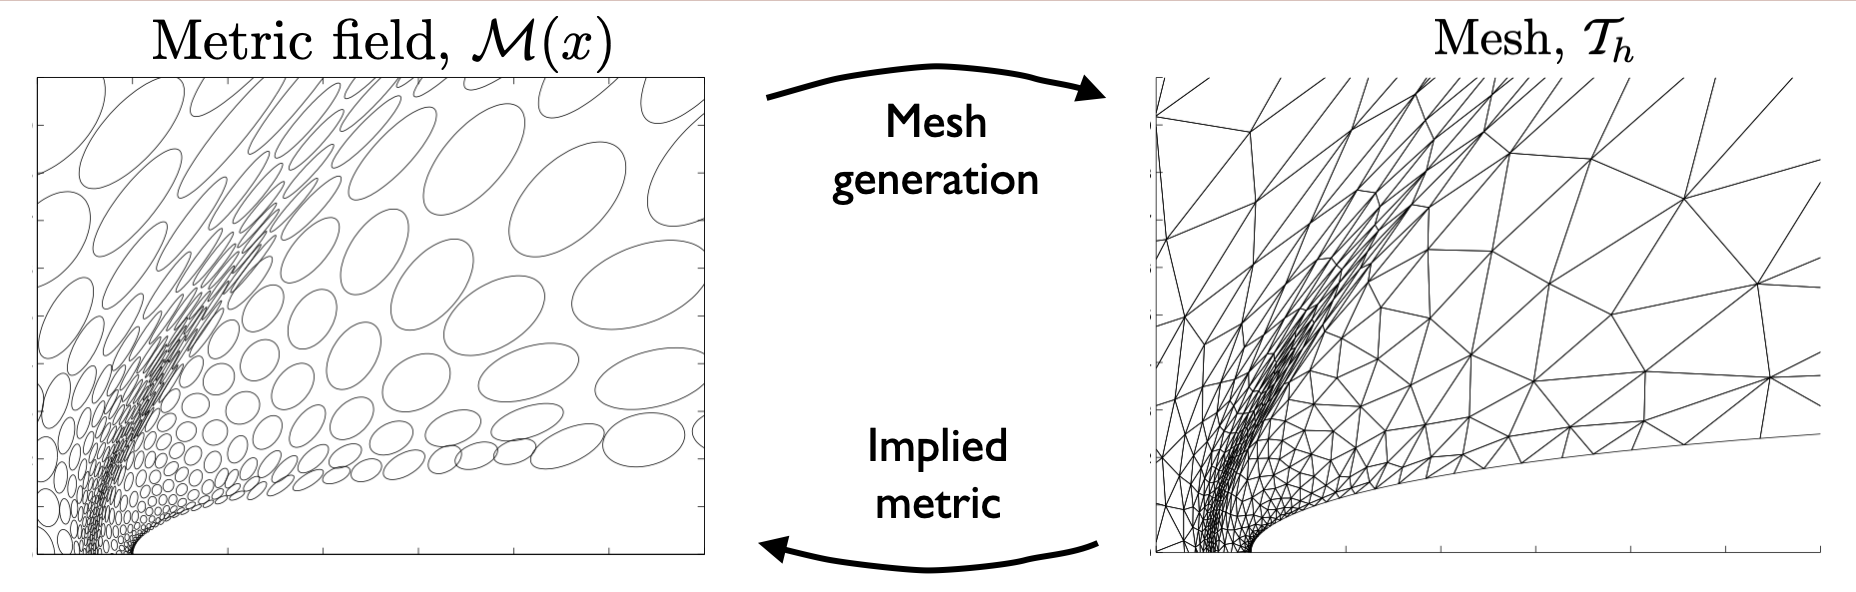
\includegraphics[height=3.4cm]{../figs/mesh_adaptation/mesh_metric_duality.png}};
\end{tikzpicture}

\footnotetext{A. Loseille and F. Alauzet 2011}

\end{frame}

%---------------------------------------------------------------%

% TODO: put emphasis on what we need is model how the error changes when the mesh changes

\stepcounter{sectionframecount}
\begin{frame}[t]{MOESS\footnote{M. Yano and D. L. Darmofal 2012}: Error Sampling and Synthesis}
\vspace{-12pt}
Need model for error indicator $\mathcal{E}(\mathcal{M})$.

Loop over edges in the mesh and compute nodal\footnote{T. Richter and T. Wick 2015} DWR error estimates in \textit{enriched} local patches.

\begin{tikzpicture}[remember picture,overlay]
  \node[anchor=north east, xshift=-2cm, yshift=-2.7cm]
  at (current page.north east) {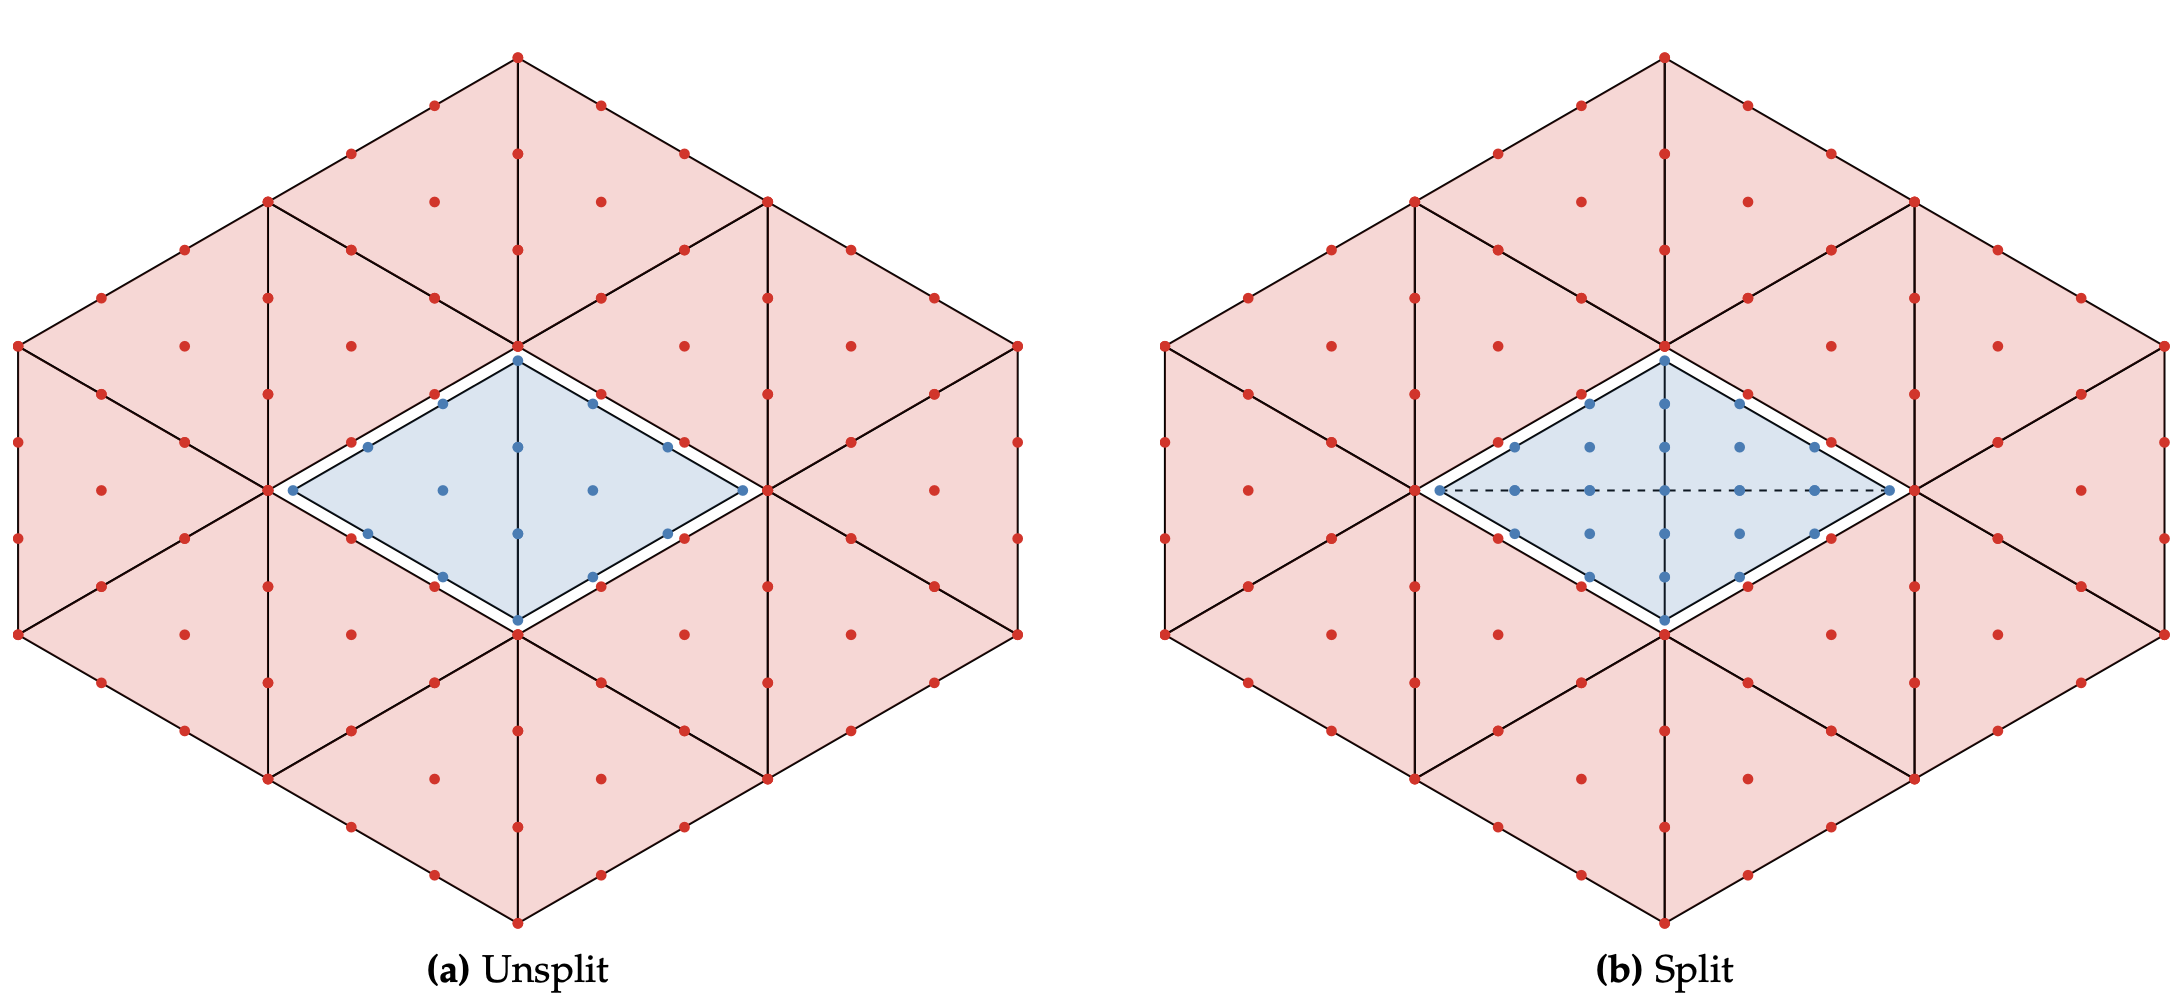
\includegraphics[height=4.0cm]{../figs/mesh_adaptation/local_patches.png}};
\end{tikzpicture}

\vspace{3.1cm}
\begin{equation}
  \text{Nodal error estimate: }\varepsilon_v^\epsilon = -\mathcal{R}_\text{local}(\phi_v \boldsymbol{\psi}_{\hat{h}},\boldsymbol{u}_h^\epsilon) + \mathcal{R}_\text{local}^A(\phi_v\boldsymbol{\psi}_{\hat{h}},\boldsymbol{u}^\epsilon_h),
  \label{e:dwr_est_base_local}
\end{equation}
\vspace{-10pt}
\begin{equation}
  \text{Nodal error indicator: }\eta_v^\epsilon = |\mathcal{R}_\text{local}(\phi_v \boldsymbol{\psi}_{\hat{h}},\boldsymbol{u}_h^\epsilon)| + |\mathcal{R}_\text{local}^A(\phi_v\boldsymbol{\psi}_{\hat{h}},\boldsymbol{u}^\epsilon_h)|.
  \label{e:dwr_ind_base_local}
\end{equation}

\end{frame}

%---------------------------------------------------------------%

% TODO: as said before put this on top

\stepcounter{sectionframecount}
\begin{frame}[t]{Adaptation Cycle}

  \begin{tikzpicture}[remember picture,overlay]
    \node[anchor=north east, xshift=-0.1cm, yshift=-2.7cm]
    at (current page.north east) {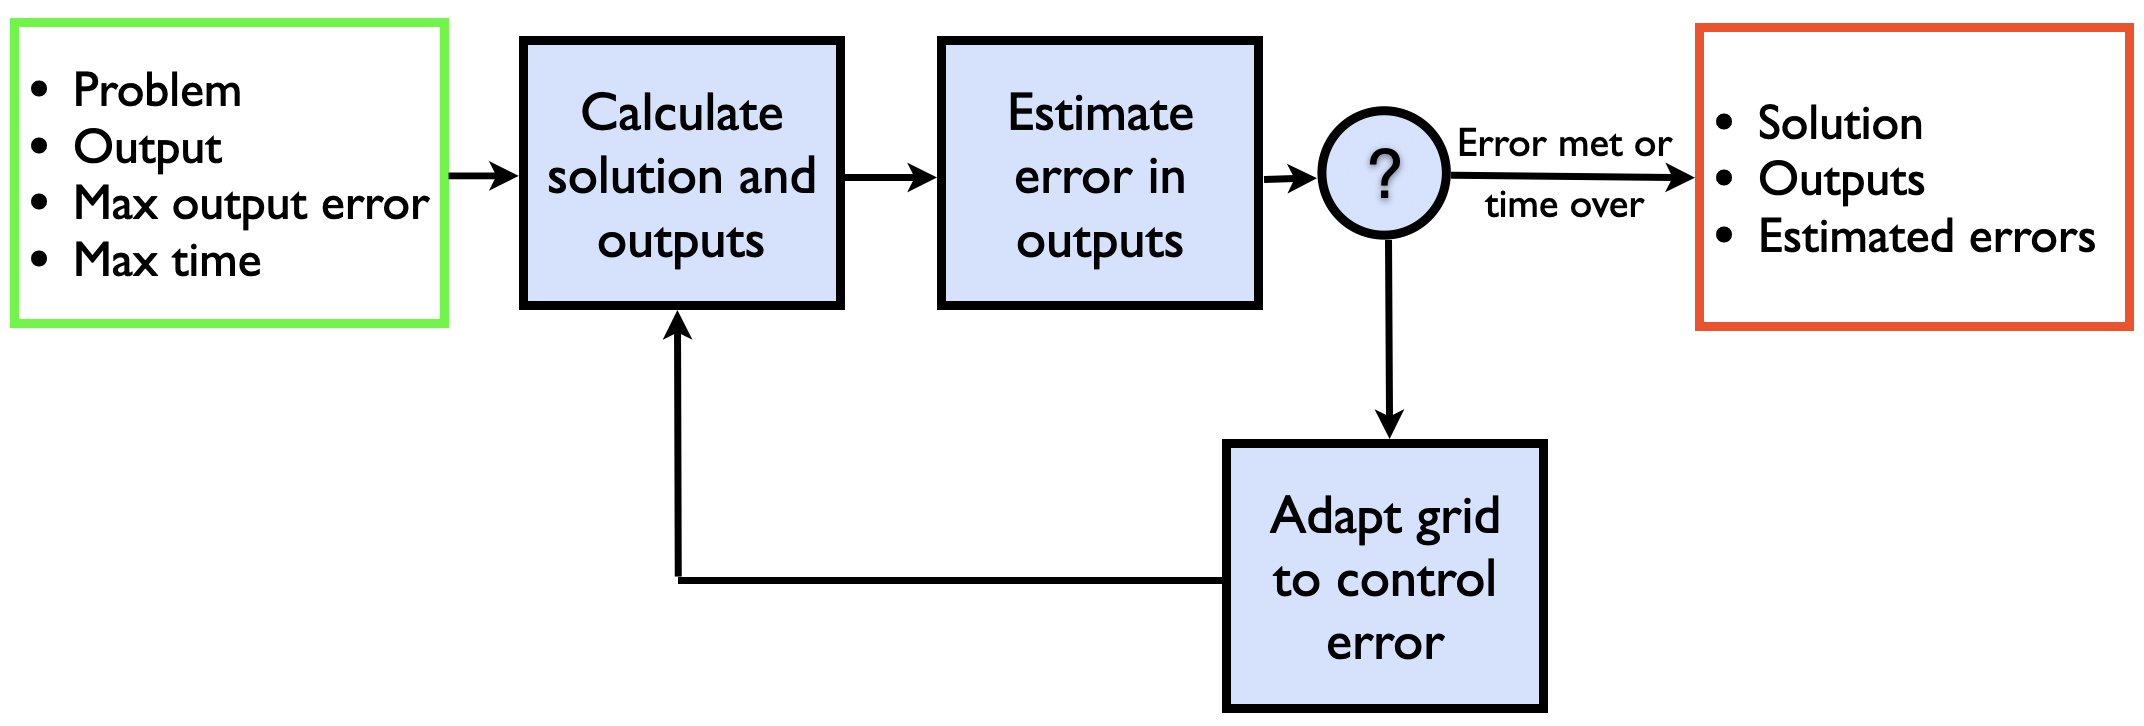
\includegraphics[height=4.2cm]{../figs/mesh_adaptation/adaptation_cycle.png}};
  \end{tikzpicture}

\end{frame}

%=============================================================================%
%=============================================================================%
%=============================================================================%
% Results for Practial Case

\begin{frame}[plain]
  \vfill
  \centering
  {\usebeamerfont{title}\usebeamercolor[fg]{title}Results for Practical Case}
  \vfill
\end{frame}


\section{Results for Practical Case}

\setsectionframes{10}

%---------------------------------------------------------------%

\stepcounter{sectionframecount}
\begin{frame}[t]{Preliminary: Implementation Notes}

\textbf{Software: Solution Adaptive Numerical Simulator (SANS)\footnotemark}
\begin{itemize}
  \item C++ framework to numerically solve partial differential equations.
  \item Extensive use of templates for efficient yet general code.
  \item Supports several CG and DG discretizations, with output-based mesh adaptation.
  \item Automatic differentiation via operator overloading.
  \item MPI parallelization.
  \item Unit testing and continuous integration.
  \item Open source.
\end{itemize}

\footnotetext{Galbraith et. al. 2015}

\end{frame}

%---------------------------------------------------------------%

\stepcounter{sectionframecount}
\begin{frame}[t]{Preliminary: Run Summary}

\begin{enumerate}
  \item \textbf{Set:}
  \begin{itemize}
    \item Case parameters/conditions.
    \item Initial 2D mesh.
    \item Target DOF.
    \item Number of adaptive iterations ($N$).
  \end{itemize}
  \item \textbf{Loop, $i \in \{1,...,N\}$:}
  \begin{itemize}
    \item Extract \textit{ground} boundary and form 1D mesh for filter ODE.
    \item Solve primal problem:
    \begin{itemize}
      \item $[$Burgers system + shock sensor$]$ in 2D mesh.
      \item Filter ODE in 1D mesh (ground boundary).
    \end{itemize}
    \item Solve adjoint problem:
    \begin{itemize}
      \item Adjoint ODE in 1D mesh (ground boundary).
      \item $[$Burgers system + shock sensor$]$ adjoint in 2D mesh.
    \end{itemize}
    \item Nodal error sampling and synthesis.
    \item Adapt mesh.
  \end{itemize}
\end{enumerate}


\end{frame}

%---------------------------------------------------------------%

\stepcounter{sectionframecount}
\begin{frame}[t]{Case Description}
\vspace{-14pt}
\begin{minipage}[t]{0.8\linewidth}
  \begin{itemize}
    \item Airplane Mach number: $M_a = 1.4$.
    \item Airplane altitude: $z_a = 16459.2$ m.
    \item Ground altitude: $110$ m.
    \item Ground reflection factor: $1.9$.
    \item Nearfield signal (initial condition):
  \end{itemize}
\end{minipage}

\begin{tikzpicture}[remember picture,overlay]
  \node[anchor=north east, xshift=-5.5cm, yshift=-4.6cm]
  at (current page.north east) {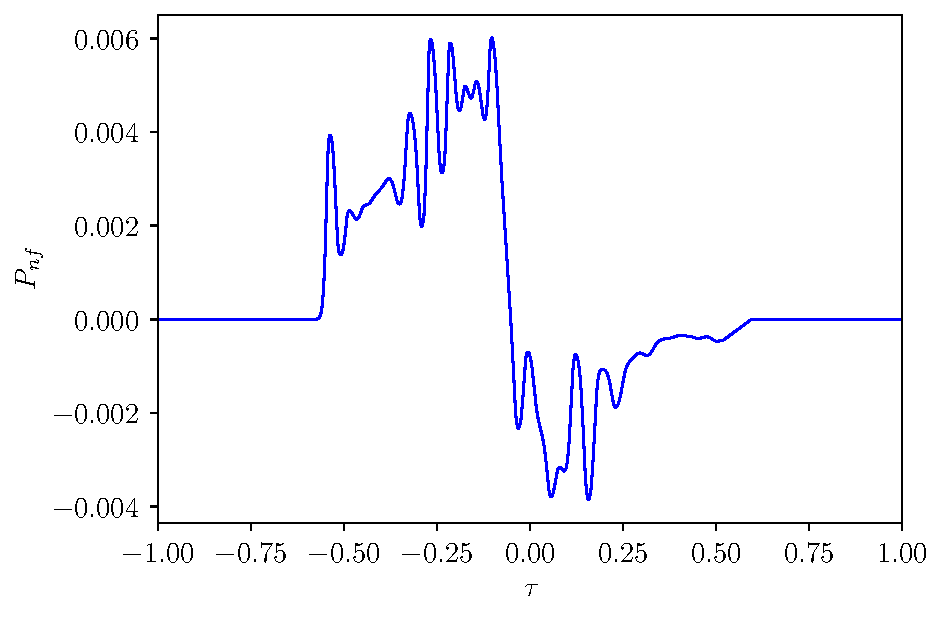
\includegraphics[height=4.4cm]{../figs/SBW3results/nearfield_nondimensional_SBW3_Case2_az0.pdf}};
\end{tikzpicture}

\begin{tikzpicture}[remember picture,overlay]
  % Place the minipage 1cm from the left and 1cm down from the top
  \node[anchor=north east, xshift=0.7cm, yshift=-5.1cm] at (current page.north east) {%
    \begin{minipage}{0.5\textwidth}
      \begin{itemize}
        \item Domain dimensions:
        $\Omega = [-1,2] \times [0,257]$
        \vspace{8pt}
        \item Output for adaptation:
        $\mathcal{J}_{\text{BSEL}} = \int_{\text{ground}} [\tilde{p}(t)]^2~dt$
        \vspace{8pt}
        \item Also for comparison:
        $\mathcal{J}_{p} = \int_{\text{ground}} [p(t)]^2~dt$
      \end{itemize}


    \end{minipage}
  };
\end{tikzpicture}

\begin{tikzpicture}[remember picture,overlay]
  \node[anchor=north east, xshift=-0.2cm, yshift=-1.35cm]
    at (current page.north east) {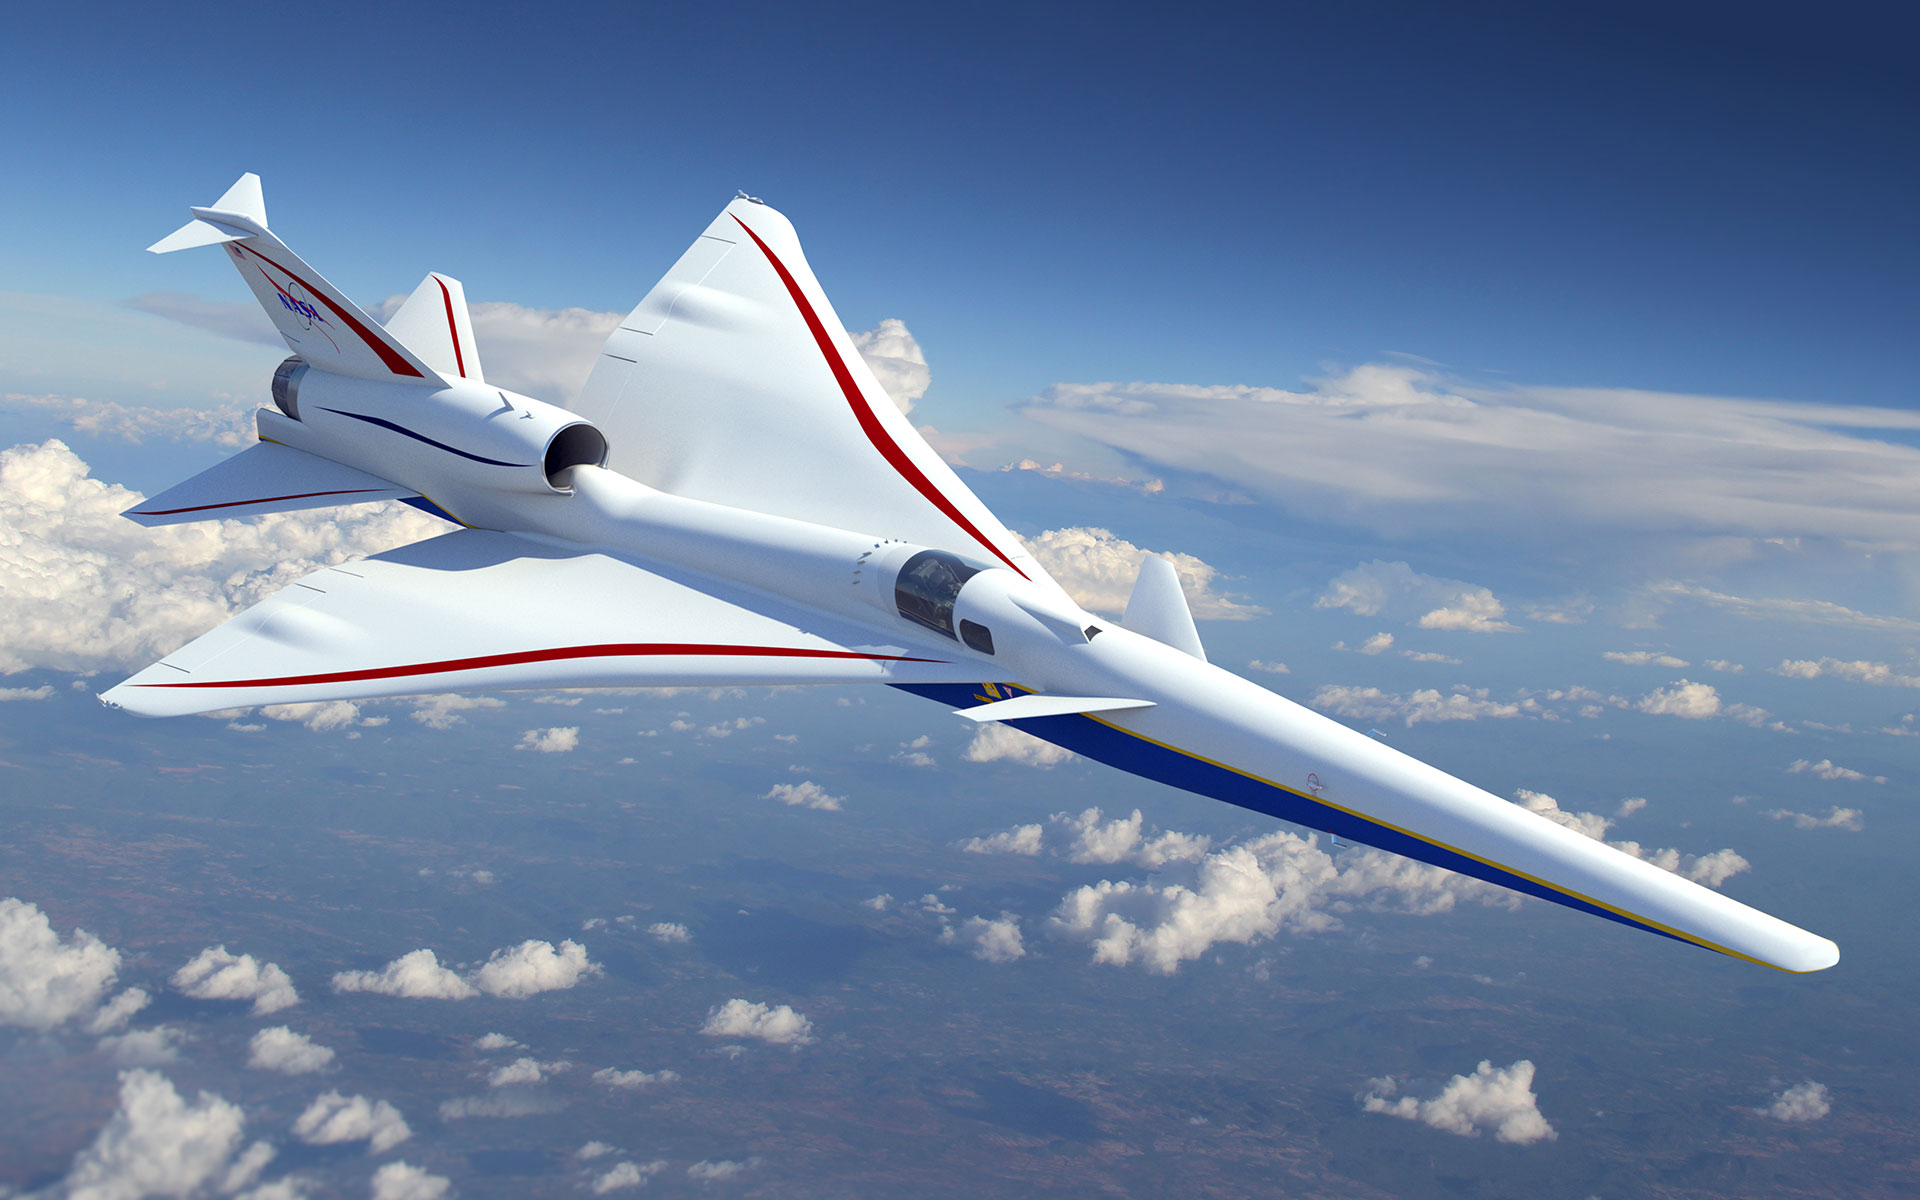
\includegraphics[height=3cm]{../figs/motivation/x59.jpg}};
  \node[anchor=north east, xshift=-2.3cm, yshift=-4.5cm]
    at (current page.north east) {\tiny\color{gray} Source: lockheedmartin.com};
  % https://www.lockheedmartin.com/en-us/products/x-59-quiet-supersonic.html
\end{tikzpicture}

\end{frame}

%---------------------------------------------------------------%

\stepcounter{sectionframecount}
\begin{frame}[t]{Propagation: Pressure Solution}

\begin{tikzpicture}[remember picture,overlay]
  % Place the minipage 1cm from the left and 1cm down from the top
  \node[anchor=north east, xshift=-6.3cm, yshift=-3cm] at (current page.north east) {%
    \begin{minipage}{0.5\textwidth}
    $p=1$

    \end{minipage}
  };
\end{tikzpicture}

\begin{tikzpicture}[remember picture,overlay]
  % Place the minipage 1cm from the left and 1cm down from the top
  \node[anchor=north east, xshift=-6.3cm, yshift=-7cm] at (current page.north east) {%
    \begin{minipage}{0.5\textwidth}
    $p=2$

    \end{minipage}
  };
\end{tikzpicture}

\begin{tikzpicture}[remember picture,overlay]
  \node[anchor=north east, xshift=-6.5cm, yshift=-1.3cm]
  at (current page.north east) {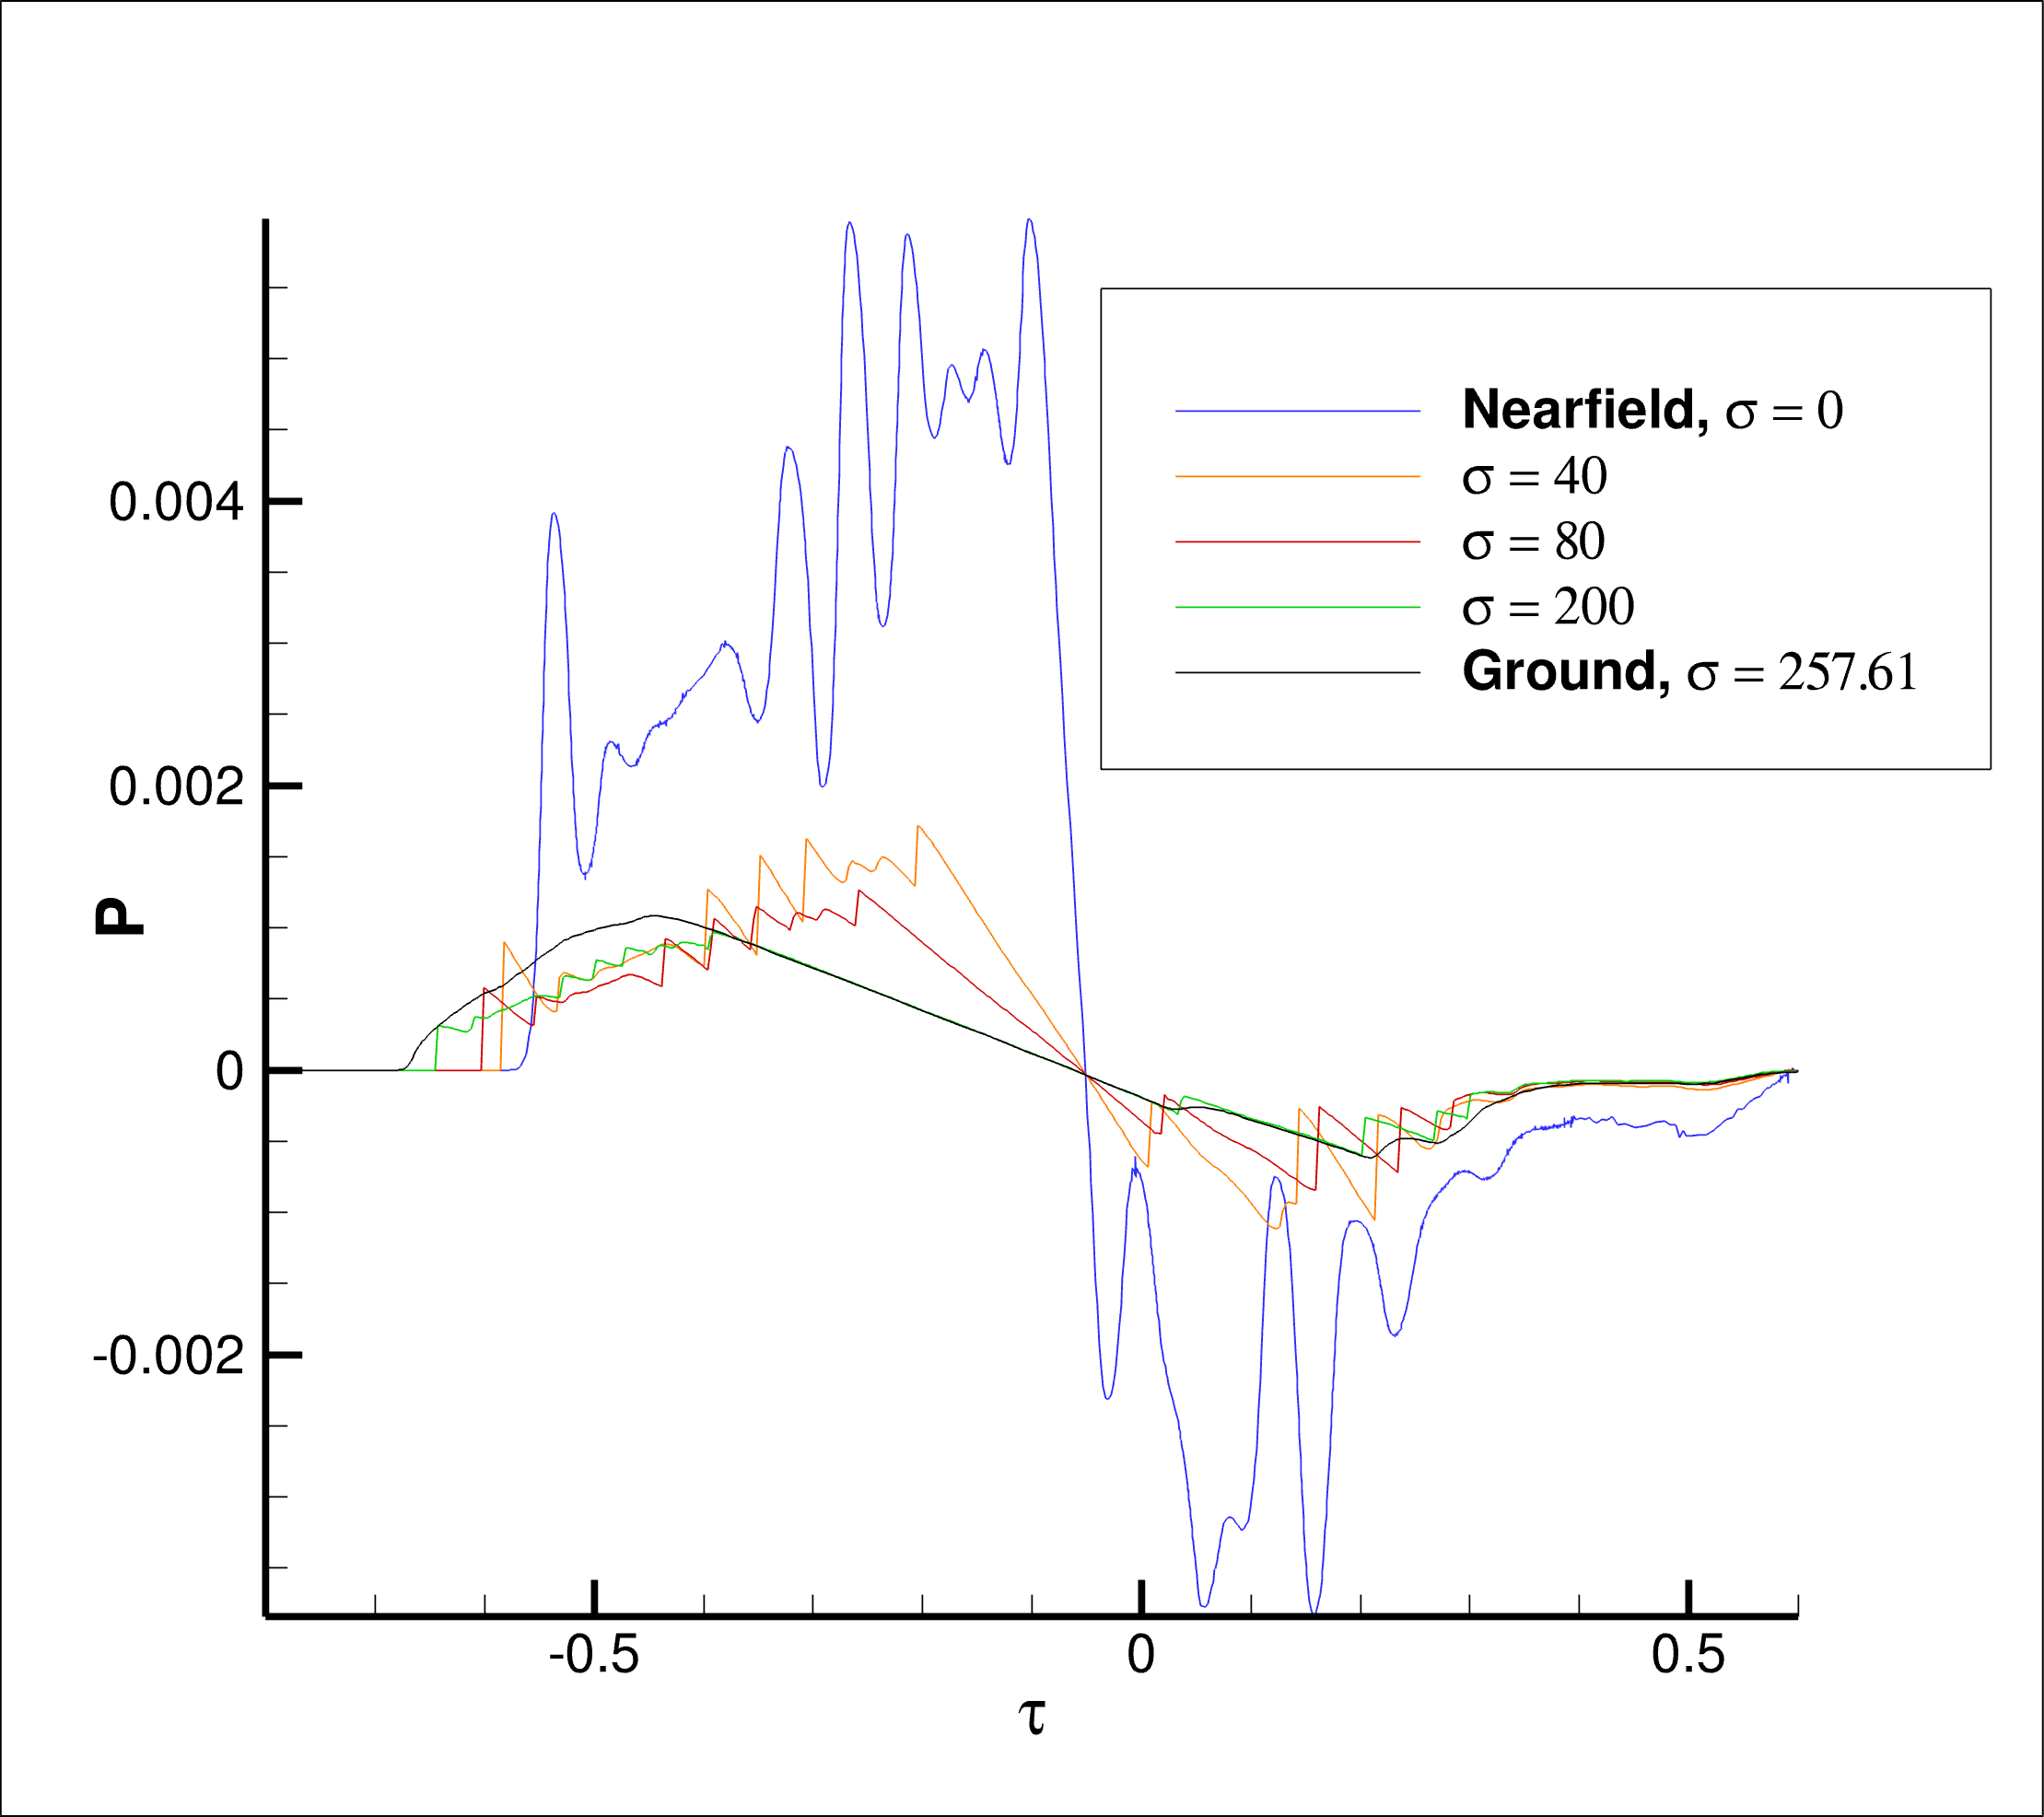
\includegraphics[height=3.9cm]{../figs/SBW3results/sbw3_P1_128K_P_lines.png}};
\end{tikzpicture}

\begin{tikzpicture}[remember picture,overlay]
  \node[anchor=north east, xshift=-1.5cm, yshift=-1.3cm]
  at (current page.north east) {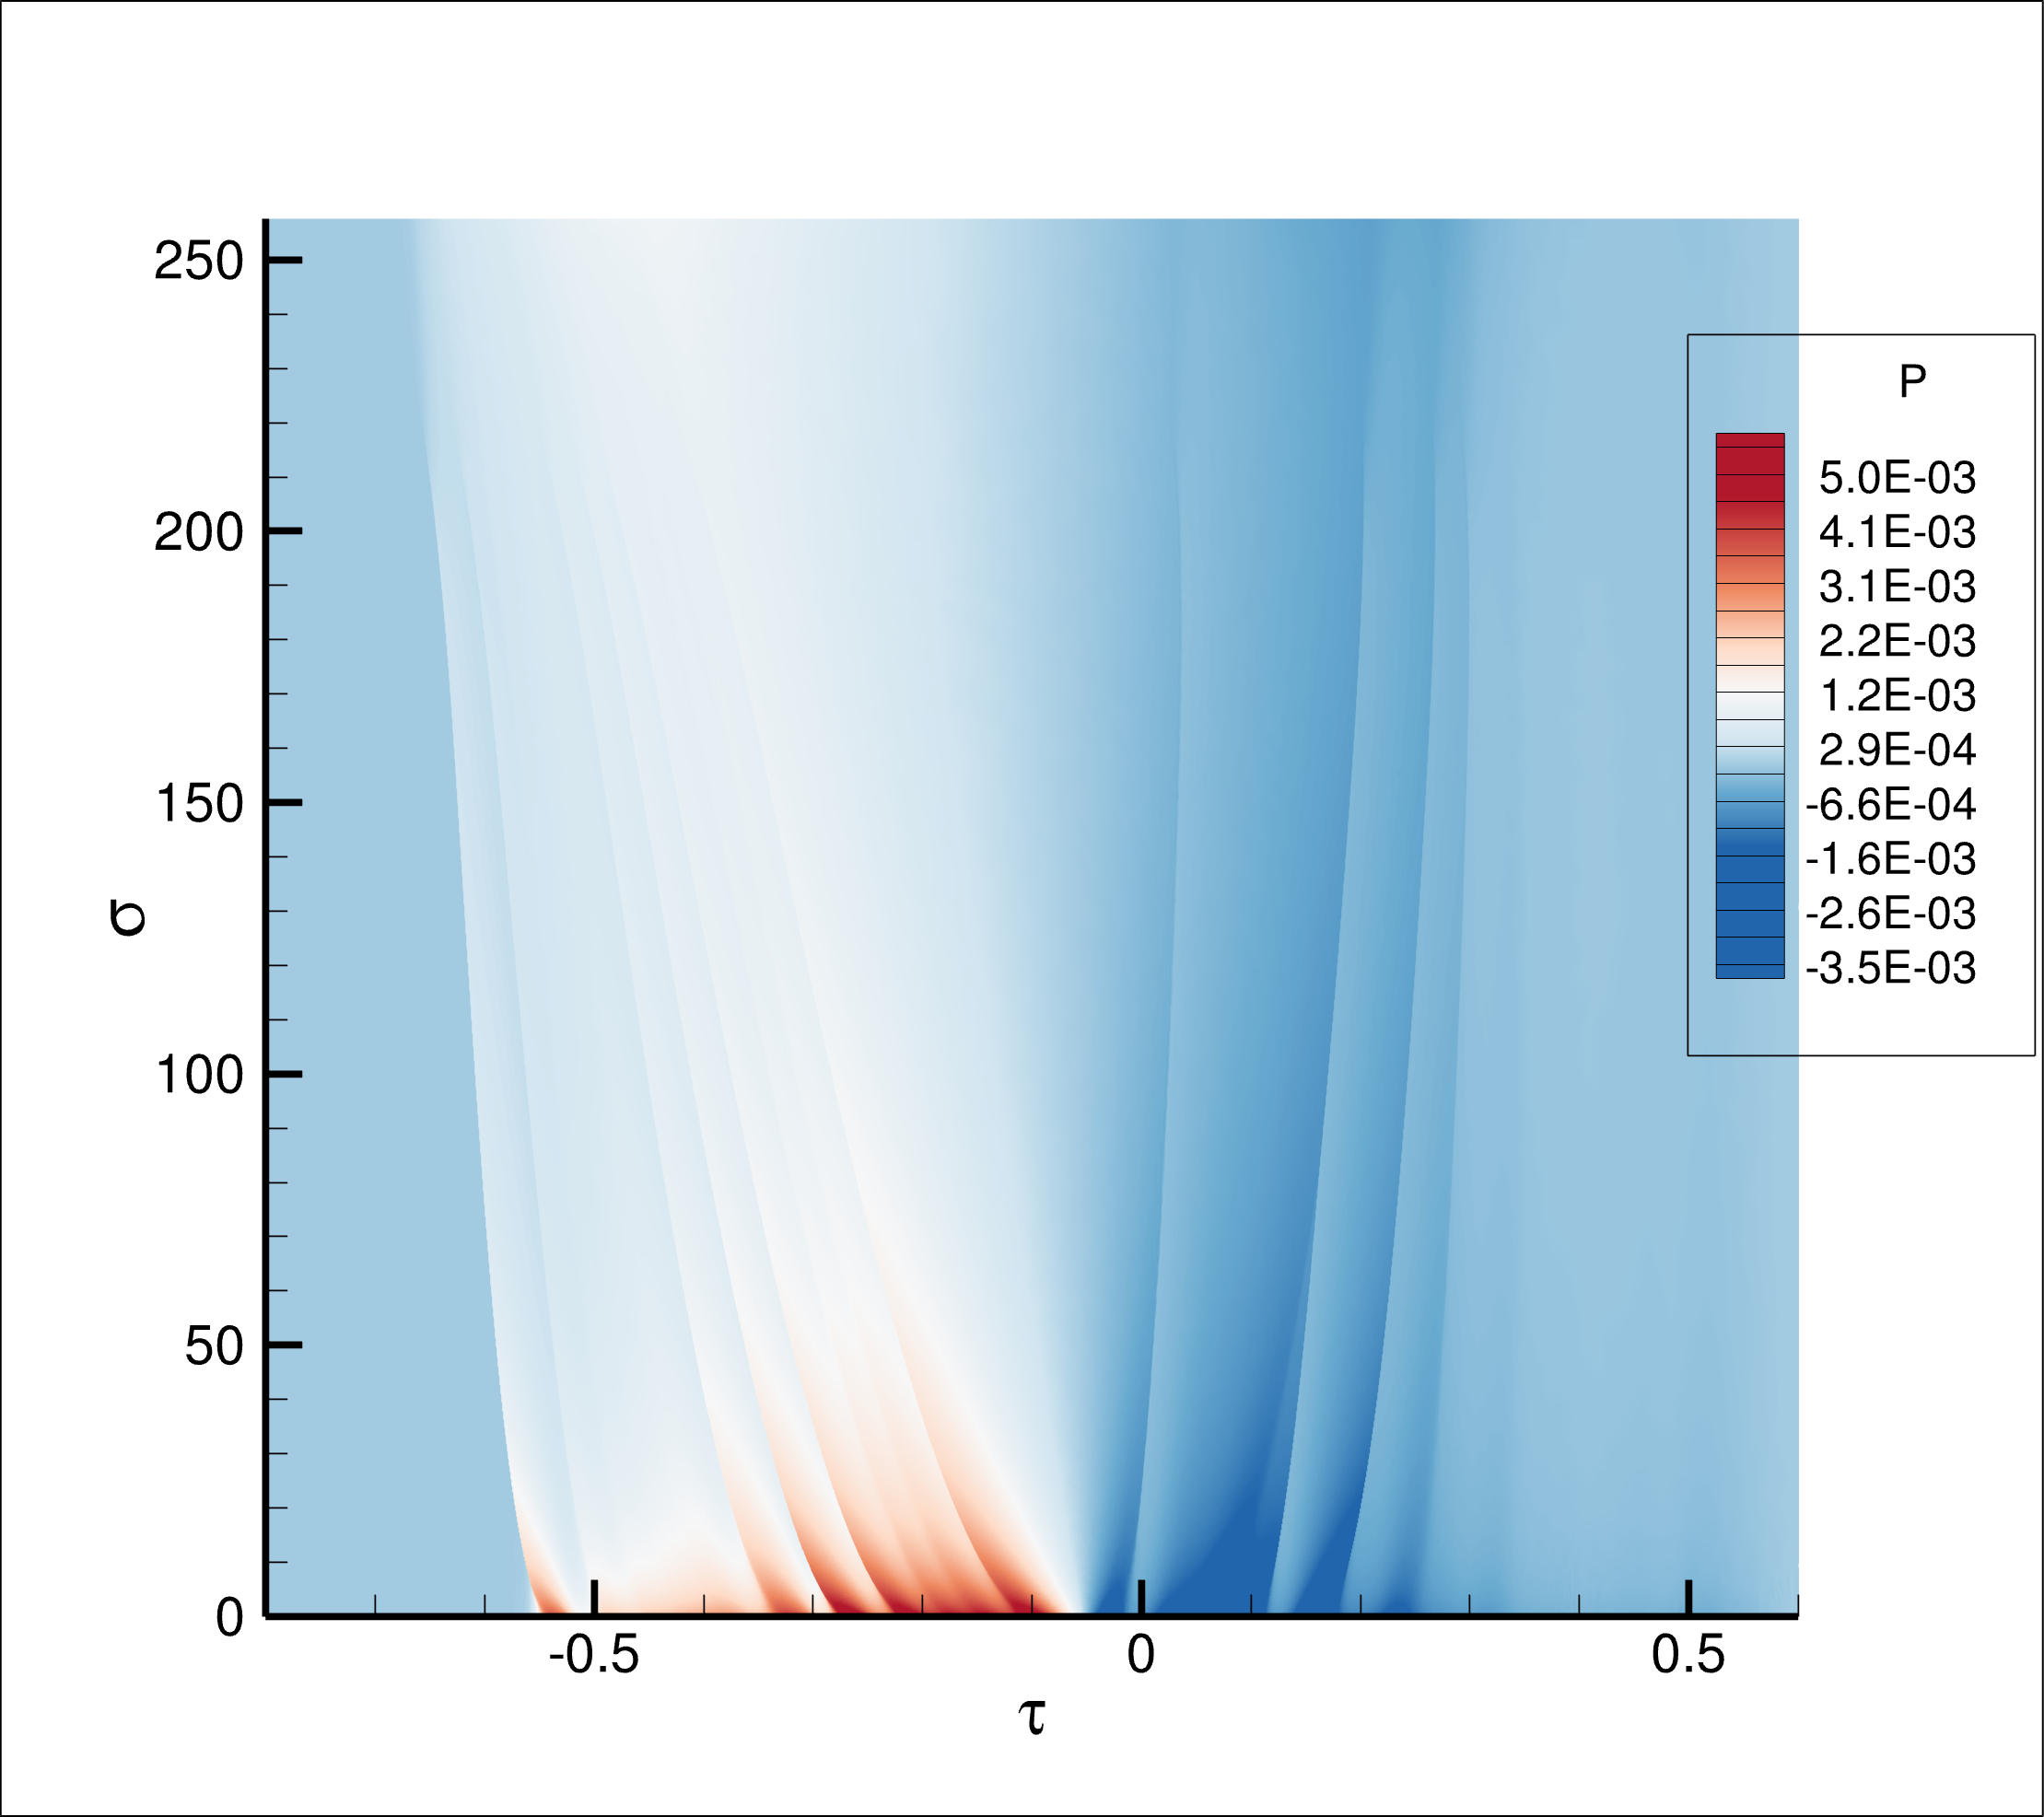
\includegraphics[height=3.9cm]{../figs/SBW3results/sbw3_P1_128K_P_field.png}};
\end{tikzpicture}

\begin{tikzpicture}[remember picture,overlay]
  \node[anchor=north east, xshift=-6.5cm, yshift=-5.3cm]
  at (current page.north east) {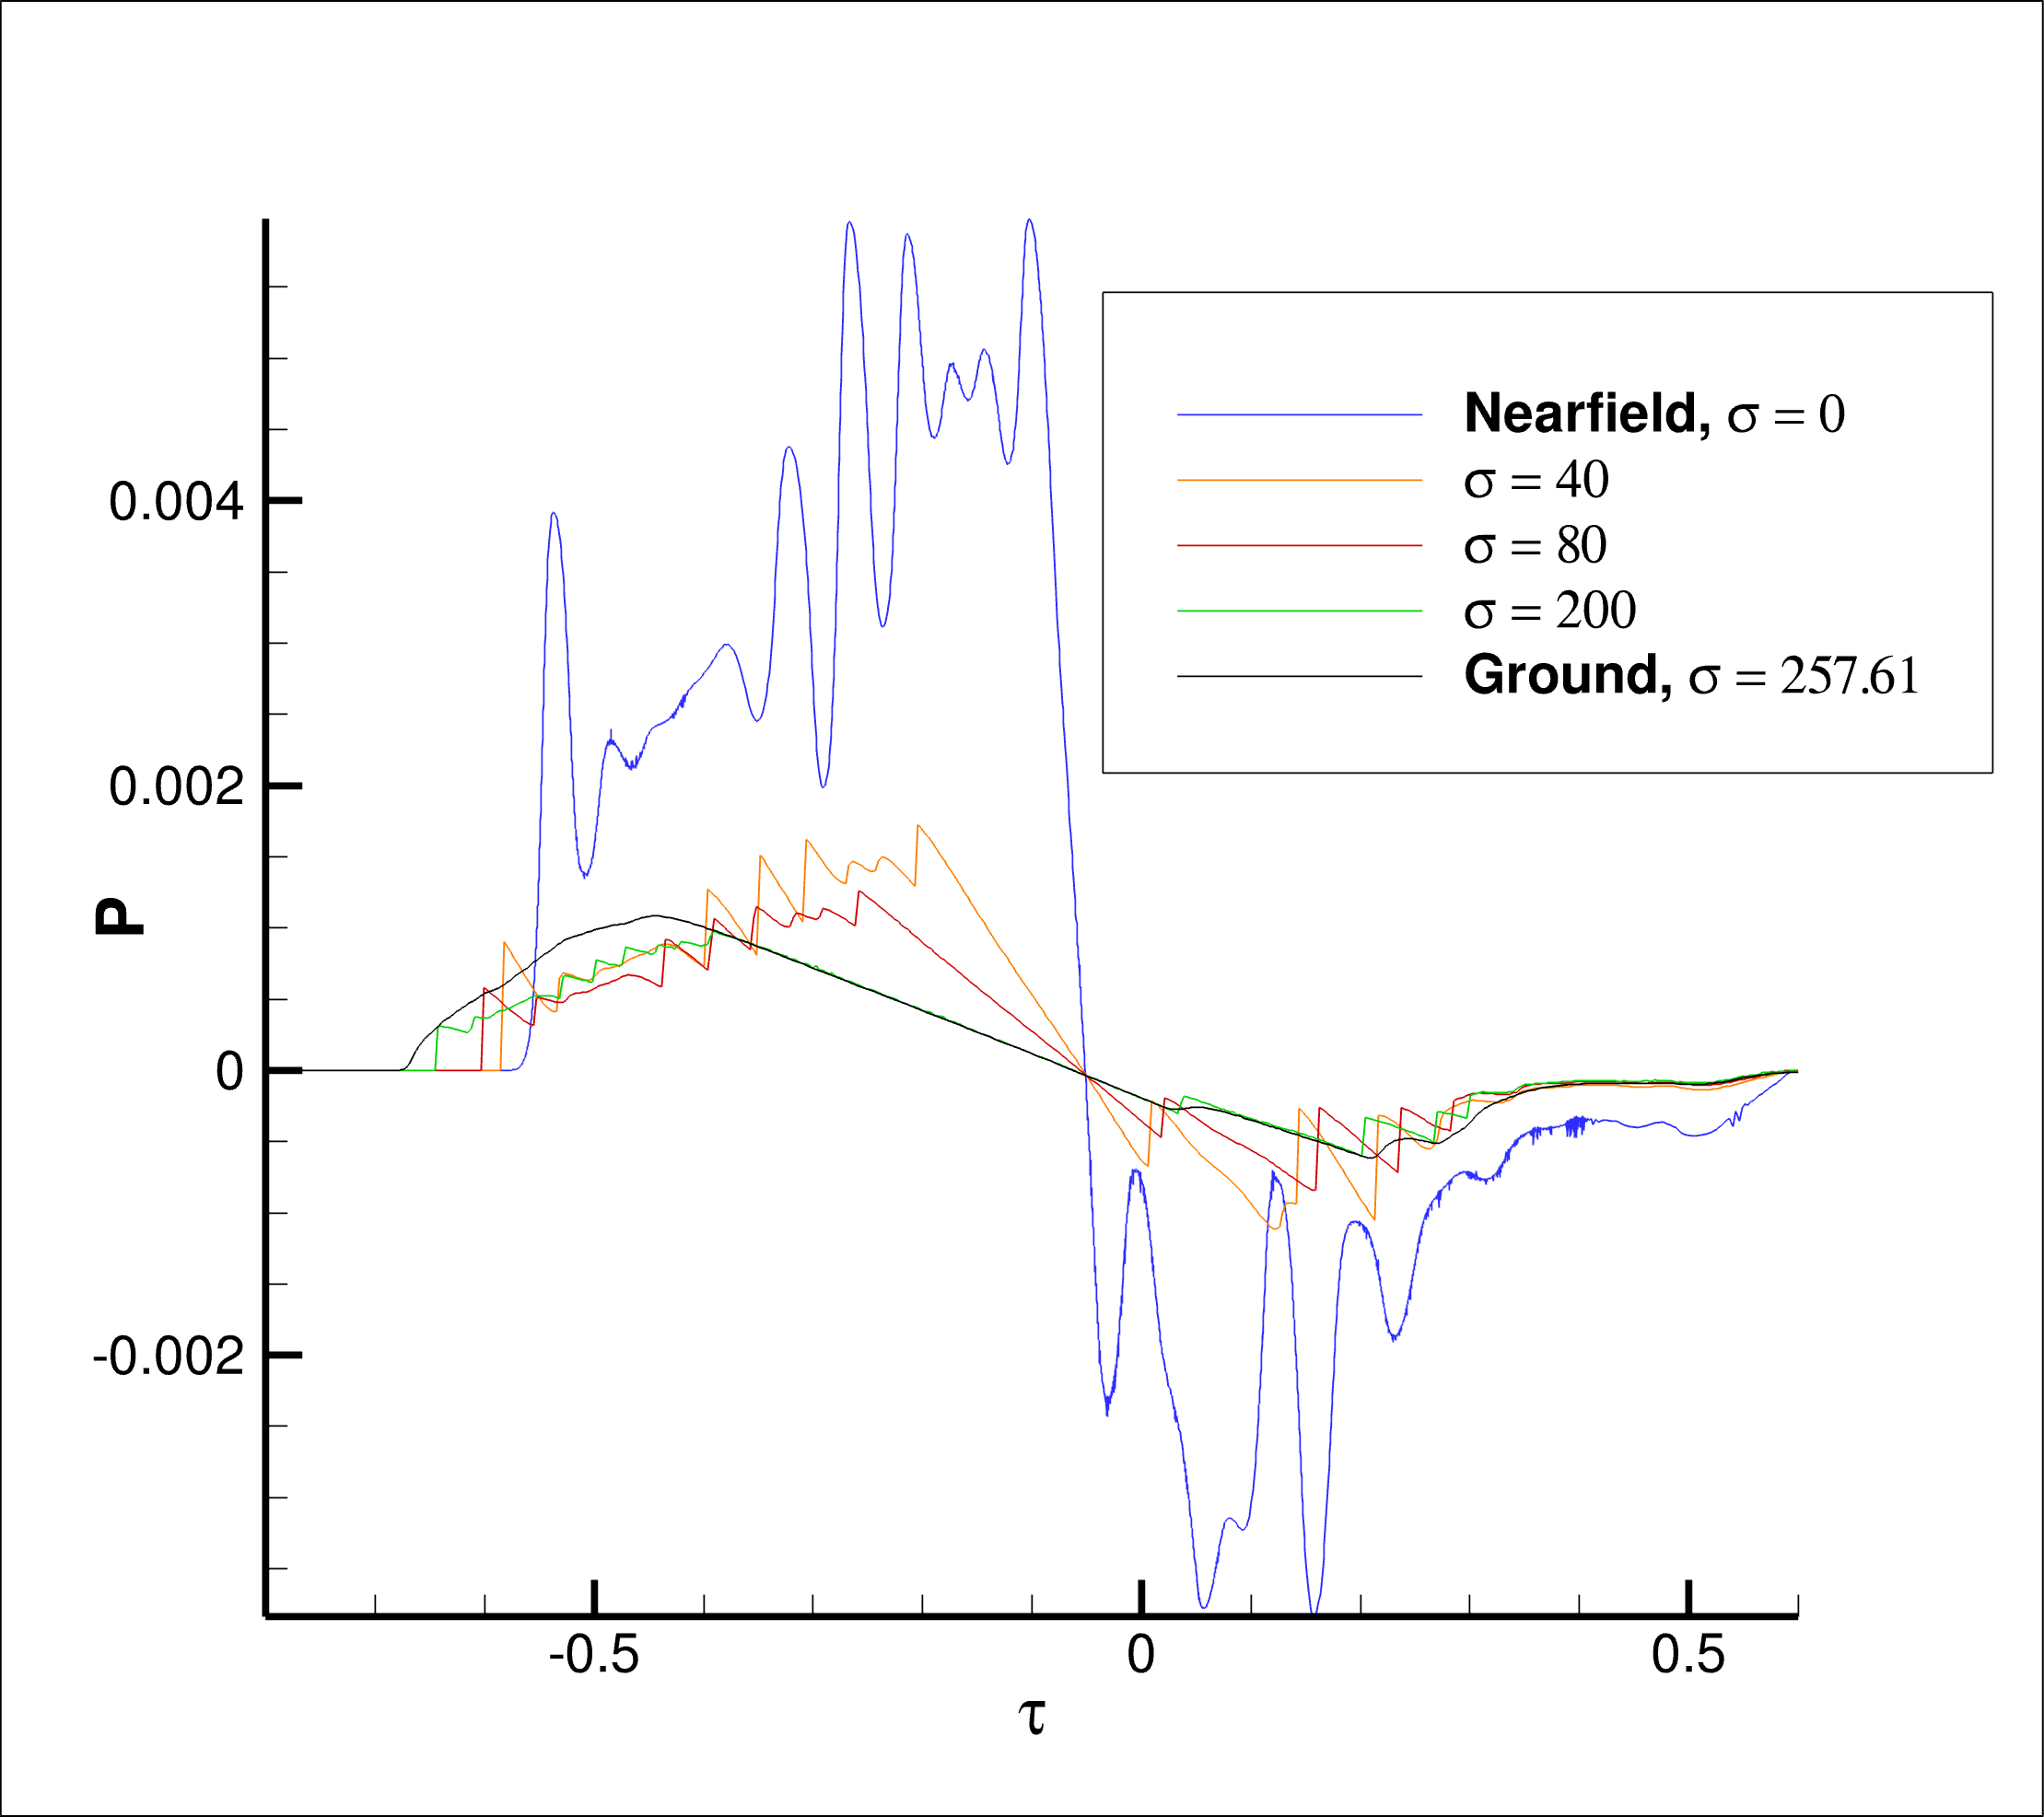
\includegraphics[height=3.9cm]{../figs/SBW3results/sbw3_P2_128K_P_lines.png}};
\end{tikzpicture}

\begin{tikzpicture}[remember picture,overlay]
  \node[anchor=north east, xshift=-1.5cm, yshift=-5.3cm]
  at (current page.north east) {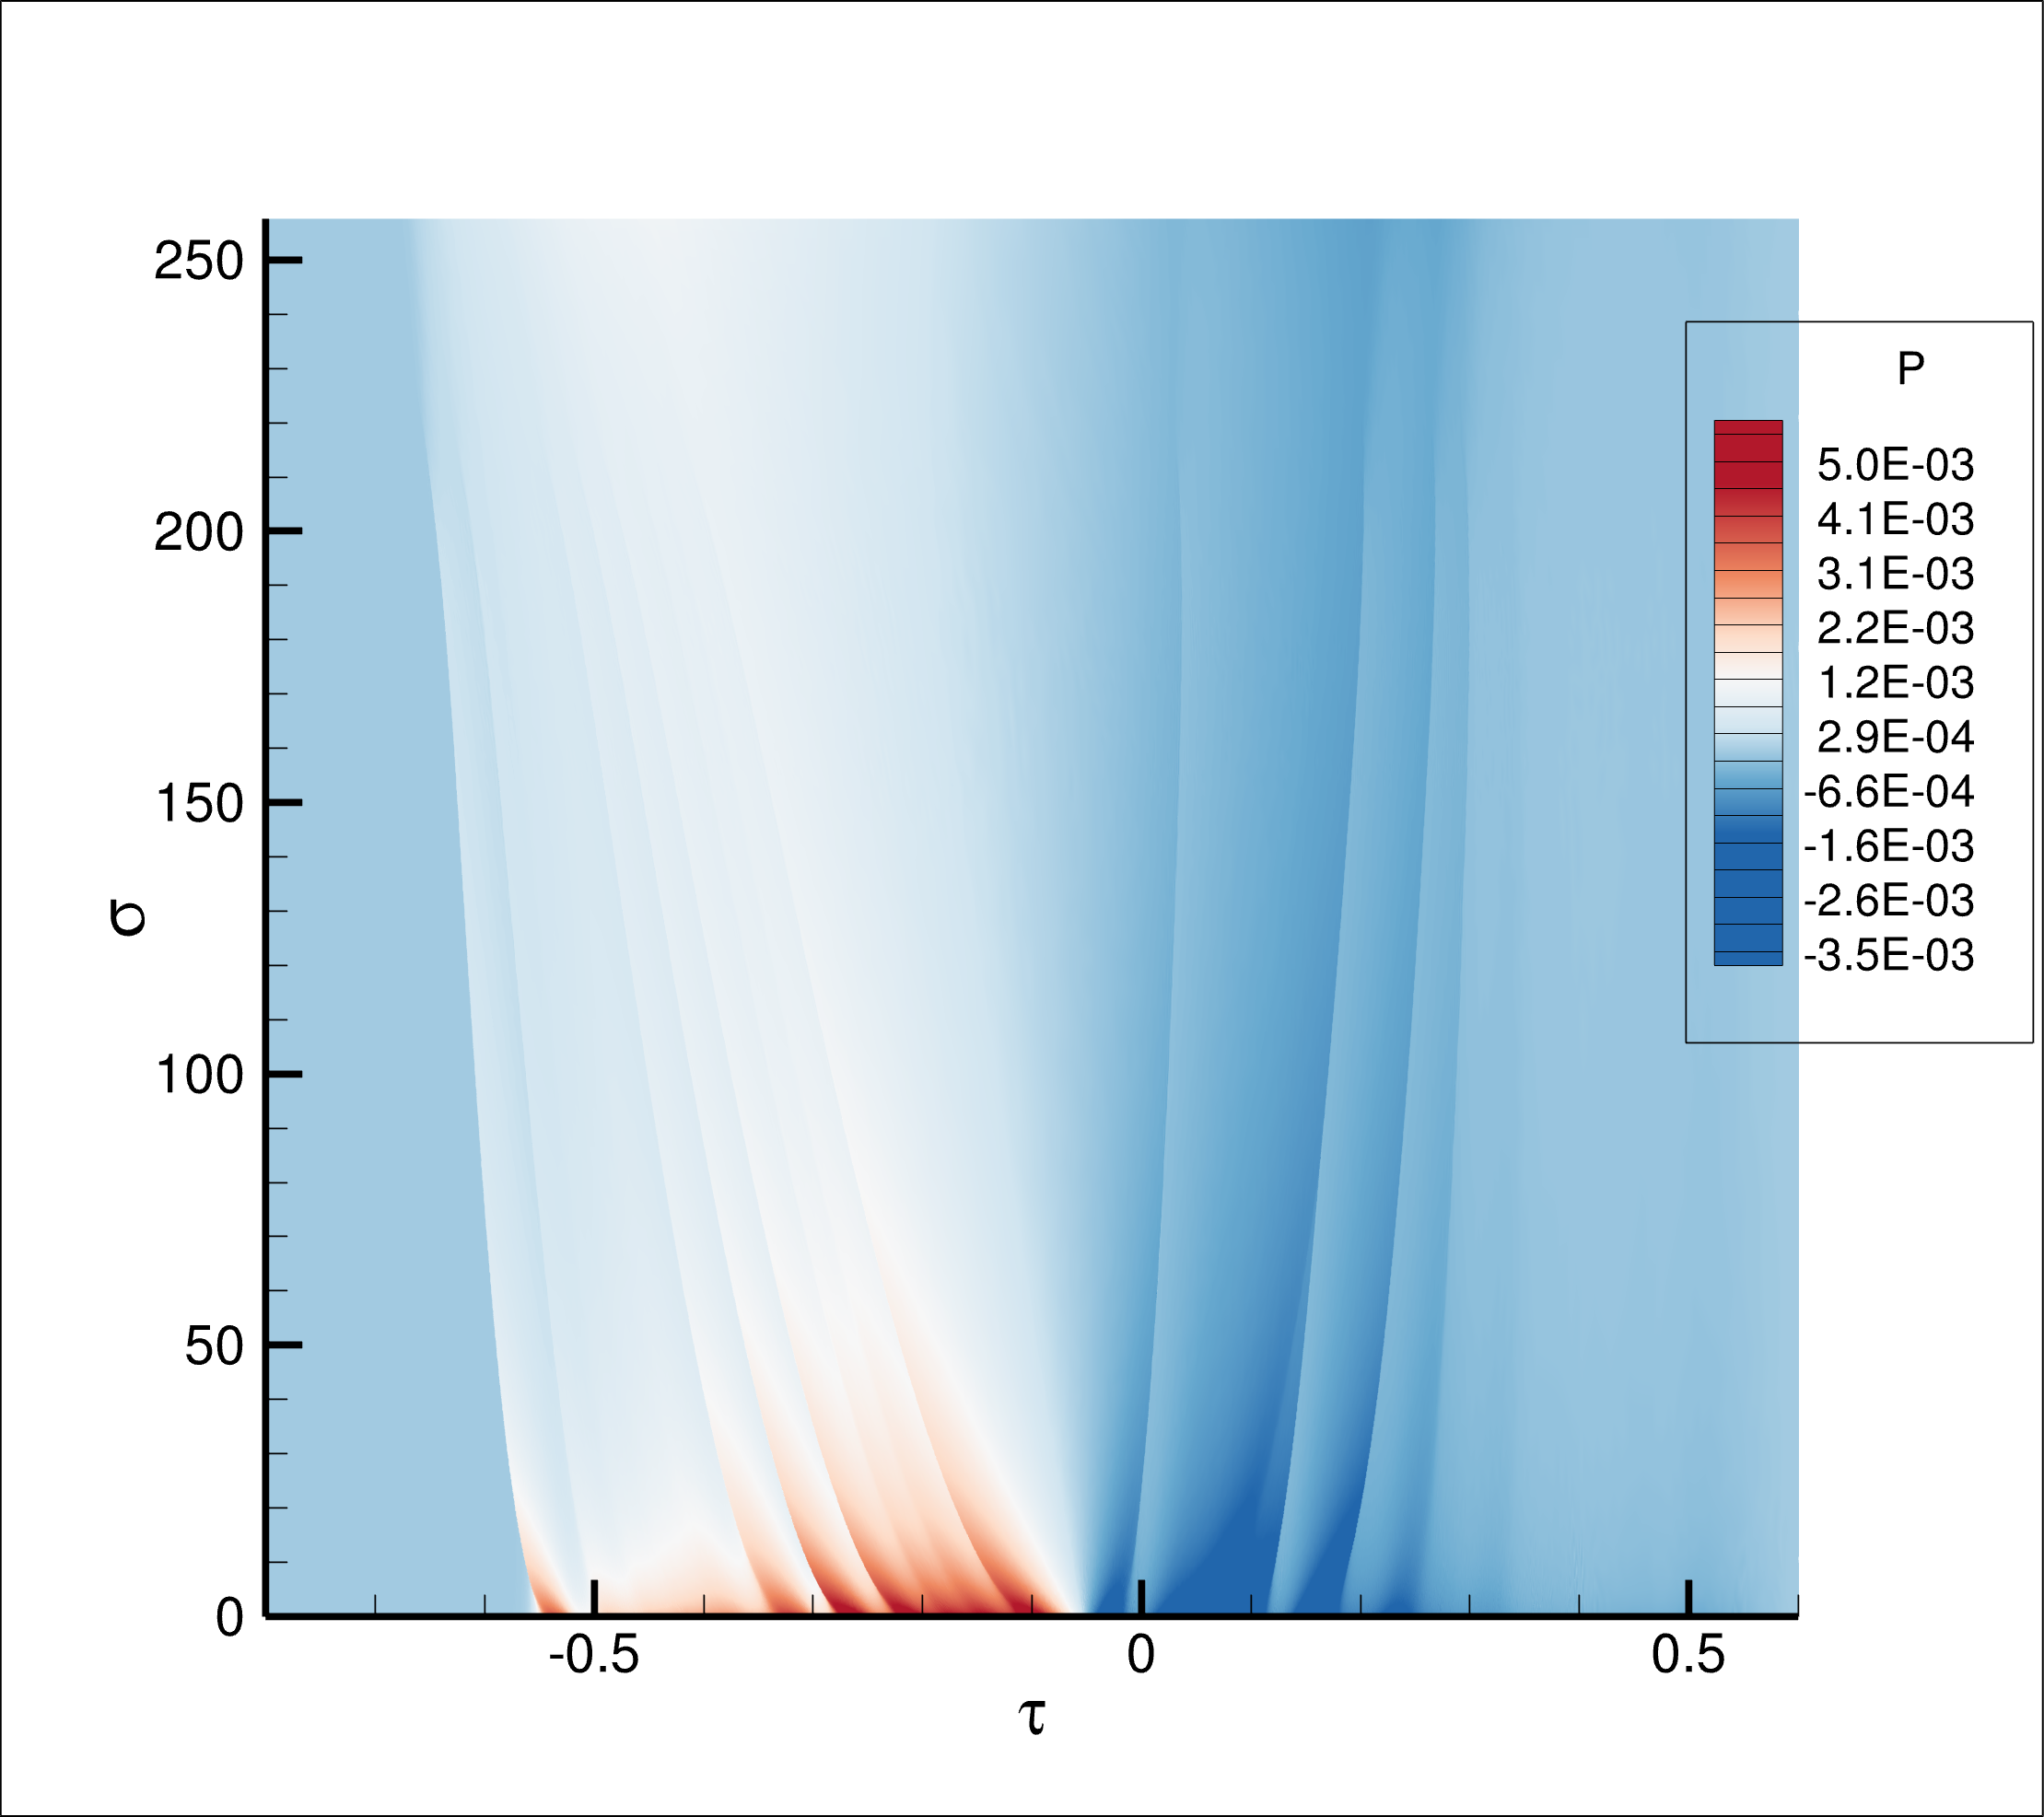
\includegraphics[height=3.9cm]{../figs/SBW3results/sbw3_P2_128K_P_field.png}};
\end{tikzpicture}

\end{frame}

%---------------------------------------------------------------%

\stepcounter{sectionframecount}
\begin{frame}[t]{Propagation: Final Adapted Mesh for 8K Target DOF}

\begin{tikzpicture}[remember picture,overlay]
  % Place the minipage 1cm from the left and 1cm down from the top
  \node[anchor=north east, xshift=-3.5cm, yshift=-1.8cm] at (current page.north east) {%
    \begin{minipage}{0.5\textwidth}
    $p=1$

    \end{minipage}
  };
\end{tikzpicture}

\begin{tikzpicture}[remember picture,overlay]
  % Place the minipage 1cm from the left and 1cm down from the top
  \node[anchor=north east, xshift=2.5cm, yshift=-1.8cm] at (current page.north east) {%
    \begin{minipage}{0.5\textwidth}
    $p=2$

    \end{minipage}
  };
\end{tikzpicture}

\begin{tikzpicture}[remember picture,overlay]
  \node[anchor=north east, xshift=-4.5cm, yshift=-2cm]
  at (current page.north east) {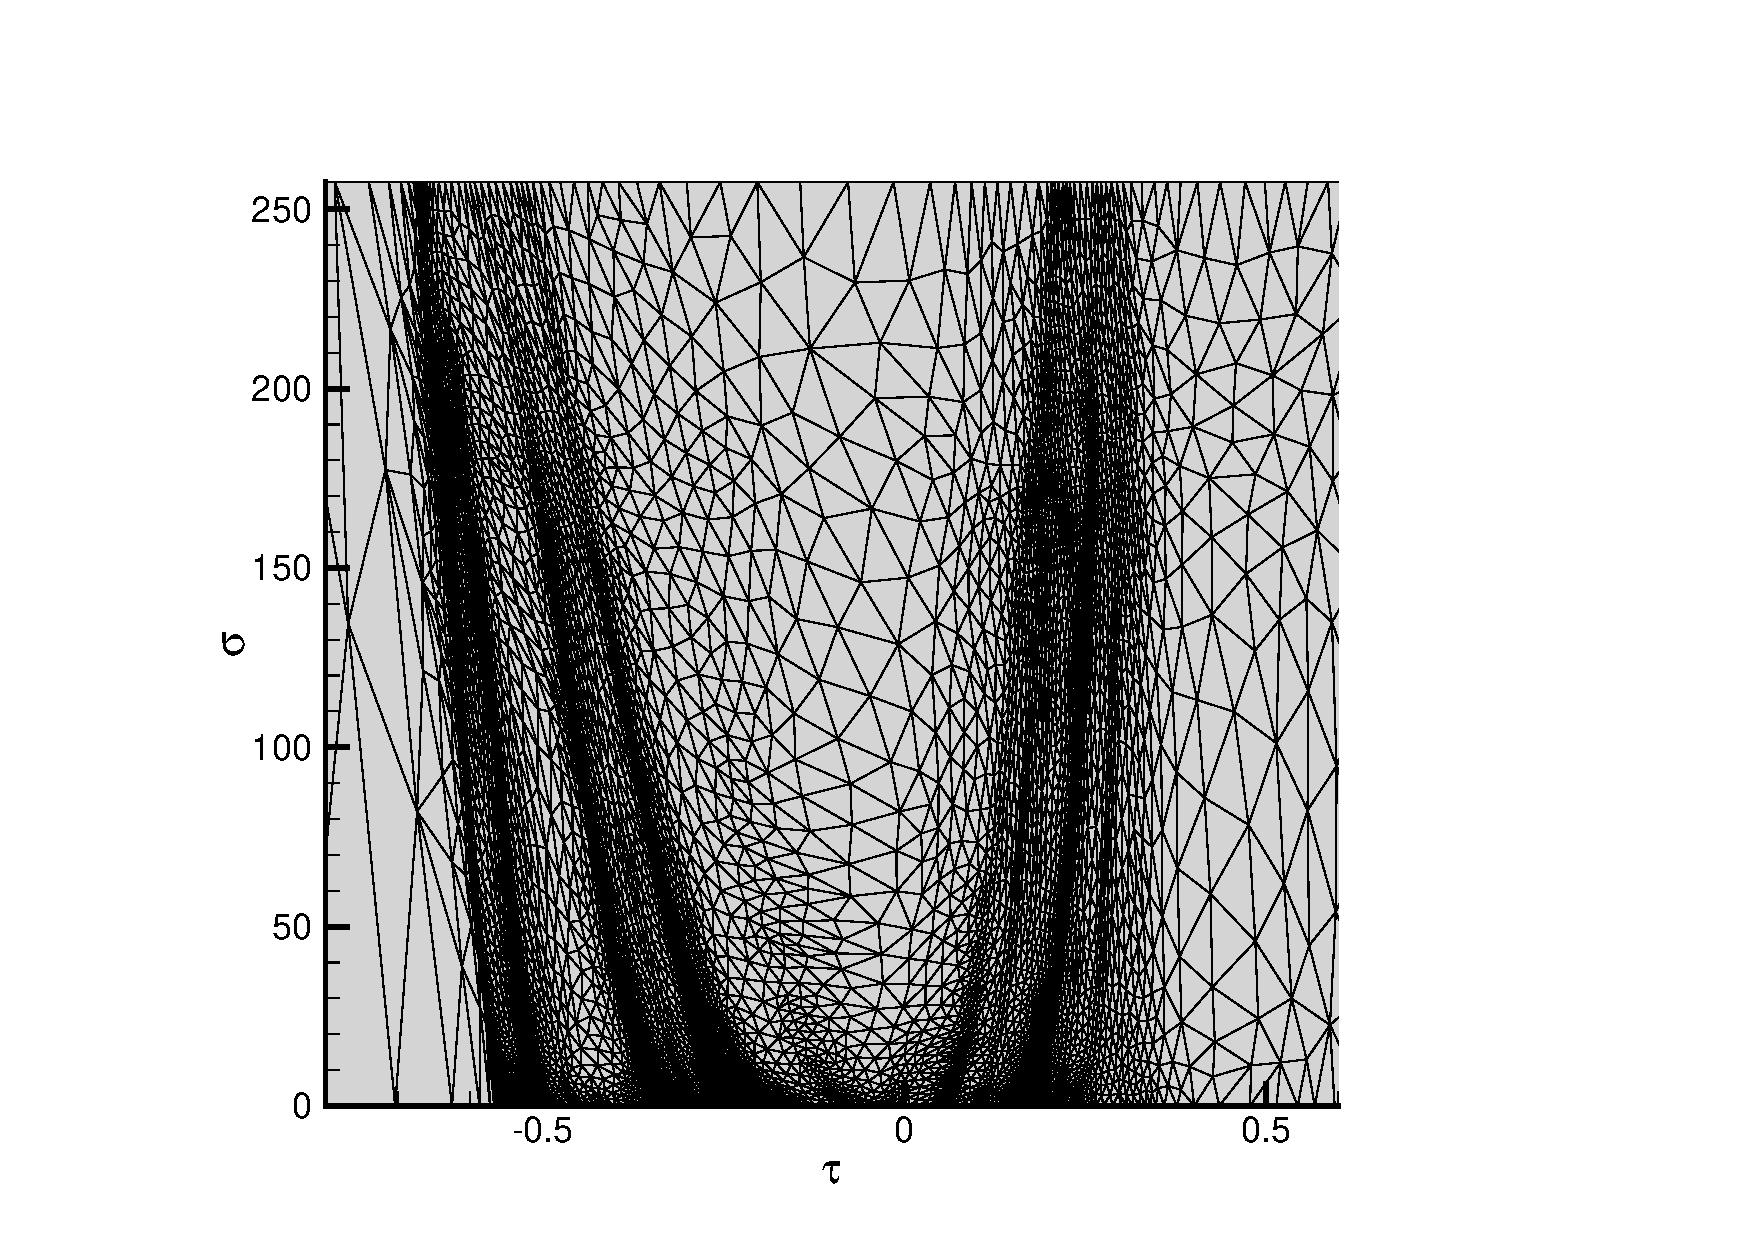
\includegraphics[height=6cm]{../figs/SBW3results/SBW3_P1_8K_mesh_a40_zoomed.pdf}};
\end{tikzpicture}

\begin{tikzpicture}[remember picture,overlay]
  \node[anchor=north east, xshift=1.5cm, yshift=-2cm]
  at (current page.north east) {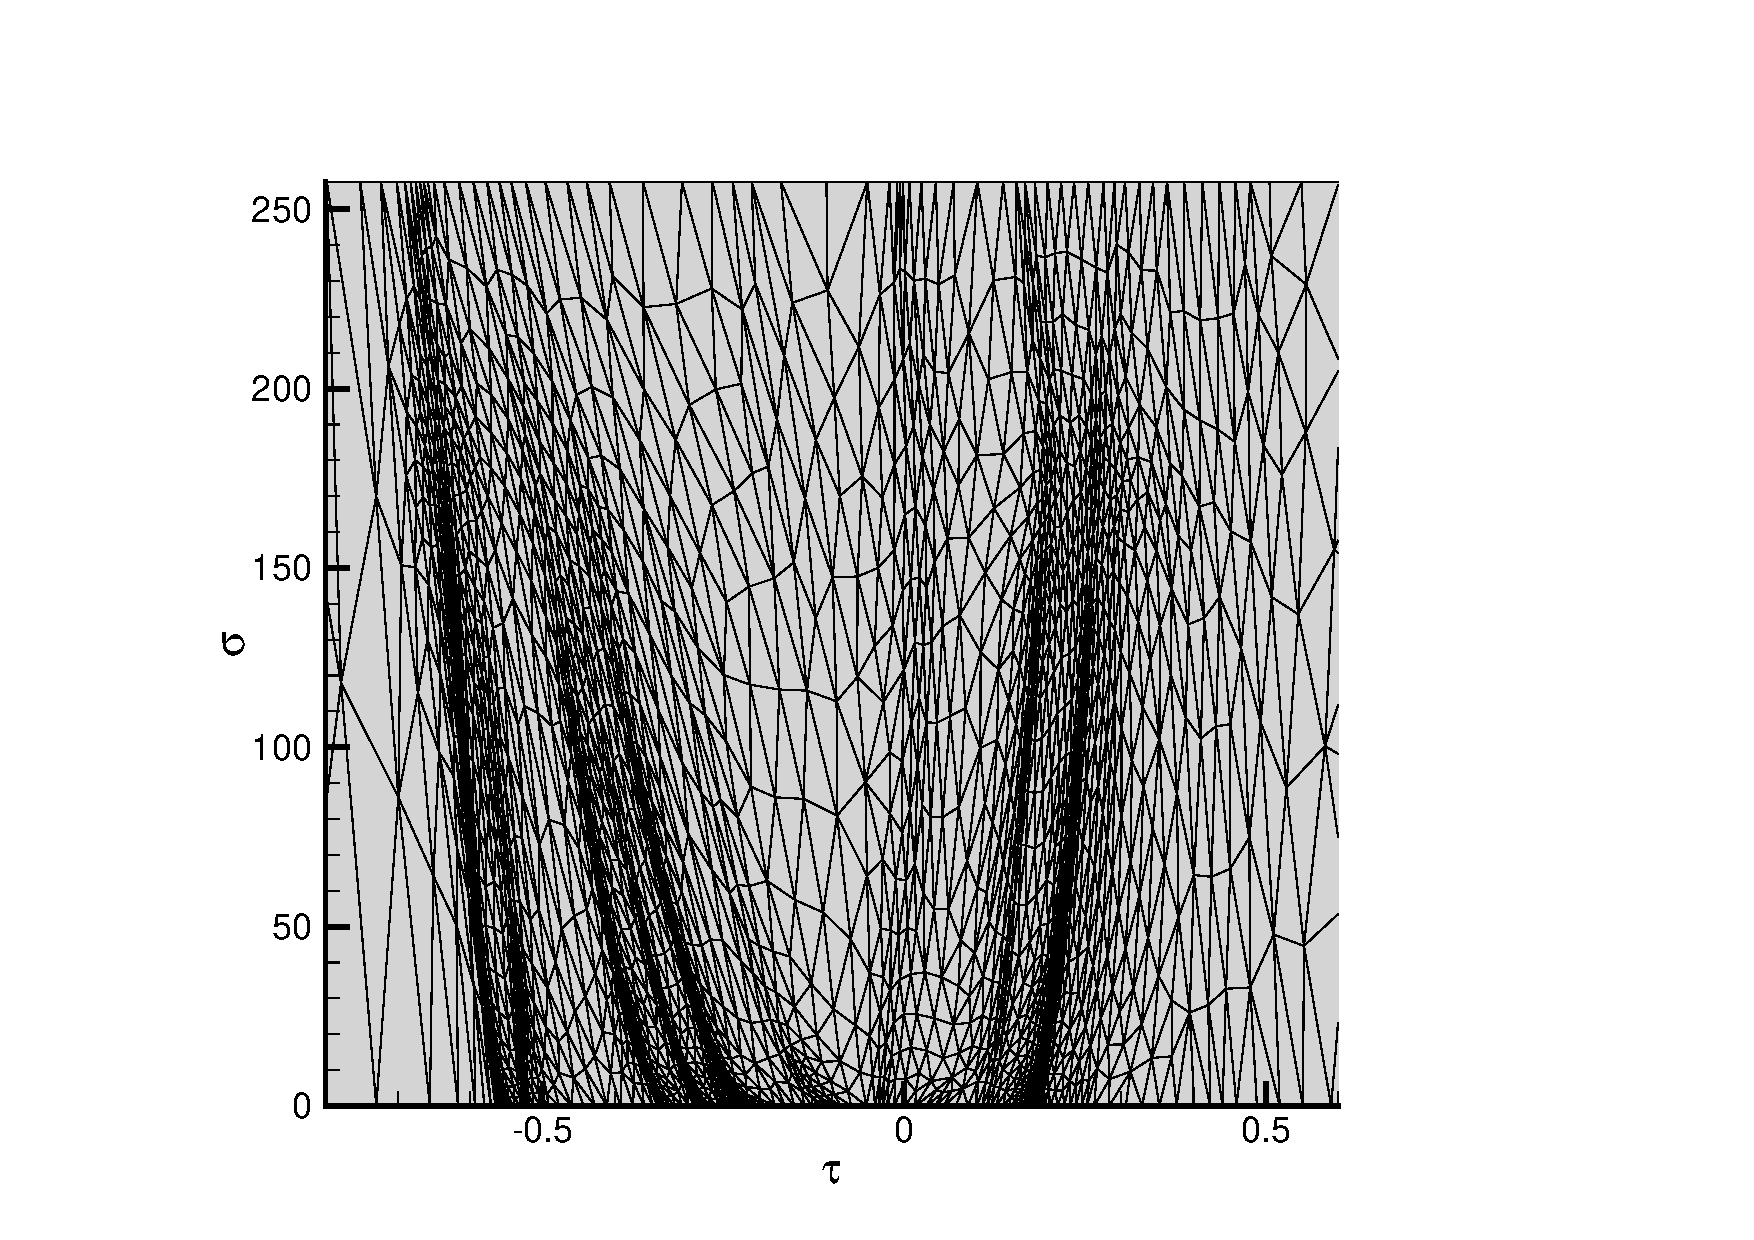
\includegraphics[height=6cm]{../figs/SBW3results/SBW3_P2_8K_mesh_a40_zoomed.pdf}};
\end{tikzpicture}

\end{frame}

%---------------------------------------------------------------%

\stepcounter{sectionframecount}
\begin{frame}[t]{Propagation: Evolution Over Adaptive Cycle, 8K Target DOF}

  \centering
  % Clicking on the thumbnail will launch the external video file.
  \href{run:burgers_mesh_and_primal_combined_8K.mp4}{
\includegraphics[width=0.6\linewidth]{../figs/SBW3results/playVideoSymbol.jpg}}

\end{frame}

%---------------------------------------------------------------%

\stepcounter{sectionframecount}
\begin{frame}[t]{Different Adaptation Outputs and Their Adjoints}

  \begin{tikzpicture}[remember picture,overlay]
    % Place the minipage 1cm from the left and 1cm down from the top
    \node[anchor=north east, xshift=-6.3cm, yshift=-3cm] at (current page.north east) {%
      \begin{minipage}{0.5\textwidth}
      $\mathcal{J}_{\text{BSEL}}$

      \end{minipage}
    };
  \end{tikzpicture}

  \begin{tikzpicture}[remember picture,overlay]
    % Place the minipage 1cm from the left and 1cm down from the top
    \node[anchor=north east, xshift=-6.3cm, yshift=-7cm] at (current page.north east) {%
      \begin{minipage}{0.5\textwidth}
      $\mathcal{J}_p$

      \end{minipage}
    };
  \end{tikzpicture}

  \begin{tikzpicture}[remember picture,overlay]
    \node[anchor=north east, xshift=-6.5cm, yshift=-1.3cm]
    at (current page.north east) {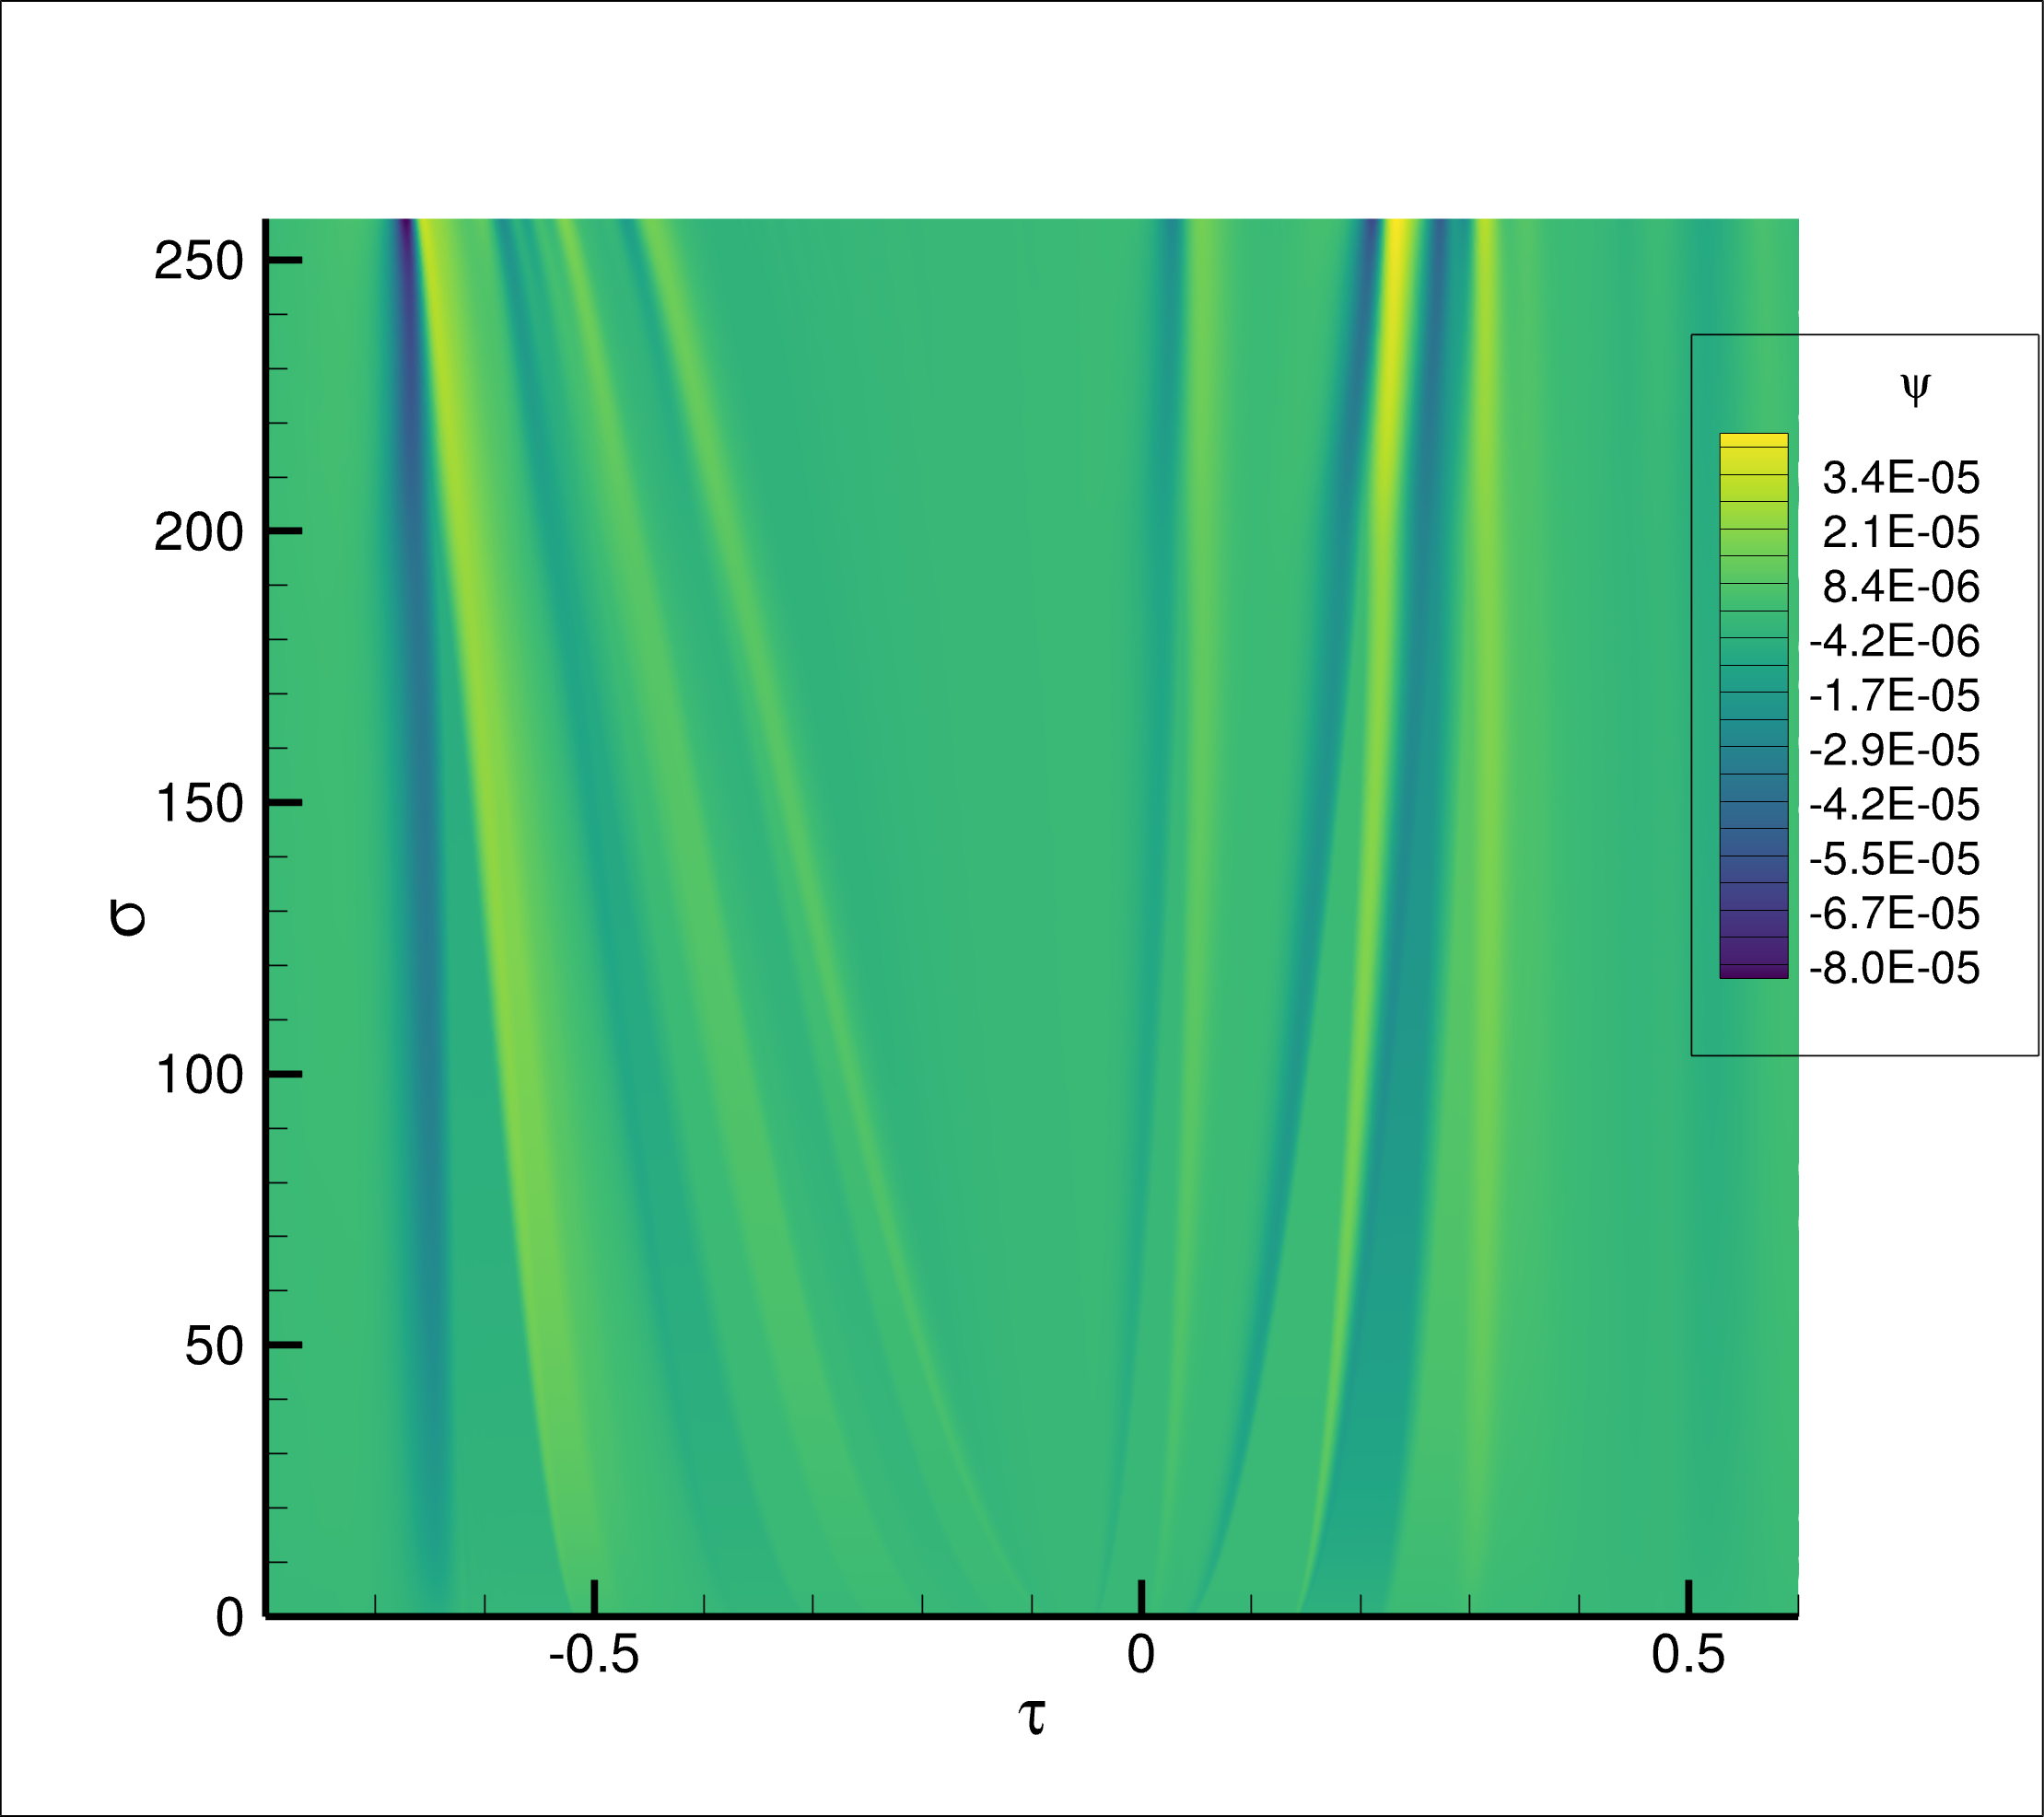
\includegraphics[height=3.9cm]{../figs/SBW3results/adjointAdaptToBSEL_P2_128K.png}};
  \end{tikzpicture}

  \begin{tikzpicture}[remember picture,overlay]
    \node[anchor=north east, xshift=-0.5cm, yshift=-1.3cm]
    at (current page.north east) {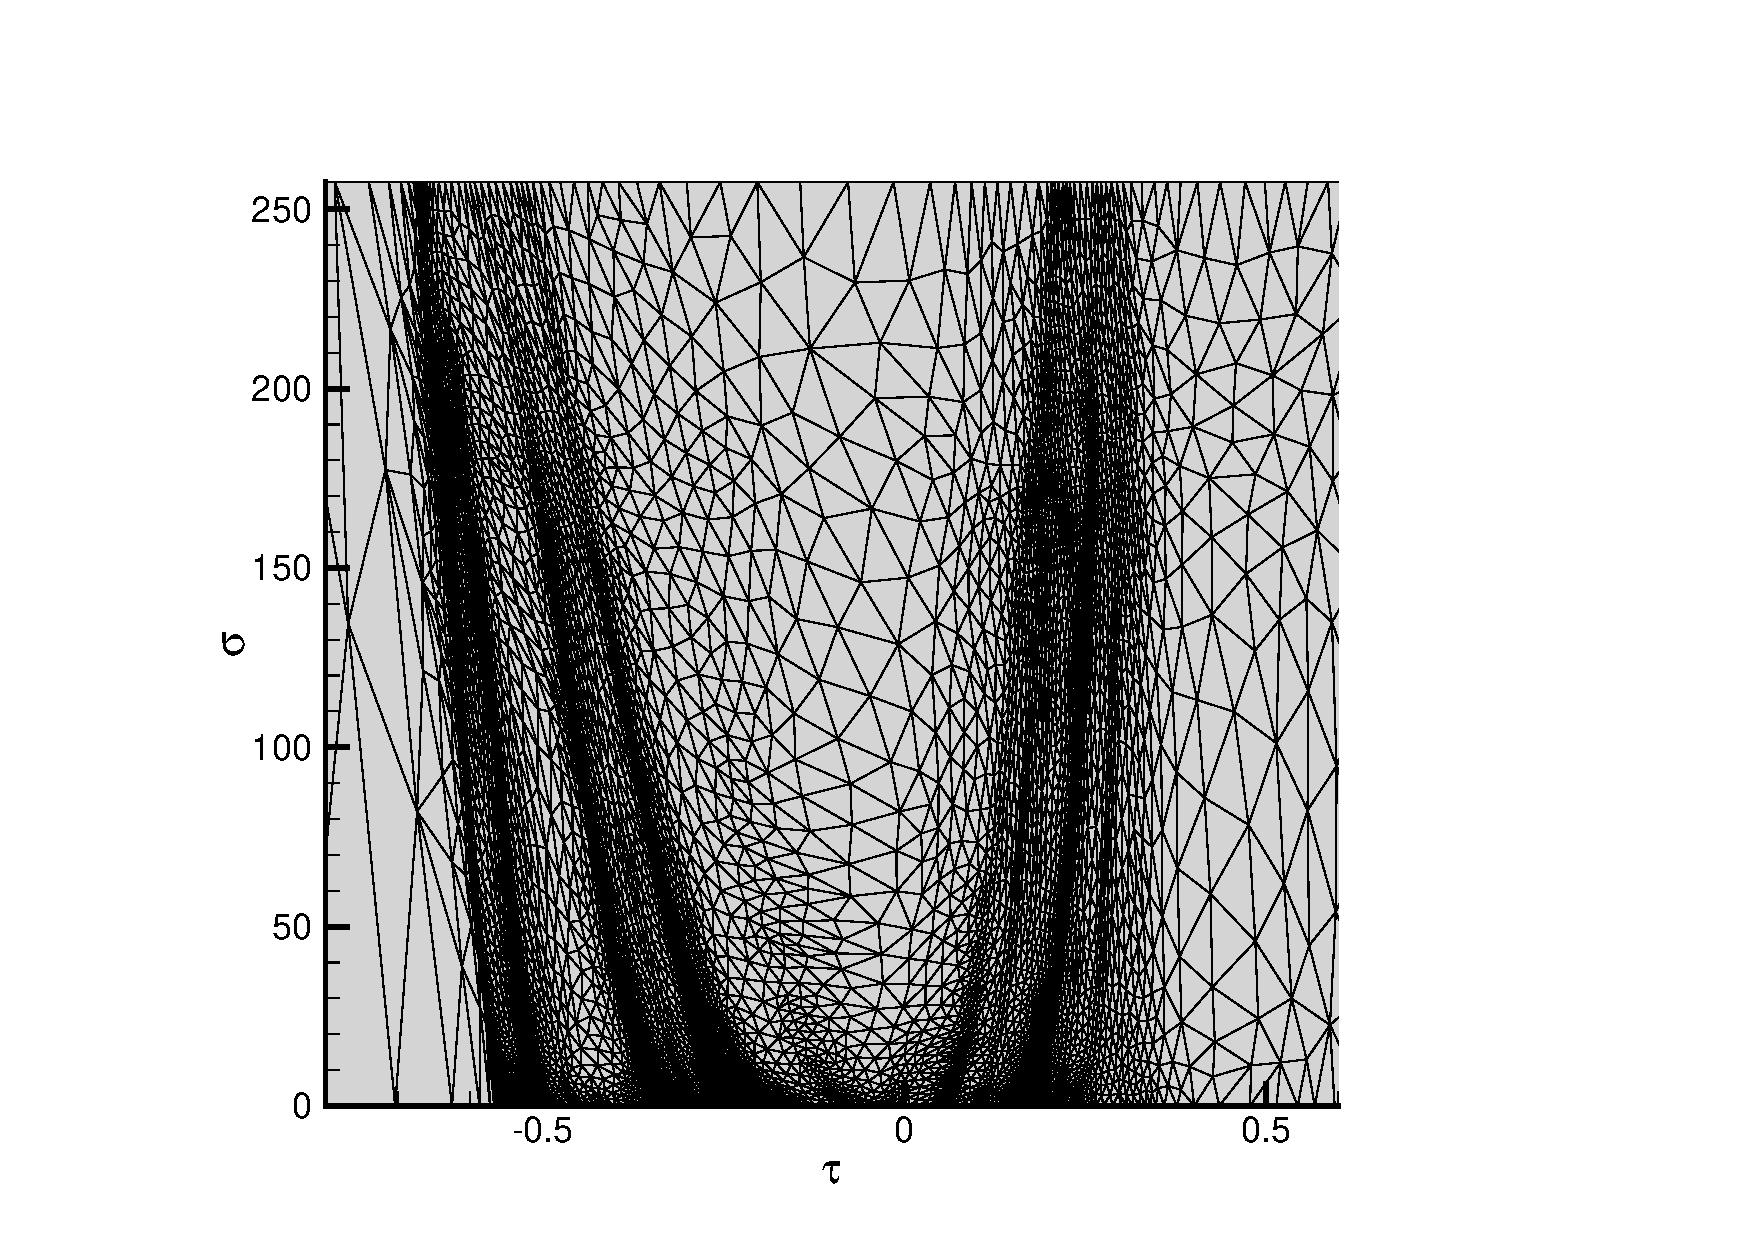
\includegraphics[height=3.9cm]{../figs/SBW3results/SBW3_P1_8K_mesh_a40_zoomed.pdf}};
  \end{tikzpicture}

  \begin{tikzpicture}[remember picture,overlay]
    \node[anchor=north east, xshift=-6.5cm, yshift=-5.3cm]
    at (current page.north east) {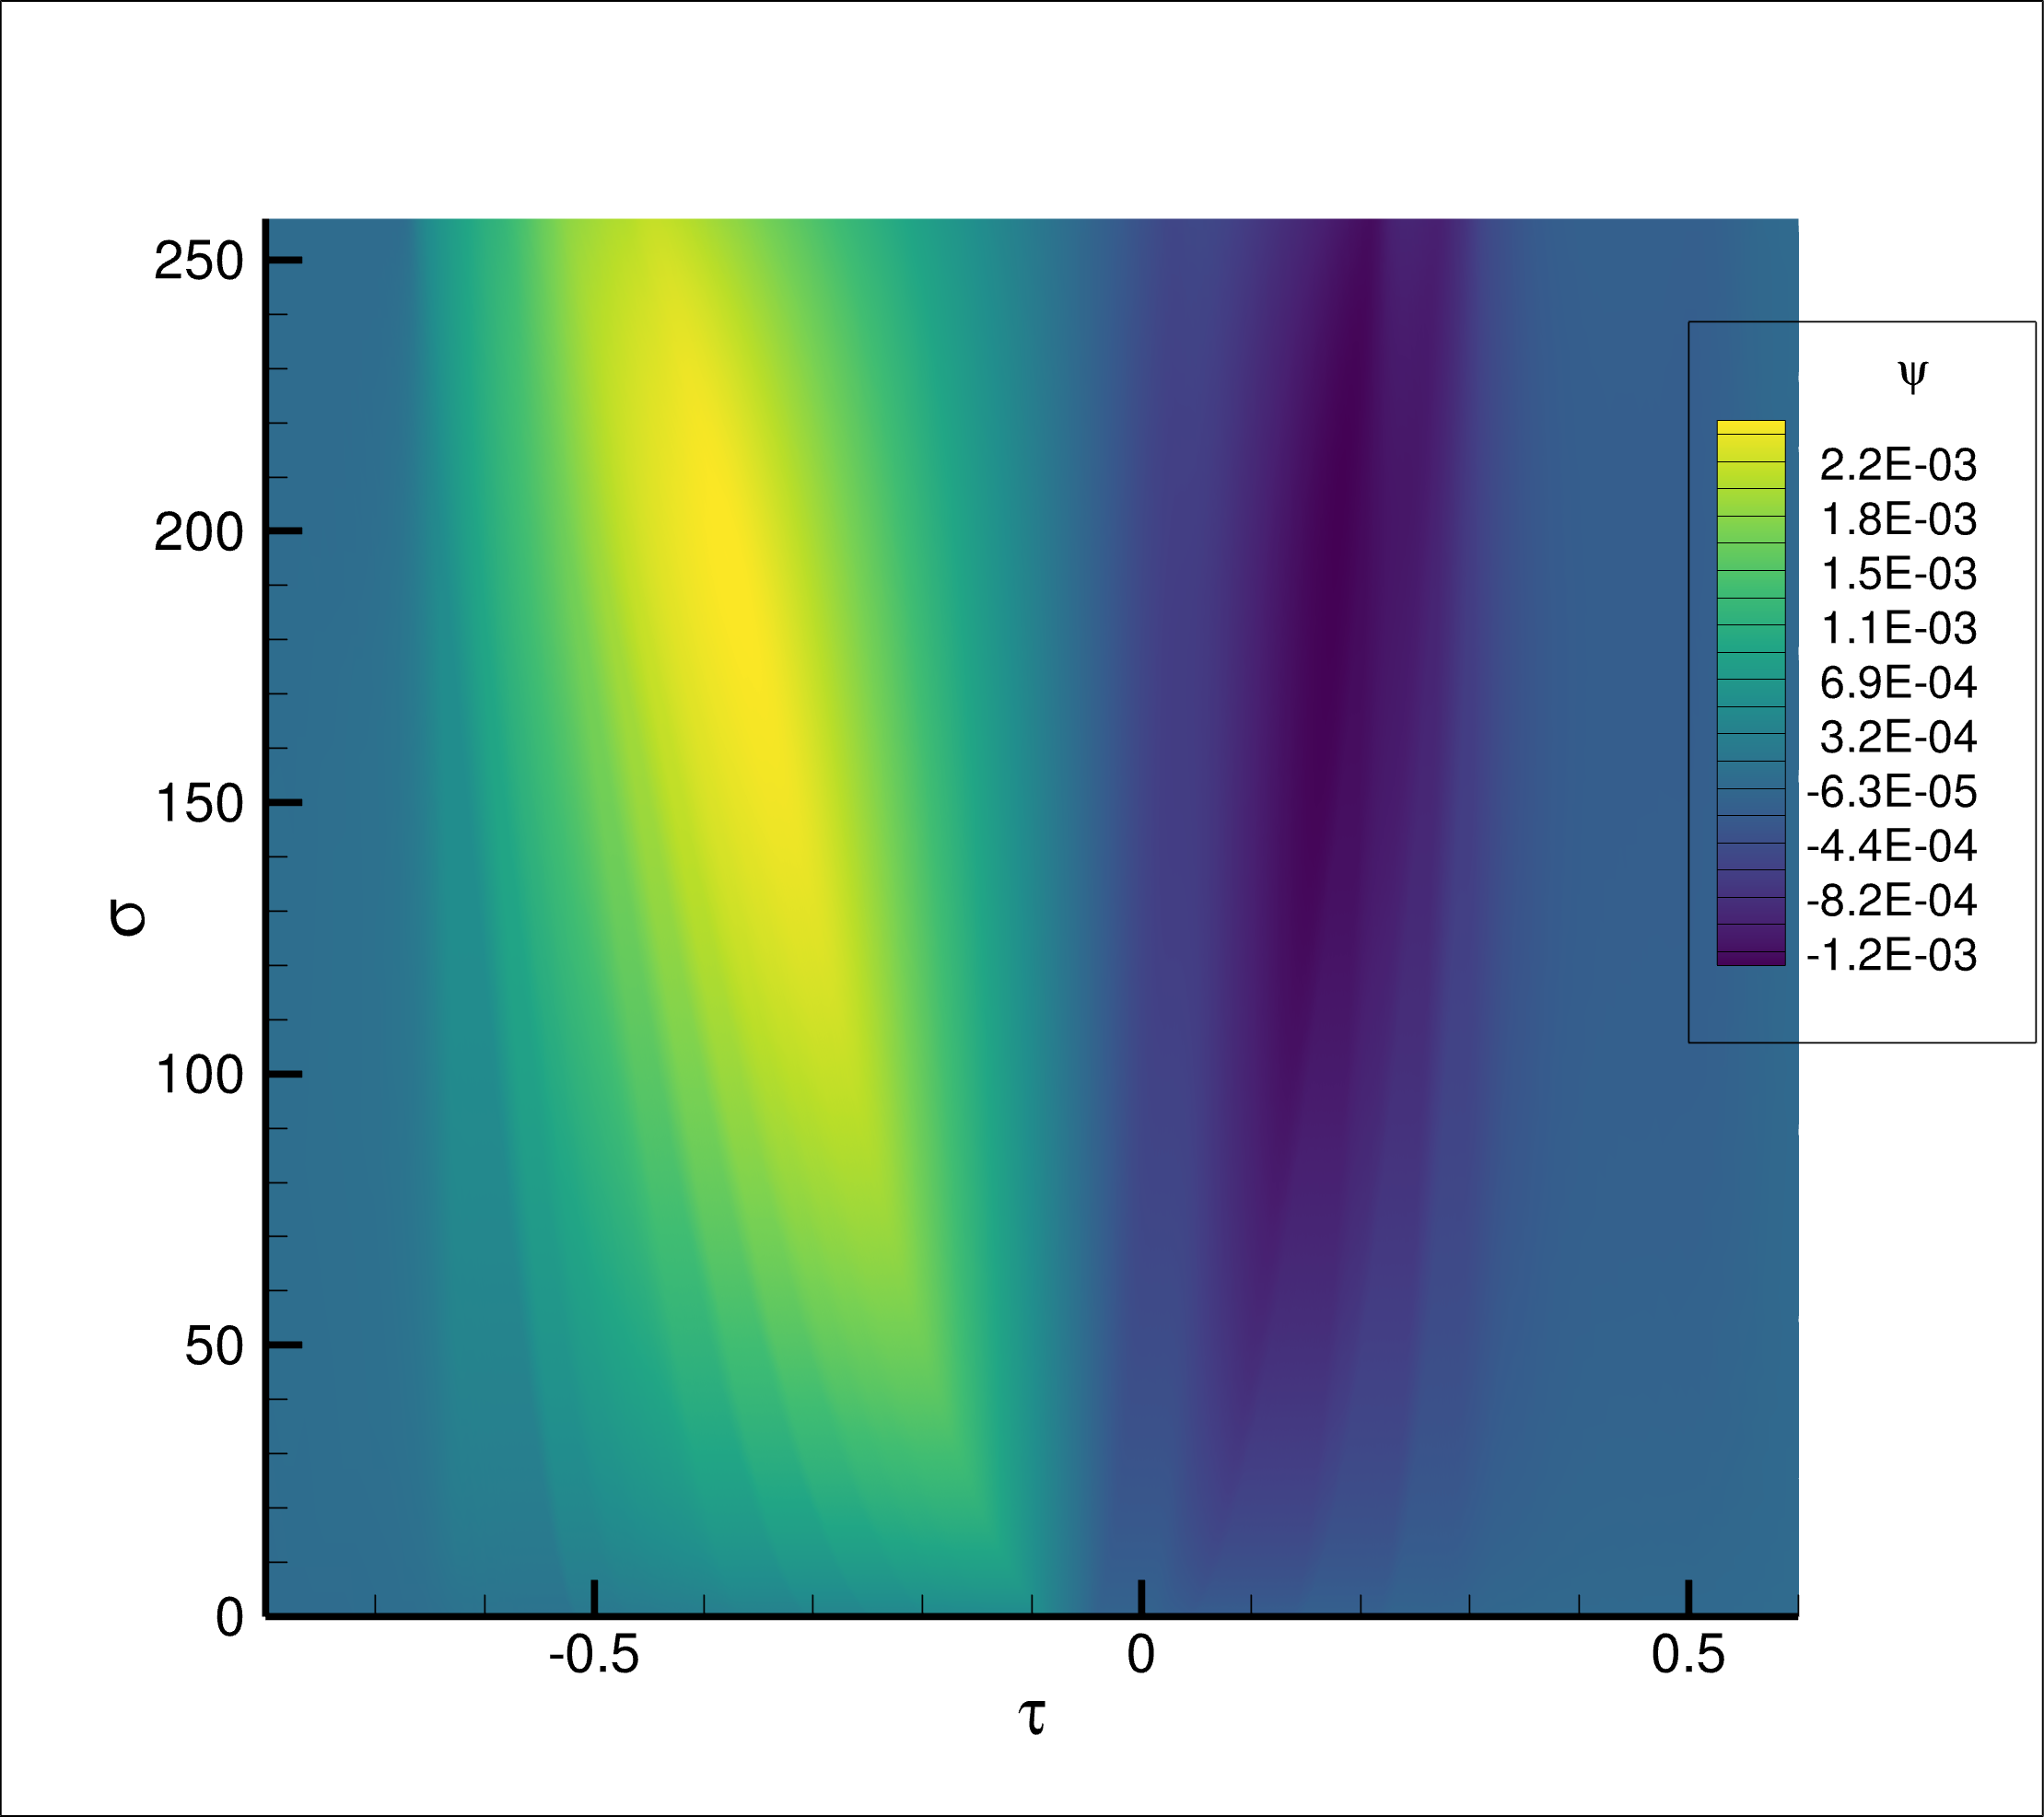
\includegraphics[height=3.9cm]{../figs/SBW3results/adjointAdaptToP2_P2_128K.png}};
  \end{tikzpicture}

  \begin{tikzpicture}[remember picture,overlay]
    \node[anchor=north east, xshift=-0.5cm, yshift=-5.3cm]
    at (current page.north east) {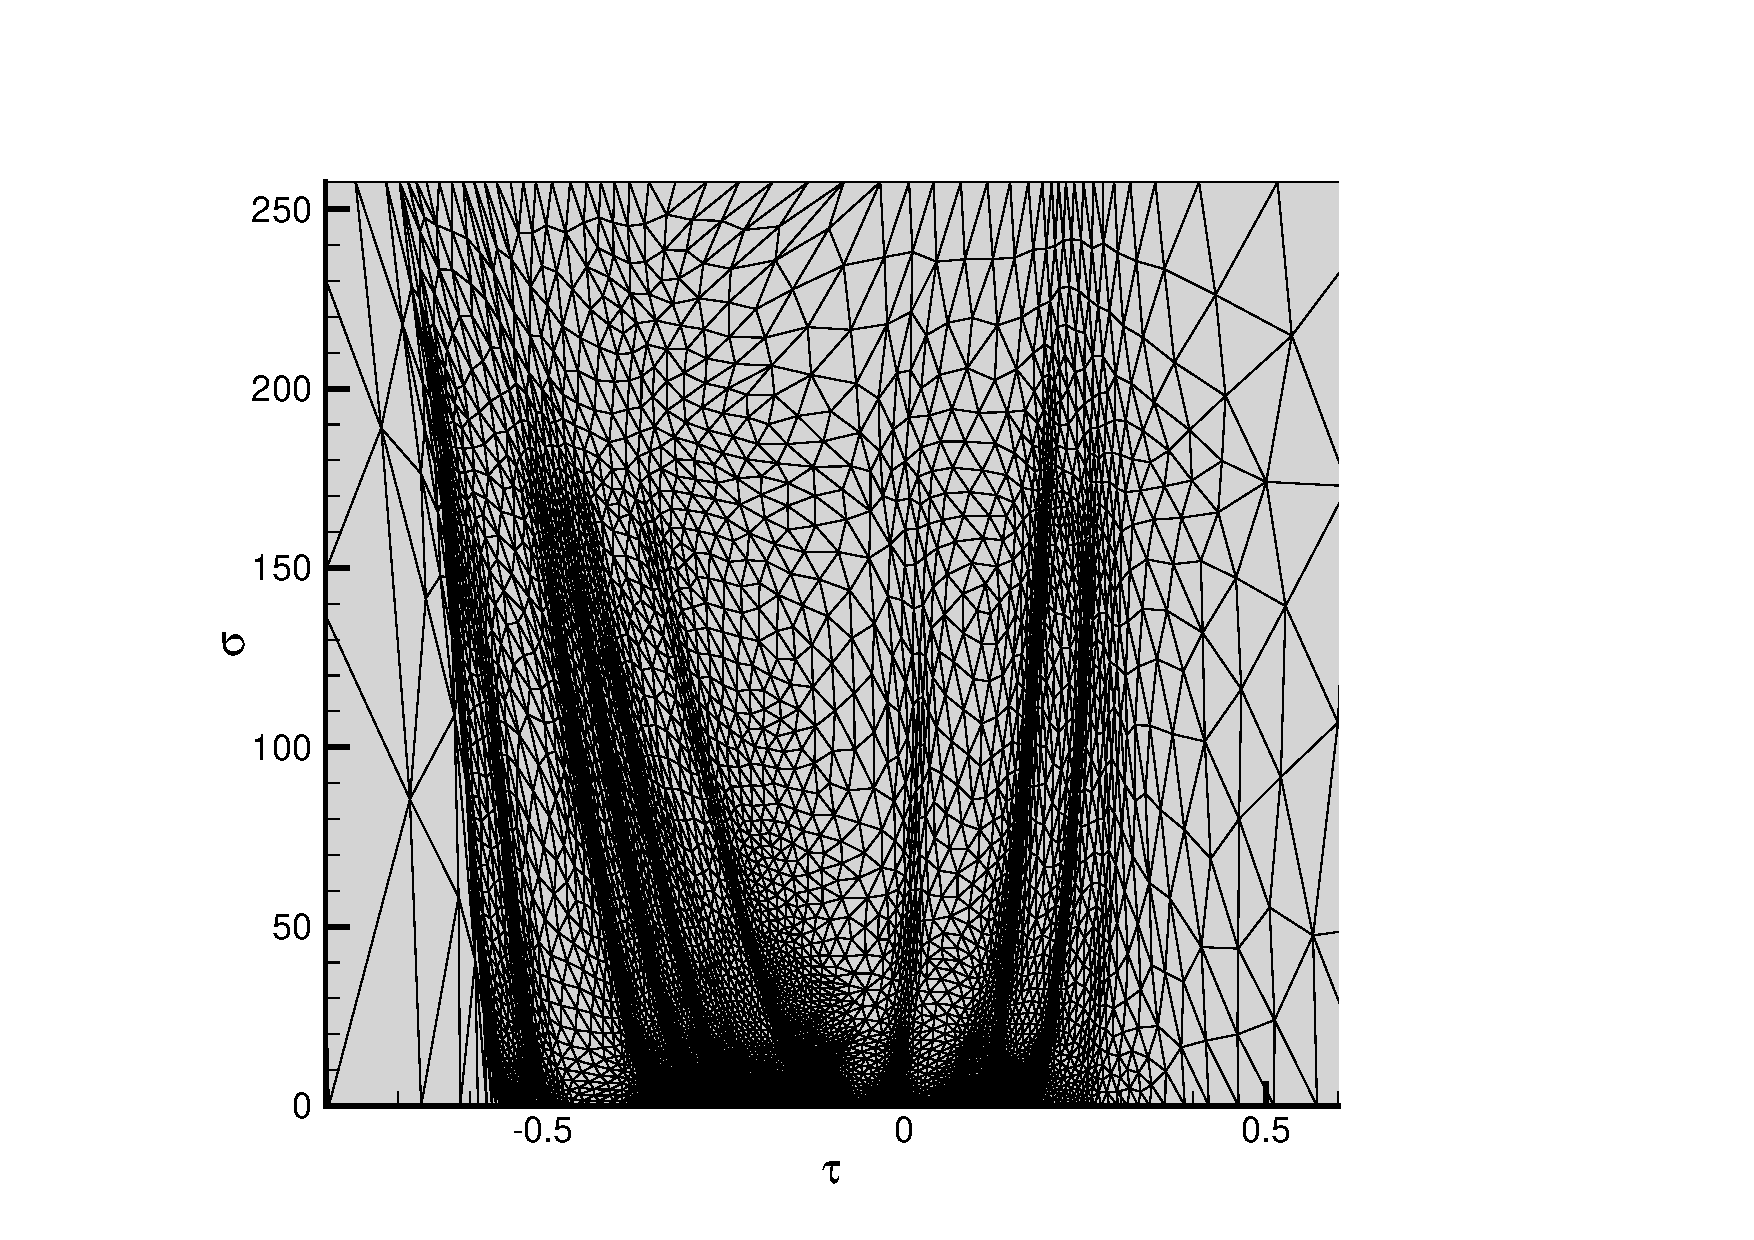
\includegraphics[height=3.9cm]{../figs/SBW3results/SBW3_P1_8K_AdaptToP2_mesh_zoomed.pdf}};
  \end{tikzpicture}

\end{frame}

%---------------------------------------------------------------%

\stepcounter{sectionframecount}
\begin{frame}[t]{At Ground: Pressure Signal and Its Filtering}
\begin{tikzpicture}[remember picture,overlay]
  % Place the minipage 1cm from the left and 1cm down from the top
  \node[anchor=north east, xshift=-4.5cm, yshift=-1.4cm] at (current page.north east) {%
    \begin{minipage}{0.5\textwidth}
    Pressure Signal

    \end{minipage}
  };
\end{tikzpicture}

\begin{tikzpicture}[remember picture,overlay]
  % Place the minipage 1cm from the left and 1cm down from the top
  \node[anchor=north east, xshift=1.5cm, yshift=-1.4cm] at (current page.north east) {%
    \begin{minipage}{0.5\textwidth}
    B-SEL Filter Output

    \end{minipage}
  };
\end{tikzpicture}

\begin{tikzpicture}[remember picture,overlay]
  \node[anchor=north east, xshift=-6.3cm, yshift=-1.8cm]
  at (current page.north east) {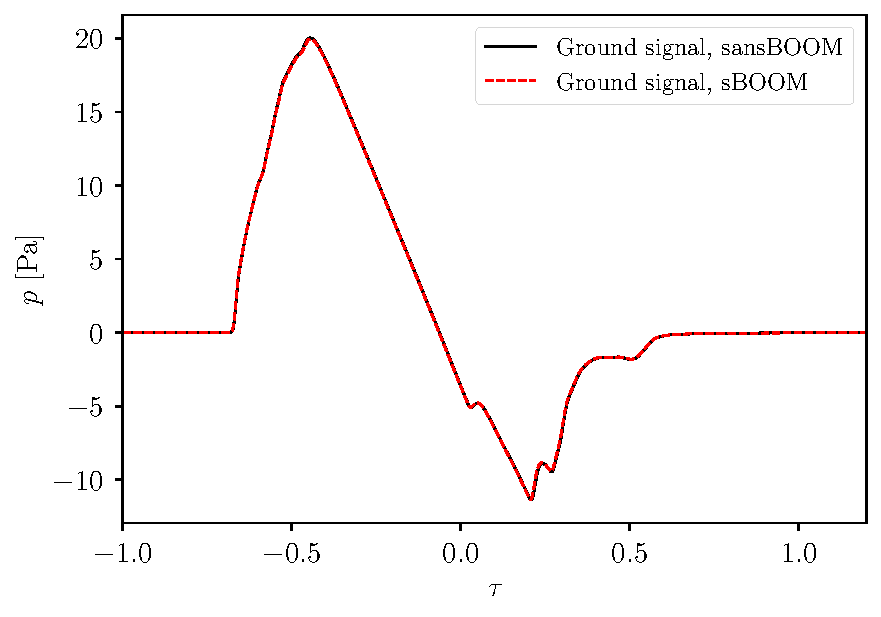
\includegraphics[height=4.3cm]{../figs/SBW3results/ComparisonGround.pdf}};
\end{tikzpicture}

\begin{tikzpicture}[remember picture,overlay]
  \node[anchor=north east, xshift=0.1cm, yshift=-1.8cm]
  at (current page.north east) {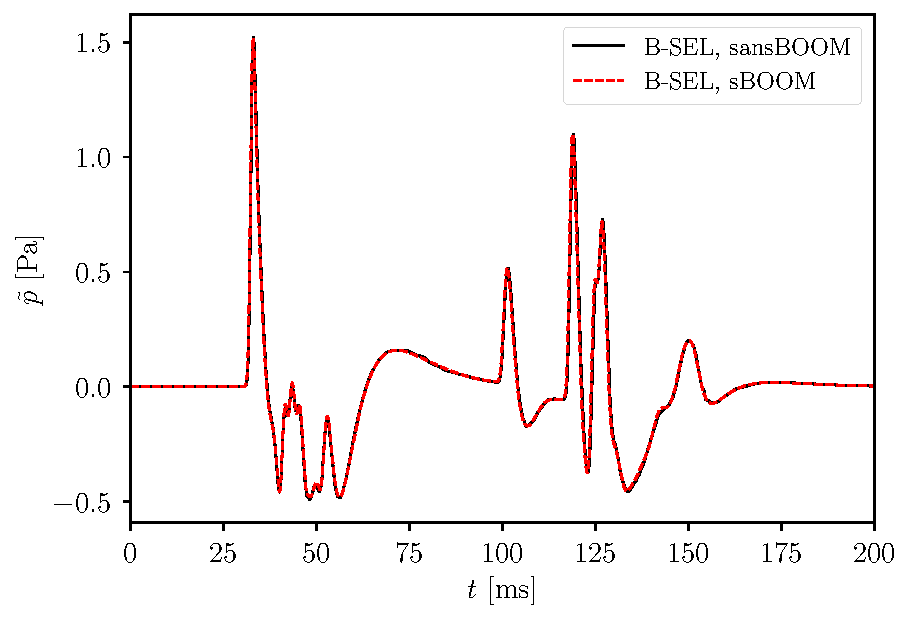
\includegraphics[height=4.3cm]{../figs/SBW3results/comparisonBSEL.pdf}};
\end{tikzpicture}

\vspace{2.6cm}
\scriptsize Comparison with NASA \textit{sBOOM} code\footnotemark:
\begin{itemize}
  \item sansBOOM: 128K DOF in total (space-time).
  \item sBOOM:
  \begin{itemize}
    \item \scriptsize 32K DOF in $\tau$ direction.
    \item 39K steps (marching) in $\sigma$ direction.
    \item 1.2B DOF in total (space-time).
  \end{itemize}
\end{itemize}
\footnotetext{S. K. Rallabhandi et. al. 2023}
\end{frame}

%---------------------------------------------------------------%

\stepcounter{sectionframecount}
\begin{frame}[t]{At Ground: Loudness Convergence with Mesh Refinement}

\begin{tikzpicture}[remember picture,overlay]
  % Place the minipage 1cm from the left and 1cm down from the top
  \node[anchor=north east, xshift=-1.4cm, yshift=-1.8cm] at (current page.north east) {%
    \begin{minipage}{0.5\textwidth}
    B-SEL loudness

    \end{minipage}
  };
\end{tikzpicture}

\begin{tikzpicture}[remember picture,overlay]
  \node[anchor=north east, xshift=-1.8cm, yshift=-2.3cm]
  at (current page.north east) {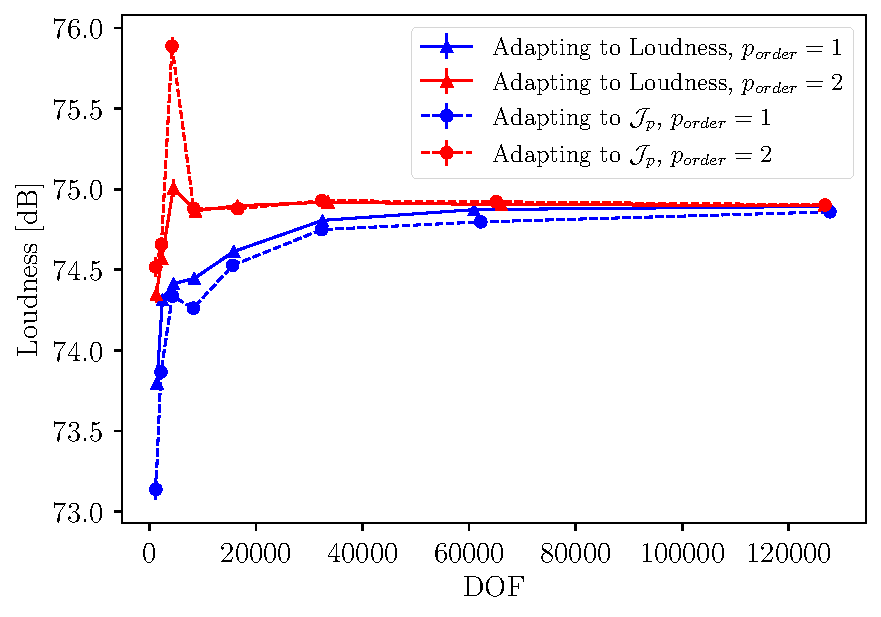
\includegraphics[height=6.5cm]{../figs/SBW3results/SBW3_loudnessGround_adaptToBSEL_comparison.pdf}};
\end{tikzpicture}

\end{frame}

%---------------------------------------------------------------%

\stepcounter{sectionframecount}
\begin{frame}[t]{At Nearfield: Loudness Sensitivity}

\begin{tikzpicture}[remember picture,overlay]
  % Place the minipage 1cm from the left and 1cm down from the top
  \node[anchor=north east, xshift=0cm, yshift=-1.8cm] at (current page.north east) {%
    \begin{minipage}{0.8\textwidth}
    B-SEL loudness sensitivity to nearfield signal

    \end{minipage}
  };
\end{tikzpicture}

\begin{tikzpicture}[remember picture,overlay]
  \node[anchor=north east, xshift=-1.6cm, yshift=-2.3cm]
  at (current page.north east) {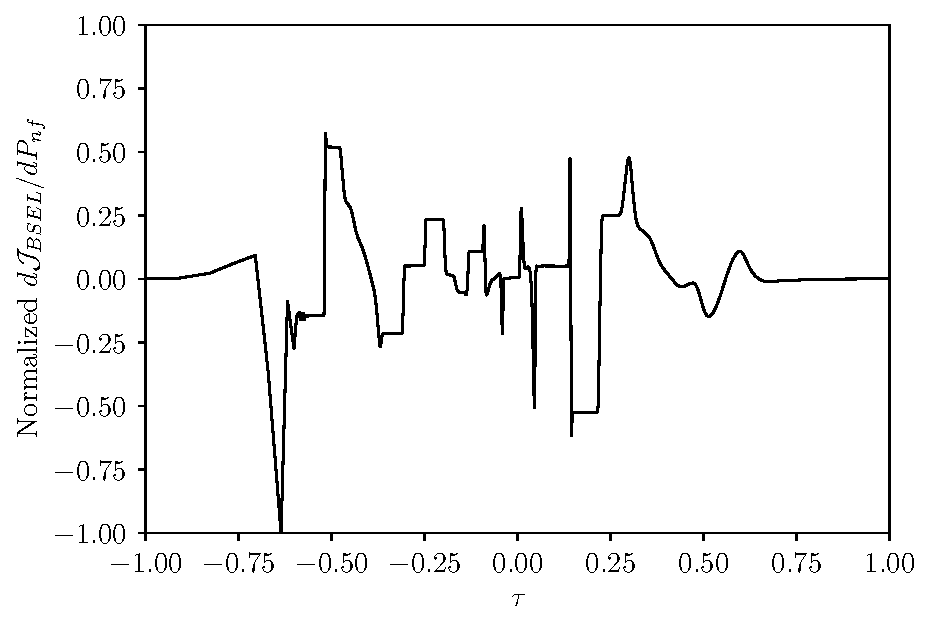
\includegraphics[height=6.5cm]{../figs/SBW3results/loudnessSensistivity.pdf}};
\end{tikzpicture}

\end{frame}

%---------------------------------------------------------------%

%=============================================================================%
%=============================================================================%
%=============================================================================%
% Conclusion


% remove the headline
{
\setbeamertemplate{headline}{} % disable headline for this frame only
\begin{frame}[t]{Concluding Remarks}
    \textbf{Work completed:}
    \begin{itemize}
      \item Higher-order FEM to solve sonic boom propagation problem.
      \item Unstructured space-time mesh adaptation.
      \item Loudness error estimate driving mesh adaptation.
    \end{itemize}

    \textbf{Outcome:}
    \begin{itemize}
      \item Significant reduction in space-time DOF count, at the expense of solving the dual problem.
      \item The above is highlighted when using higher-order solutions, as quadratic solutions converge the output faster than linear solutions.
    \end{itemize}

    \vspace{15pt}
    \textbf{Ongoing effort:}
    \begin{itemize}
      \item Study convergence of loudness sensitivity to nearfield signal.
    \end{itemize}
\end{frame}
}

%=============================================================================%
%=============================================================================%
%=============================================================================%
% Thank you slide

\begin{frame}[plain]
  \vfill
  \centering
  {\usebeamerfont{title}\usebeamercolor[fg]{title}Thanks for the attention! \\ \small Questions?}
  \vfill
\end{frame}

\end{document}

%=============================================================================%
%=============================================================================%
%=============================================================================%
% Original VMSD and Error Estimate separate sections

% %=============================================================================%
% %=============================================================================%
% %=============================================================================%
% % Discretization

% \begin{frame}[plain]
%   \vfill
%   \centering
%   {\usebeamerfont{title}\usebeamercolor[fg]{title}FEM discretization for ADR system}
%   \vfill
% \end{frame}

% \section{FEM discretization for ADR system}

% \setsectionframes{6}

% %---------------------------------------------------------------%

% \stepcounter{sectionframecount}
% \begin{frame}[t]{Analytic problem}
%   \begin{minipage}[t]{1\linewidth}
%     Want to solve general nonlinear ADR system on a 2D domain $\Omega$:

%     \begin{equation}
%       \nabla \cdot \left[\boldsymbol{F}(\boldsymbol{u}) - \boldsymbol{G}(\boldsymbol{u},\nabla \boldsymbol{u}) \right] + \boldsymbol{\mathcal{S}}(\boldsymbol{u},\nabla \boldsymbol{u}) - \boldsymbol{f} = 0 \text{ on } \Omega,
%       \label{e:ADR_pde}
%     \end{equation}

%     \begin{equation}
%       \boldsymbol{u} = \boldsymbol{u}_b \text{ on } \partial \Omega.
%     \end{equation}

%     Where:

%     \begin{itemize}
%       \item $\boldsymbol{u}$: solution of interest (with $m$ states)
%       \item $\boldsymbol{F}$: advective flux operator
%       \item $\boldsymbol{G}$: viscous flux operator
%       \item $\boldsymbol{\mathcal{S}}$: source term operator
%       \item $\boldsymbol{f}$: forcing function
%       \item $\boldsymbol{u}_b$: given boundary function/data
%     \end{itemize}
%   \end{minipage}
% \end{frame}


% %---------------------------------------------------------------%

% \stepcounter{sectionframecount}
% \begin{frame}[t]{Variational Multiscale with Discontinuous Subscales (VMSD) Method}
%   \begin{minipage}[t]{1\linewidth}
%     \vspace{-15pt}
%     \textbf{Discretization of $\Omega$:}

%     \vspace{5pt}
%     $\mathcal{T}_h := \{\kappa\}_{\kappa = 1}^K$ is a triangulation of the domain $\Omega$ into $K$ elements.

%     \vspace{5pt}
%     $\mathcal{E}_h^0$: the set of interior traces.

%     \vspace{5pt}
%     $\mathcal{E}_h^{\partial}$: the set of boundary traces.
%   \end{minipage}

%   \vspace{5pt}
%   \textbf{Propose solution:}

%   $\boldsymbol{u}_h := \bar{\boldsymbol{u}}_{h,p} + \boldsymbol{u}_{h,p^\prime}^\prime$, ~~~~$\bar{\boldsymbol{u}}_{h,p} \in \overline{\mathcal{V}}_{h,p}$, $\boldsymbol{u}^\prime_{h,p^\prime} \in \mathcal{V}^\prime_{h,p^\prime}$

%   \vspace{5pt}
%   \textbf{VMSD solution spaces:}

%   \vspace{-15pt}
%   \begin{equation}
%     \text{(\textit{Coarse} scale) } \overline{\mathcal{V}}_{h,p} := \{\boldsymbol{v}\in [C^0(\Omega)]^m : \boldsymbol{v}|_\kappa \in [\mathcal{P}^p(\kappa)]^m, \forall \kappa \in \mathcal{T}_h\},
%   \end{equation}

%   \vspace{-15pt}
%   \begin{equation}
%     \text{(\textit{Fine} scale) } \mathcal{V}^\prime_{h,p^\prime} := \{\boldsymbol{v}\in [L^2(\Omega)]^m : \boldsymbol{v}|_\kappa \in [\mathcal{P}^{p^\prime}(\kappa)]^m, \forall \kappa \in \mathcal{T}_h\}.
%   \end{equation}

% \end{frame}

% %---------------------------------------------------------------%

% \stepcounter{sectionframecount}
% \begin{frame}[t]{VMSD: residual formulation}
%   \textbf{VMSD weak statement: find $(\bar{\boldsymbol{u}}_{h,p}$, $\boldsymbol{u}^\prime_{h,p^\prime}) \in \overline{\mathcal{V}}_{h,p} \times \mathcal{V}^\prime_{h,p^\prime}$ such that:}
%   \begin{equation}
%     \mathcal{R}_{h}(\bar{\boldsymbol{v}}_{h,p},\boldsymbol{v}^\prime_{h,p^\prime};\bar{\boldsymbol{u}}_{h,p},\boldsymbol{u}^\prime_{h,p^\prime}) = 0,~~\forall (\bar{\boldsymbol{v}}_{h,p},\boldsymbol{v}^\prime_{h,p^\prime}) \in \overline{\mathcal{V}}_{h,p} \times \mathcal{V}^\prime_{h,p^\prime},
%     \label{e:multiscale_weak_statement}
%   \end{equation}

%   where $\mathcal{R}_h$ is the residual form. We break it down as:

%   \begin{equation}
%     \begin{split}
%     \mathcal{R}_h(\bar{\boldsymbol{v}}_{h,p},\boldsymbol{v}^\prime_{h,p^\prime};\bar{\boldsymbol{u}}_{h,p},\boldsymbol{u}^\prime_{h,p^\prime}) :&= \mathcal{R}_F(\bar{\boldsymbol{v}}_{h,p},\boldsymbol{v}^\prime_{h,p^\prime};\bar{\boldsymbol{u}}_{h,p},\boldsymbol{u}^\prime_{h,p^\prime})\\
%     &+\mathcal{R}_G(\bar{\boldsymbol{v}}_{h,p},\boldsymbol{v}^\prime_{h,p^\prime};\bar{\boldsymbol{u}}_{h,p},\boldsymbol{u}^\prime_{h,p^\prime})\\
%     &+\mathcal{R}_S(\bar{\boldsymbol{v}}_{h,p},\boldsymbol{v}^\prime_{h,p^\prime};\bar{\boldsymbol{u}}_{h,p},\boldsymbol{u}^\prime_{h,p^\prime}).
%     \label{e:residual_fluxes_breakdown}
%   \end{split}
%   \end{equation}

%   \textbf{Notation heads-up:}
%   \begin{equation*}
%     (\boldsymbol{a},\boldsymbol{b})_\kappa := \int_\kappa \boldsymbol{a}^T\boldsymbol{b} ~d\kappa,~~~~~~~~~~\left<\boldsymbol{a},\boldsymbol{b}\right>_{\partial \kappa} := \int_{\partial \kappa} \boldsymbol{a}^T\boldsymbol{b}~d\partial\kappa,
%   \end{equation*}
% \end{frame}

% %---------------------------------------------------------------%

% \stepcounter{sectionframecount}
% \begin{frame}[t]{VMSD: advective term and upwinding}

% \textbf{Advective term $\mathcal{R}_F$:}

% \begin{equation}
%   \small
%   \begin{split}
%     {\mathcal{R}}_F&({\bar{\boldsymbol{v}}_{h,p}},\boldsymbol{v}^\prime_{h,p^\prime};\bar{\boldsymbol{u}}_{h,p},\boldsymbol{u}^\prime_{h,p^\prime}) := \\
%     &\sum_{\kappa \in \mathcal{T}_h} \left(-\nabla\bar{\boldsymbol{v}}_{h,p},\boldsymbol{F}(\bar{\boldsymbol{u}}_{h,p} + \boldsymbol{u}^\prime_{h,p^\prime}) \right)_\kappa + \sum_{\epsilon \in \mathcal{E}^\partial_h} \left<\bar{\boldsymbol{v}}_{h,p},\boldsymbol{F}_{n,b}(\bar{\boldsymbol{u}}_{h,p},\boldsymbol{u}_b)\right>_\epsilon\\
%     &+\sum_{\kappa \in \mathcal{T}_h} \Big[ \left(-\nabla\boldsymbol{v}^\prime_{h,p^\prime},\boldsymbol{F}(\bar{\boldsymbol{u}}_{h,p} + \boldsymbol{u}^\prime_{h,p^\prime})\right)_\kappa + \left<\boldsymbol{v}^\prime_{h,p^\prime},\boldsymbol{\mathcal{H}}(\bar{\boldsymbol{u}}_{h,p} + \boldsymbol{u}^\prime_{h,p^\prime},\bar{\boldsymbol{u}}_{h,p},\hat{n}^+) \right>_{\partial\kappa}\Big],
%   \end{split}
% \end{equation}
% where:
% \begin{itemize}
%   \item $\boldsymbol{F}_{n,b}$: Boundary advective flux operator
%   \item $\boldsymbol{\mathcal{H}}$: Upwind flux operator
% \end{itemize}
% \end{frame}

% %---------------------------------------------------------------%

% \stepcounter{sectionframecount}
% \begin{frame}[t]{VMSD: coarse scale viscous term and BR2 stabilization\footnotemark}

% \textbf{Coarse scale viscous term $\mathcal{R}_{G}^{\text{coarse}}$:}

% \vspace{-10pt}
% \begin{equation}
%   \small
%   \begin{split}
%     &\mathcal{R}_G^\text{coarse}(\bar{\boldsymbol{v}}_{h,p};\bar{\boldsymbol{u}}_{h,p},\boldsymbol{u}^\prime_{h,p^\prime}) :=\\
%     &\quad \sum_{\kappa \in \mathcal{T}_h} \Big[ \left(\nabla \bar{\boldsymbol{v}}_{h,p}, \boldsymbol{G}\left(\bar{\boldsymbol{u}}_{h,p} + \boldsymbol{u}^\prime_{h,p^\prime}, \nabla \bar{\boldsymbol{u}}_{h,p} + \nabla \boldsymbol{u}^\prime_{h,p^\prime}\right)\right)_\kappa - \left<\hat{n}\cdot \boldsymbol{G}_{\nabla \boldsymbol{u}}^T \nabla \bar{\boldsymbol{v}}_{h,p},\boldsymbol{u}^\prime_{h,p^\prime}\right>_{\partial \kappa} \Big]\\
%     &- \sum_{\epsilon \in \mathcal{E}_h^\partial} \Big[ \left<\bar{\boldsymbol{v}}_{h,p}, \boldsymbol{G}_{n,b}(\boldsymbol{u}_b,\bar{\boldsymbol{u}}_{h,p},\nabla \bar{\boldsymbol{u}}_{h,p}+\nabla \boldsymbol{u}^\prime_{h,p^\prime}+\eta_\partial\boldsymbol{r}_{p}^\epsilon(\bar{\boldsymbol{u}}_{h,p}-\boldsymbol{u}_b)) \right>_{\epsilon}\\
%     &\qquad\qquad - \left<\hat{n}\cdot \boldsymbol{G}_{\nabla \boldsymbol{u}}^T \nabla \bar{\boldsymbol{v}}_{h,p},\boldsymbol{u}^\prime_{h,p^\prime}\right>_{\epsilon}\Big],
%   \end{split}
% \end{equation}

% \vspace{-20pt}
% where:


% \begin{itemize}
%   \item $\boldsymbol{G}_{\nabla \boldsymbol{u}}^T$: Diffusion tensor
%   \item $\boldsymbol{G}_{n,b}$: Boundary viscous flux operator
%   \item $\boldsymbol{r}_p^\epsilon$: Boundary lifting operator
% \end{itemize}

% \footnotetext{F. Bassi and S. Rebay 2000}
% \end{frame}

% %---------------------------------------------------------------%

% \stepcounter{sectionframecount}
% \begin{frame}[t]{VMSD: source and forcing term}

% \textbf{Source and forcing term $\mathcal{R}_{S}$:}

% \vspace{-10pt}
% \begin{equation}
%   \small
%   \begin{split}
%     \mathcal{R}_S(&{\bar{\boldsymbol{v}}_{h,p}},\boldsymbol{v}^\prime_{h,p^\prime};\bar{\boldsymbol{u}}_{h,p},\boldsymbol{u}^\prime_{h,p^\prime}) := \\
%     &\sum_{\kappa \in \mathcal{T}_h}\left(\bar{\boldsymbol{v}}_{h,p}+\boldsymbol{v}^\prime_{h,p^\prime},\boldsymbol{\mathcal{S}}(\bar{\boldsymbol{u}}_{h,p} + \boldsymbol{u}^\prime_{h,p^\prime},\nabla \bar{\boldsymbol{u}}_{h,p} + \nabla \boldsymbol{u}^\prime_{h,p^\prime}+\boldsymbol{R}_{h,p^\prime}^\kappa(\boldsymbol{u}^\prime_{h,p^\prime})) - \boldsymbol{f}\right)_\kappa,
%   \end{split}
% \end{equation}

% where $\boldsymbol{R}_{h,p}^\kappa$ is an operator representing the sum of the lifting operators on the element $\kappa$:

% \begin{equation}
%   \boldsymbol{R}_{h,p^\prime}^\kappa(\boldsymbol{u}^\prime_{h,p^\prime}) = \sum_{\epsilon \in \partial \kappa} \boldsymbol{r}_{p^\prime}^{\kappa,\epsilon}(\boldsymbol{u}^\prime_{h,p^\prime}).
% \end{equation}

% \end{frame}

% %=============================================================================%
% %=============================================================================%
% %=============================================================================%
% % Output error estimation

% \begin{frame}[plain]
%   \vfill
%   \centering
%   {\usebeamerfont{title}\usebeamercolor[fg]{title}Output Error Estimation}
%   \vfill
% \end{frame}


% \section{Output Error Estimation}

% \setsectionframes{5}

% %---------------------------------------------------------------%

% \stepcounter{sectionframecount}
% \begin{frame}[t]{Output functional}
%   In general, consider output functional of the form:
%   \begin{equation}
%     \mathcal{J}(\boldsymbol{u}) := \int_{\Omega} g_v(\boldsymbol{u})dV + \int_{\partial \Omega} g_b(\boldsymbol{u})dS.
%     \label{e:general_output_functional}
%   \end{equation}

% We define output error as:

% \begin{equation}
%   \varepsilon (\boldsymbol{u}_h) := \mathcal{J}(\boldsymbol{u}) - \mathcal{J}(\boldsymbol{u}_h).
% \end{equation}

% \vspace{8pt}
% For general nonlinear problem, the output error can be approximated using the \textbf{dual weighted residual} (DWR) method.

% \vspace{10pt}
% Needs \textbf{correction} for asymptotically consistent problems.
% \end{frame}

% %---------------------------------------------------------------%

% \stepcounter{sectionframecount}
% \begin{frame}[t]{Residual consistency}
% \vspace{-10pt}
%   \begin{itemize}
%     \item We say the residual form $\mathcal{R}$ is consistent if:
%     \begin{equation}
%       \mathcal{R}(\boldsymbol{v}_h,\boldsymbol{u}) = 0,~~\forall \boldsymbol{v}_h \in \mathcal{V}_h,
%     \end{equation}
%     where $\boldsymbol{u}$ is the exact solution.
%     \item We say the residual form $\mathcal{R}$ is asymptotically consistent if:

%     \begin{equation}
%       \mathcal{R}(\boldsymbol{v}_h,\boldsymbol{u}) = \mathcal{O}(h^\alpha),~~\forall \boldsymbol{v}_h \in \mathcal{V}_h,
%       \label{e:asymptotic_consistent}
%     \end{equation}
%     where $\boldsymbol{u}$ is the exact solution, $\alpha>0$, and $h$ is a characteristic element size in $\mathcal{T}_h$.
%   \end{itemize}

% In our situation:

% \begin{equation}
%   \begin{split}
%   \mathcal{R}(\boldsymbol{v}_h,&\boldsymbol{u}_h) =
%   \mathcal{R}^C(\boldsymbol{v}_h,\boldsymbol{u}_h) + \underbrace{\mathcal{R}^A(\boldsymbol{v}_h,\boldsymbol{u}_h)}_{\text{AV term}}.
%   \end{split}
%   \label{e:residual_C_A_decomposition}
% \end{equation}

% \end{frame}

% %---------------------------------------------------------------%

% \stepcounter{sectionframecount}
% \begin{frame}[t]{Dual problem: mean value linearization}
%   We define the mean value linearizations of the residual and output functional as:

%   \begin{equation}
%      \overline{\mathcal{R}}^\prime [\boldsymbol{u}_h,\boldsymbol{u}](\boldsymbol{v},\boldsymbol{w}) := \int_0^1 \mathcal{R}^\prime[\boldsymbol{u}_h + \theta(\underbrace{\boldsymbol{u}-\boldsymbol{u}_h)}_{\Delta \boldsymbol{u}:=}] (\boldsymbol{v},\boldsymbol{w})~d\theta,
%   \end{equation}

%   \begin{equation}
%       \overline{\mathcal{J}}^\prime [\boldsymbol{u}_h,\boldsymbol{u}](\boldsymbol{w}) := \int_0^1 \mathcal{J}^\prime [\boldsymbol{u}_h + \theta(\boldsymbol{u}-\boldsymbol{u}_h)](\boldsymbol{w})~d\theta.
%   \end{equation}

%   \vspace{10pt}
%   Then, the \textbf{dual} (adjoint) problem is:

%   \vspace{10pt}
%   Find $\boldsymbol{\psi}^\text{mv} \in \mathcal{W} \cup \mathcal{V}_{h}$ such that:

%   \begin{equation}
%       \overline{\mathcal{R}}^\prime[\boldsymbol{u}_h,\boldsymbol{u}](\boldsymbol{\psi}^\text{mv},\boldsymbol{w}) - \overline{\mathcal{J}}^\prime[\boldsymbol{u}_h,\boldsymbol{u}](\boldsymbol{w}) = 0, ~~\forall \boldsymbol{w} \in \mathcal{W} \cup \mathcal{V}_h.
%   \end{equation}

% \end{frame}

% %---------------------------------------------------------------%

% \stepcounter{sectionframecount}
% \begin{frame}[t]{DWR from mean value linearization}
%   We start from:
%   \begin{equation}
%     \begin{split}
%         \varepsilon(\boldsymbol{u}_h) = \mathcal{J}(\boldsymbol{u}) - \mathcal{J}(\boldsymbol{u}_h) &=
%         -\overline{\mathcal{J}}^\prime[\boldsymbol{u}_h,\boldsymbol{u}](\Delta \boldsymbol{u})\\
%         &=-\overline{\mathcal{R}}^\prime[\boldsymbol{u}_h,\boldsymbol{u}_h + \Delta \boldsymbol{u}](\boldsymbol{\psi}^\text{mv},\Delta \boldsymbol{u}).
%     \end{split}
%     \end{equation}
% After some work, we obtain the corrected DWR error expression:

% \begin{equation}
%   \varepsilon(\boldsymbol{u}_h) = -\Big[\mathcal{R}(\boldsymbol{\psi}^\text{mv},\boldsymbol{u}_h) - \mathcal{R}^A(\boldsymbol{\psi}^\text{mv},\boldsymbol{u})\Big].
%   \label{e:dwr_corrected_exact}
% \end{equation}

% \vspace{10pt}
% \textbf{Two issues:}

% \begin{itemize}
%   \item Primal exact solution $\boldsymbol{u}$ is not available.
%   \item The mean value adjoint $\boldsymbol{\psi}^{\text{mv}}$ is not computationally tractable.
% \end{itemize}

% \end{frame}

% %---------------------------------------------------------------%

% \stepcounter{sectionframecount}
% \begin{frame}[t]{Approximations: DWR estimate}
%   \vspace{-10pt}
%   \textbf{First approximation}:

%   \begin{equation}
%     \mathcal{R}^A(\boldsymbol{\psi}^\text{mv},\boldsymbol{u}) \approx
%     \mathcal{R}^A(\boldsymbol{\psi}^\text{mv},\boldsymbol{u}_h),
%   \end{equation}
%   justified on a shock dominated problem with AV.

%   \vspace{5pt}
%   \textbf{Second approximation:} Tractable adjoint

%   \vspace{10pt}
%   $\boldsymbol{\psi}^\text{mv}$ is approximated with a numerical adjoint $\boldsymbol{\psi}_{\hat{h}}$ defined by\footnotemark:

%   Find $\boldsymbol{\psi}_{\hat{h}} \in \mathcal{V}_{\hat{h}}$ such that:

% \begin{equation}
%   \mathcal{J}^\prime[\boldsymbol{u}_h](\tilde{\boldsymbol{u}}) - \mathcal{R}^\prime[\boldsymbol{u}_h](\boldsymbol{\psi}_{\hat{h}},\tilde{\boldsymbol{u}}) = \mathcal{J}^*(\boldsymbol{\psi}_{\hat{h}}) - \mathcal{R}^*(\tilde{\boldsymbol{u}},\boldsymbol{\psi}_{\hat{h}}),~~\forall \tilde{\boldsymbol{u}} \in \mathcal{V}_{\hat{h}}.
% \end{equation}

% \vspace{10pt}
% \textbf{DWR error estimate:}
% \begin{equation}
%   \mathcal{J}(\boldsymbol{u}) - \mathcal{J}(\boldsymbol{u}_h) \approx -\Big[\mathcal{R}(\boldsymbol{\psi}_{\hat{h}},\boldsymbol{u}_h) - \mathcal{R}^A(\boldsymbol{\psi}_{\hat{h}},\boldsymbol{u}_h)\Big].
% \end{equation}

% \footnotetext{M. Yano and D. L. Darmofal 2012}

% \end{frame}